%%%%%%%%%%%%%%%%%%%%%%%%%%%%%%%%%%%%%%%%
% Masters/Doctoral Thesis 
% LaTeX Template
% Version 2.5 (27/8/17)
%
% This template was downloaded from:
% http://www.LaTeXTemplates.com
%
% Version 2.x major modifications by:
% Vel (vel@latextemplates.com)
%
% This template is based on a template by:
% Steve Gunn (http://users.ecs.soton.ac.uk/srg/softwaretools/document/templates/)
% Sunil Patel (http://www.sunilpatel.co.uk/thesis-template/)
%
% Template license:
% CC BY-NC-SA 3.0 (http://creativecommons.org/licenses/by-nc-sa/3.0/)
%
%%%%%%%%%%%%%%%%%%%%%%%%%%%%%%%%%%%%%%%%%

%----------------------------------------------------------------------------------------
%	PACKAGES AND OTHER DOCUMENT CONFIGURATIONS
%----------------------------------------------------------------------------------------

\documentclass[
12pt, % The default document font size, options: 10pt, 11pt, 12pt
 % Two side (alternating margins) for binding by default, uncomment to switch to one side
english, % ngerman for German
doublespacing, % Single line spacing, alternatives: onehalfspacing or doublespacing
%draft, % Uncomment to enable draft mode (no pictures, no links, overfull hboxes indicated)
%nolistspacing, % If the document is onehalfspacing or doublespacing, uncomment this to set spacing in lists to single
nolistspacing,
%liststotoc, % Uncomment to add the list of figures/tables/etc to the table of contents
%toctotoc, % Uncomment to add the main table of contents to the table of contents
%parskip, % Uncomment to add space between paragraphs
%nohyperref, % Uncomment to not load the hyperref package
headsepline, % Uncomment to get a line under the header
%chapterinoneline, % Uncomment to place the chapter title next to the number on one line
%consistentlayout, % Uncomment to change the layout of the declaration, abstract and acknowledgements pages to match the default layout
]{MastersDoctoralThesis} % The class file specifying the document structure

\usepackage[utf8]{inputenc} % Required for inputting international characters
\usepackage[T1]{fontenc} % Output font encoding for international characters

\usepackage{mathpazo} % Use the Palatino font by default

\usepackage[backend=bibtex,style=ieee,maxbibnames=3]{biblatex} % Use the bibtex backend with the authoryear citation style (which resembles APA)

\addbibresource{ref.bib} % The filename of the bibliography

\usepackage[autostyle=true]{csquotes} % Required to generate language-dependent quotes in the bibliography

\usepackage{multirow} % Required for some table settings

\usepackage{float} % using % to fix position of figures and tables 

\usepackage{etoolbox}


%----------------------------------------------------------------------------------------
%	MARGIN SETTINGS
%----------------------------------------------------------------------------------------

\geometry{
	paper=a4paper, % Change to letterpaper for US letter
	inner=3cm, % Inner margin
	outer=3cm, % Outer margin
	bindingoffset=.5cm, % Binding offset
	top=2cm, % Top margin
	bottom=2cm, % Bottom margin
	%showframe, % Uncomment to show how the type block is set on the page
}

%----------------------------------------------------------------------------------------
%	THESIS INFORMATION
%----------------------------------------------------------------------------------------

\thesistitle{Developments to established dose-finding methodologies for application in trials with complex and innovative designs} % Your thesis title, this is used in the title and abstract, print it elsewhere with \ttitle
\supervisor{Prof. Lucinda \textsc{Billingham}}
% Your supervisor's name, this is used in the title page, print it elsewhere with \supname
\supervisorTWO{Dr. Kristian \textsc{Brock}}
\examiner{} % Your examiner's name, this is not currently used anywhere in the template, print it elsewhere with \examname
\degree{Doctor of Philosophy} % Your degree name, this is used in the title page and abstract, print it elsewhere with \degreename
\author{Amit \textsc{Patel}} % Your name, this is used in the title page and abstract, print it elsewhere with \authorname
\addresses{} % Your address, this is not currently used anywhere in the template, print it elsewhere with \addressname

\subject{Biological Sciences} % Your subject area, this is not currently used anywhere in the template, print it elsewhere with \subjectname
\keywords{} % Keywords for your thesis, this is not currently used anywhere in the template, print it elsewhere with \keywordnames
\university{\href{https://www.birmingham.ac.uk/index.aspx}{University of Birmingham}} % Your university's name and URL, this is used in the title page and abstract, print it elsewhere with \univname
\department{\href{https://www.birmingham.ac.uk/university/colleges/mds/index.aspx}{College of Medical and Dental Sciences}} % Your department's name and URL, this is used in the title page and abstract, print it elsewhere with \deptname
\group{\href{https://www.birmingham.ac.uk/research/cancer-genomics/index.aspx}{Institute of Cancer and Genomic Sciences}} % Your research group's name and URL, this is used in the title page, print it elsewhere with \groupname
\faculty{\href{http://faculty.university.com}{Faculty Name}} % Your faculty's name and URL, this is used in the title page and abstract, print it elsewhere with \facname

\AtBeginDocument{
\hypersetup{pdftitle=\ttitle} % Set the PDF's title to your title
\hypersetup{pdfauthor=\authorname} % Set the PDF's author to your name
\hypersetup{pdfkeywords=\keywordnames} % Set the PDF's keywords to your keywords
}

\begin{document}

\frontmatter % Use roman page numbering style (i, ii, iii, iv...) for the pre-content pages

\pagestyle{plain} % Default to the plain heading style until the thesis style is called for the body content

%----------------------------------------------------------------------------------------
%	TITLE PAGE
%----------------------------------------------------------------------------------------

\begin{titlepage}
\begin{center}

%\vspace*{.06\textheight}
%{\scshape\LARGE \univname\par}\vspace{0.5cm} % University name
\textsc{\Large Doctoral Thesis}\\[0.5cm] % Thesis type

\HRule \\[0.2cm] % Horizontal line
{\Large \bfseries \ttitle\par}\vspace{0.2cm} % Thesis title
\HRule \\[0.5cm] % Horizontal line
 
\begin{minipage}[t]{0.3\textwidth}
\begin{flushleft} \large
\emph{Author:}\\
\href{https://uk.linkedin.com/in/amit-patel-0b718111b}{\authorname} % Author name - remove the \href bracket to remove the link
\end{flushleft}
\end{minipage}
\begin{minipage}[t]{0.5\textwidth}
\begin{flushright} \large
\emph{Supervisor:} \\
\href{https://www.birmingham.ac.uk/staff/profiles/cancer-genomic/billingham-lucinda.aspx}{\supname}\\ % Supervisor name - remove the \href bracket to remove the link  
\href{https://www.kristianbrock.com/}{\supnameTWO}
\end{flushright}
\end{minipage}\\[2.5cm]
 


\large \textit{A thesis submitted in fulfillment of the requirements\\ for the degree of \degreename}\\[2.5cm] % University requirement text



\begin{flushright}
\groupname\\\deptname\\\univname\\\today
\end{flushright}

%\includegraphics{Logo} % University/department logo - uncomment to place it
 
\vfill
\end{center}
\end{titlepage}

%----------------------------------------------------------------------------------------
%	DECLARATION PAGE
%----------------------------------------------------------------------------------------

%\begin{declaration}
%\addchaptertocentry{\authorshipname} % Add the declaration to the table of contents
%\noindent I, \authorname, declare that this thesis titled, \enquote{\ttitle} and the work presented in it are my own. I confirm that:

%\begin{itemize} 
%\item This work was done wholly or mainly while in candidature for a research degree at this University.
%\item Where any part of this thesis has previously been submitted for a degree or any other qualification at this University or any other institution, this has been clearly stated.
%\item Where I have consulted the published work of others, this is always clearly attributed.
%\item Where I have quoted from the work of others, the source is always given. With the exception of such quotations, this thesis is entirely my own work.
%\item I have acknowledged all main sources of help.
%\item Where the thesis is based on work done by myself jointly with others, I have made clear exactly what was done by others and what I have contributed myself.\\
%\end{itemize}
 
%\noindent Signed:\\
%\rule[0.5em]{25em}{0.5pt} % This prints a line for the signature
 
%\noindent Date:\\
%\rule[0.5em]{25em}{0.5pt} % This prints a line to write the date
%\end{declaration}

%\cleardoublepage

%----------------------------------------------------------------------------------------
%	QUOTATION PAGE
%----------------------------------------------------------------------------------------

%\vspace*{0.2\textheight}

%\noindent\enquote{\itshape This is where the fun begins.}\bigbreak

%\hfill Anakin Skywalker

%----------------------------------------------------------------------------------------
%	ABSTRACT PAGE
%----------------------------------------------------------------------------------------

\begin{abstract}
\addchaptertocentry{\abstractname} % Add the abstract to the table of contents
Insert abstract here\ldots
\end{abstract}

%----------------------------------------------------------------------------------------
%	ACKNOWLEDGEMENTS
%----------------------------------------------------------------------------------------

\begin{acknowledgements}
\addchaptertocentry{\acknowledgementname} % Add the acknowledgements to the table of contents
Acknowledge people here \ldots
\end{acknowledgements}

%----------------------------------------------------------------------------------------
%	LIST OF CONTENTS/FIGURES/TABLES PAGES
%----------------------------------------------------------------------------------------

\tableofcontents % Prints the main table of contents

\listoffigures % Prints the list of figures

\listoftables % Prints the list of tables

%----------------------------------------------------------------------------------------
%	ABBREVIATIONS
%----------------------------------------------------------------------------------------

%\begin{abbreviations}{ll} % Include a list of abbreviations (a table of two columns)

%\textbf{LAH} & \textbf{L}ist \textbf{A}bbreviations \textbf{H}ere\\
%\textbf{WSF} & \textbf{W}hat (it) \textbf{S}tands \textbf{F}or\\

%\end{abbreviations}

%----------------------------------------------------------------------------------------
%	PHYSICAL CONSTANTS/OTHER DEFINITIONS
%----------------------------------------------------------------------------------------

%\begin{constants}{lr@{${}={}$}l} % The list of physical constants is a three column table

% The \SI{}{} command is provided by the siunitx package, see its documentation for instructions on how to use it

%Speed of Light & $c_{0}$ & \SI{2.99792458e8}{\meter\per\second} (exact)\\
%Constant Name & $Symbol$ & $Constant Value$ with units\\

%\end{constants}

%----------------------------------------------------------------------------------------
%	SYMBOLS
%----------------------------------------------------------------------------------------

%\begin{symbols}{lll} % Include a list of Symbols (a three column table)

%$a$ & distance & \si{\meter} \\
%$P$ & power & \si{\watt} (\si{\joule\per\second}) \\
%Symbol & Name & Unit \\

%\addlinespace % Gap to separate the Roman symbols from the Greek

%$\omega$ & angular frequency & \si{\radian} \\

%\end{symbols}

%----------------------------------------------------------------------------------------
%	DEDICATION
%----------------------------------------------------------------------------------------

%\dedicatory{For/Dedicated to/To my\ldots} 

%----------------------------------------------------------------------------------------
%	THESIS CONTENT - CHAPTERS
%----------------------------------------------------------------------------------------

\mainmatter % Begin numeric (1,2,3...) page numbering

\pagestyle{thesis} % Return the page headers back to the "thesis" style

% Include the chapters of the thesis as separate files from the Chapters folder
% Uncomment the lines as you write the chapters

% Chapter 1

\chapter{Chapter Title Here} % Main chapter title

\label{Chapter1} % For referencing the chapter elsewhere, use \ref{Chapter1} 

%----------------------------------------------------------------------------------------

% Define some commands to keep the formatting separated from the content 
\newcommand{\keyword}[1]{\textbf{#1}}
\newcommand{\tabhead}[1]{\textbf{#1}}
\newcommand{\code}[1]{\texttt{#1}}
\newcommand{\file}[1]{\texttt{\bfseries#1}}
\newcommand{\option}[1]{\texttt{\itshape#1}}

%----------------------------------------------------------------------------------------

\section{Welcome and Thank You}
Welcome to this \LaTeX{} Thesis Template, a beautiful and easy to use template for writing a thesis using the \LaTeX{} typesetting system.

If you are writing a thesis (or will be in the future) and its subject is technical or mathematical (though it doesn't have to be), then creating it in \LaTeX{} is highly recommended as a way to make sure you can just get down to the essential writing without having to worry over formatting or wasting time arguing with your word processor.

\LaTeX{} is easily able to professionally typeset documents that run to hundreds or thousands of pages long. With simple mark-up commands, it automatically sets out the table of contents, margins, page headers and footers and keeps the formatting consistent and beautiful. One of its main strengths is the way it can easily typeset mathematics, even \emph{heavy} mathematics. Even if those equations are the most horribly twisted and most difficult mathematical problems that can only be solved on a super-computer, you can at least count on \LaTeX{} to make them look stunning.

%----------------------------------------------------------------------------------------

\section{Learning \LaTeX{}}

\LaTeX{} is not a \textsc{wysiwyg} (What You See is What You Get) program, unlike word processors such as Microsoft Word or Apple's Pages. Instead, a document written for \LaTeX{} is actually a simple, plain text file that contains \emph{no formatting}. You tell \LaTeX{} how you want the formatting in the finished document by writing in simple commands amongst the text, for example, if I want to use \emph{italic text for emphasis}, I write the \verb|\emph{text}| command and put the text I want in italics in between the curly braces. This means that \LaTeX{} is a \enquote{mark-up} language, very much like HTML.

\subsection{A (not so short) Introduction to \LaTeX{}}

If you are new to \LaTeX{}, there is a very good eBook -- freely available online as a PDF file -- called, \enquote{The Not So Short Introduction to \LaTeX{}}. The book's title is typically shortened to just \emph{lshort}. You can download the latest version (as it is occasionally updated) from here:
\url{http://www.ctan.org/tex-archive/info/lshort/english/lshort.pdf}

It is also available in several other languages. Find yours from the list on this page: \url{http://www.ctan.org/tex-archive/info/lshort/}

It is recommended to take a little time out to learn how to use \LaTeX{} by creating several, small `test' documents, or having a close look at several templates on:\\ 
\url{http://www.LaTeXTemplates.com}\\ 
Making the effort now means you're not stuck learning the system when what you \emph{really} need to be doing is writing your thesis.

\subsection{A Short Math Guide for \LaTeX{}}

If you are writing a technical or mathematical thesis, then you may want to read the document by the AMS (American Mathematical Society) called, \enquote{A Short Math Guide for \LaTeX{}}. It can be found online here:
\url{http://www.ams.org/tex/amslatex.html}
under the \enquote{Additional Documentation} section towards the bottom of the page.

\subsection{Common \LaTeX{} Math Symbols}
There are a multitude of mathematical symbols available for \LaTeX{} and it would take a great effort to learn the commands for them all. The most common ones you are likely to use are shown on this page:
\url{http://www.sunilpatel.co.uk/latex-type/latex-math-symbols/}

You can use this page as a reference or crib sheet, the symbols are rendered as large, high quality images so you can quickly find the \LaTeX{} command for the symbol you need.

\subsection{\LaTeX{} on a Mac}
 
The \LaTeX{} distribution is available for many systems including Windows, Linux and Mac OS X. The package for OS X is called MacTeX and it contains all the applications you need -- bundled together and pre-customized -- for a fully working \LaTeX{} environment and work flow.
 
MacTeX includes a custom dedicated \LaTeX{} editor called TeXShop for writing your `\file{.tex}' files and BibDesk: a program to manage your references and create your bibliography section just as easily as managing songs and creating playlists in iTunes.

%----------------------------------------------------------------------------------------

\section{Getting Started with this Template}

If you are familiar with \LaTeX{}, then you should explore the directory structure of the template and then proceed to place your own information into the \emph{THESIS INFORMATION} block of the \file{main.tex} file. You can then modify the rest of this file to your unique specifications based on your degree/university. Section \ref{FillingFile} on page \pageref{FillingFile} will help you do this. Make sure you also read section \ref{ThesisConventions} about thesis conventions to get the most out of this template.

If you are new to \LaTeX{} it is recommended that you carry on reading through the rest of the information in this document.

Before you begin using this template you should ensure that its style complies with the thesis style guidelines imposed by your institution. In most cases this template style and layout will be suitable. If it is not, it may only require a small change to bring the template in line with your institution's recommendations. These modifications will need to be done on the \file{MastersDoctoralThesis.cls} file.

\subsection{About this Template}

This \LaTeX{} Thesis Template is originally based and created around a \LaTeX{} style file created by Steve R.\ Gunn from the University of Southampton (UK), department of Electronics and Computer Science. You can find his original thesis style file at his site, here:
\url{http://www.ecs.soton.ac.uk/~srg/softwaretools/document/templates/}

Steve's \file{ecsthesis.cls} was then taken by Sunil Patel who modified it by creating a skeleton framework and folder structure to place the thesis files in. The resulting template can be found on Sunil's site here:
\url{http://www.sunilpatel.co.uk/thesis-template}

Sunil's template was made available through \url{http://www.LaTeXTemplates.com} where it was modified many times based on user requests and questions. Version 2.0 and onwards of this template represents a major modification to Sunil's template and is, in fact, hardly recognisable. The work to make version 2.0 possible was carried out by \href{mailto:vel@latextemplates.com}{Vel} and Johannes Böttcher.

%----------------------------------------------------------------------------------------

\section{What this Template Includes}

\subsection{Folders}

This template comes as a single zip file that expands out to several files and folders. The folder names are mostly self-explanatory:

\keyword{Appendices} -- this is the folder where you put the appendices. Each appendix should go into its own separate \file{.tex} file. An example and template are included in the directory.

\keyword{Chapters} -- this is the folder where you put the thesis chapters. A thesis usually has about six chapters, though there is no hard rule on this. Each chapter should go in its own separate \file{.tex} file and they can be split as:
\begin{itemize}
\item Chapter 1: Introduction to the thesis topic
\item Chapter 2: Background information and theory
\item Chapter 3: (Laboratory) experimental setup
\item Chapter 4: Details of experiment 1
\item Chapter 5: Details of experiment 2
\item Chapter 6: Discussion of the experimental results
\item Chapter 7: Conclusion and future directions
\end{itemize}
This chapter layout is specialised for the experimental sciences, your discipline may be different.

\keyword{Figures} -- this folder contains all figures for the thesis. These are the final images that will go into the thesis document.

\subsection{Files}

Included are also several files, most of them are plain text and you can see their contents in a text editor. After initial compilation, you will see that more auxiliary files are created by \LaTeX{} or BibTeX and which you don't need to delete or worry about:

\keyword{example.bib} -- this is an important file that contains all the bibliographic information and references that you will be citing in the thesis for use with BibTeX. You can write it manually, but there are reference manager programs available that will create and manage it for you. Bibliographies in \LaTeX{} are a large subject and you may need to read about BibTeX before starting with this. Many modern reference managers will allow you to export your references in BibTeX format which greatly eases the amount of work you have to do.

\keyword{MastersDoctoralThesis.cls} -- this is an important file. It is the class file that tells \LaTeX{} how to format the thesis. 

\keyword{main.pdf} -- this is your beautifully typeset thesis (in the PDF file format) created by \LaTeX{}. It is supplied in the PDF with the template and after you compile the template you should get an identical version.

\keyword{main.tex} -- this is an important file. This is the file that you tell \LaTeX{} to compile to produce your thesis as a PDF file. It contains the framework and constructs that tell \LaTeX{} how to layout the thesis. It is heavily commented so you can read exactly what each line of code does and why it is there. After you put your own information into the \emph{THESIS INFORMATION} block -- you have now started your thesis!

Files that are \emph{not} included, but are created by \LaTeX{} as auxiliary files include:

\keyword{main.aux} -- this is an auxiliary file generated by \LaTeX{}, if it is deleted \LaTeX{} simply regenerates it when you run the main \file{.tex} file.

\keyword{main.bbl} -- this is an auxiliary file generated by BibTeX, if it is deleted, BibTeX simply regenerates it when you run the \file{main.aux} file. Whereas the \file{.bib} file contains all the references you have, this \file{.bbl} file contains the references you have actually cited in the thesis and is used to build the bibliography section of the thesis.

\keyword{main.blg} -- this is an auxiliary file generated by BibTeX, if it is deleted BibTeX simply regenerates it when you run the main \file{.aux} file.

\keyword{main.lof} -- this is an auxiliary file generated by \LaTeX{}, if it is deleted \LaTeX{} simply regenerates it when you run the main \file{.tex} file. It tells \LaTeX{} how to build the \emph{List of Figures} section.

\keyword{main.log} -- this is an auxiliary file generated by \LaTeX{}, if it is deleted \LaTeX{} simply regenerates it when you run the main \file{.tex} file. It contains messages from \LaTeX{}, if you receive errors and warnings from \LaTeX{}, they will be in this \file{.log} file.

\keyword{main.lot} -- this is an auxiliary file generated by \LaTeX{}, if it is deleted \LaTeX{} simply regenerates it when you run the main \file{.tex} file. It tells \LaTeX{} how to build the \emph{List of Tables} section.

\keyword{main.out} -- this is an auxiliary file generated by \LaTeX{}, if it is deleted \LaTeX{} simply regenerates it when you run the main \file{.tex} file.

So from this long list, only the files with the \file{.bib}, \file{.cls} and \file{.tex} extensions are the most important ones. The other auxiliary files can be ignored or deleted as \LaTeX{} and BibTeX will regenerate them.

%----------------------------------------------------------------------------------------

\section{Filling in Your Information in the \file{main.tex} File}\label{FillingFile}

You will need to personalise the thesis template and make it your own by filling in your own information. This is done by editing the \file{main.tex} file in a text editor or your favourite LaTeX environment.

Open the file and scroll down to the third large block titled \emph{THESIS INFORMATION} where you can see the entries for \emph{University Name}, \emph{Department Name}, etc \ldots

Fill out the information about yourself, your group and institution. You can also insert web links, if you do, make sure you use the full URL, including the \code{http://} for this. If you don't want these to be linked, simply remove the \verb|\href{url}{name}| and only leave the name.

When you have done this, save the file and recompile \code{main.tex}. All the information you filled in should now be in the PDF, complete with web links. You can now begin your thesis proper!

%----------------------------------------------------------------------------------------

\section{The \code{main.tex} File Explained}

The \file{main.tex} file contains the structure of the thesis. There are plenty of written comments that explain what pages, sections and formatting the \LaTeX{} code is creating. Each major document element is divided into commented blocks with titles in all capitals to make it obvious what the following bit of code is doing. Initially there seems to be a lot of \LaTeX{} code, but this is all formatting, and it has all been taken care of so you don't have to do it.

Begin by checking that your information on the title page is correct. For the thesis declaration, your institution may insist on something different than the text given. If this is the case, just replace what you see with what is required in the \emph{DECLARATION PAGE} block.

Then comes a page which contains a funny quote. You can put your own, or quote your favourite scientist, author, person, and so on. Make sure to put the name of the person who you took the quote from.

Following this is the abstract page which summarises your work in a condensed way and can almost be used as a standalone document to describe what you have done. The text you write will cause the heading to move up so don't worry about running out of space.

Next come the acknowledgements. On this page, write about all the people who you wish to thank (not forgetting parents, partners and your advisor/supervisor).

The contents pages, list of figures and tables are all taken care of for you and do not need to be manually created or edited. The next set of pages are more likely to be optional and can be deleted since they are for a more technical thesis: insert a list of abbreviations you have used in the thesis, then a list of the physical constants and numbers you refer to and finally, a list of mathematical symbols used in any formulae. Making the effort to fill these tables means the reader has a one-stop place to refer to instead of searching the internet and references to try and find out what you meant by certain abbreviations or symbols.

The list of symbols is split into the Roman and Greek alphabets. Whereas the abbreviations and symbols ought to be listed in alphabetical order (and this is \emph{not} done automatically for you) the list of physical constants should be grouped into similar themes.

The next page contains a one line dedication. Who will you dedicate your thesis to?

Finally, there is the block where the chapters are included. Uncomment the lines (delete the \code{\%} character) as you write the chapters. Each chapter should be written in its own file and put into the \emph{Chapters} folder and named \file{Chapter1}, \file{Chapter2}, etc\ldots Similarly for the appendices, uncomment the lines as you need them. Each appendix should go into its own file and placed in the \emph{Appendices} folder.

After the preamble, chapters and appendices finally comes the bibliography. The bibliography style (called \option{authoryear}) is used for the bibliography and is a fully featured style that will even include links to where the referenced paper can be found online. Do not underestimate how grateful your reader will be to find that a reference to a paper is just a click away. Of course, this relies on you putting the URL information into the BibTeX file in the first place.

%----------------------------------------------------------------------------------------

\section{Thesis Features and Conventions}\label{ThesisConventions}

To get the best out of this template, there are a few conventions that you may want to follow.

One of the most important (and most difficult) things to keep track of in such a long document as a thesis is consistency. Using certain conventions and ways of doing things (such as using a Todo list) makes the job easier. Of course, all of these are optional and you can adopt your own method.

\subsection{Printing Format}

This thesis template is designed for double sided printing (i.e. content on the front and back of pages) as most theses are printed and bound this way. Switching to one sided printing is as simple as uncommenting the \option{oneside} option of the \code{documentclass} command at the top of the \file{main.tex} file. You may then wish to adjust the margins to suit specifications from your institution.

The headers for the pages contain the page number on the outer side (so it is easy to flick through to the page you want) and the chapter name on the inner side.

The text is set to 11 point by default with single line spacing, again, you can tune the text size and spacing should you want or need to using the options at the very start of \file{main.tex}. The spacing can be changed similarly by replacing the \option{singlespacing} with \option{onehalfspacing} or \option{doublespacing}.

\subsection{Using US Letter Paper}

The paper size used in the template is A4, which is the standard size in Europe. If you are using this thesis template elsewhere and particularly in the United States, then you may have to change the A4 paper size to the US Letter size. This can be done in the margins settings section in \file{main.tex}.

Due to the differences in the paper size, the resulting margins may be different to what you like or require (as it is common for institutions to dictate certain margin sizes). If this is the case, then the margin sizes can be tweaked by modifying the values in the same block as where you set the paper size. Now your document should be set up for US Letter paper size with suitable margins.

\subsection{References}

The \code{biblatex} package is used to format the bibliography and inserts references such as this one \parencite{Reference1}. The options used in the \file{main.tex} file mean that the in-text citations of references are formatted with the author(s) listed with the date of the publication. Multiple references are separated by semicolons (e.g. \parencite{Reference2, Reference1}) and references with more than three authors only show the first author with \emph{et al.} indicating there are more authors (e.g. \parencite{Reference3}). This is done automatically for you. To see how you use references, have a look at the \file{Chapter1.tex} source file. Many reference managers allow you to simply drag the reference into the document as you type.

Scientific references should come \emph{before} the punctuation mark if there is one (such as a comma or period). The same goes for footnotes\footnote{Such as this footnote, here down at the bottom of the page.}. You can change this but the most important thing is to keep the convention consistent throughout the thesis. Footnotes themselves should be full, descriptive sentences (beginning with a capital letter and ending with a full stop). The APA6 states: \enquote{Footnote numbers should be superscripted, [...], following any punctuation mark except a dash.} The Chicago manual of style states: \enquote{A note number should be placed at the end of a sentence or clause. The number follows any punctuation mark except the dash, which it precedes. It follows a closing parenthesis.}

The bibliography is typeset with references listed in alphabetical order by the first author's last name. This is similar to the APA referencing style. To see how \LaTeX{} typesets the bibliography, have a look at the very end of this document (or just click on the reference number links in in-text citations).

\subsubsection{A Note on bibtex}

The bibtex backend used in the template by default does not correctly handle unicode character encoding (i.e. "international" characters). You may see a warning about this in the compilation log and, if your references contain unicode characters, they may not show up correctly or at all. The solution to this is to use the biber backend instead of the outdated bibtex backend. This is done by finding this in \file{main.tex}: \option{backend=bibtex} and changing it to \option{backend=biber}. You will then need to delete all auxiliary BibTeX files and navigate to the template directory in your terminal (command prompt). Once there, simply type \code{biber main} and biber will compile your bibliography. You can then compile \file{main.tex} as normal and your bibliography will be updated. An alternative is to set up your LaTeX editor to compile with biber instead of bibtex, see \href{http://tex.stackexchange.com/questions/154751/biblatex-with-biber-configuring-my-editor-to-avoid-undefined-citations/}{here} for how to do this for various editors.

\subsection{Tables}

Tables are an important way of displaying your results, below is an example table which was generated with this code:

{\small
\begin{verbatim}
\begin{table}
\caption{The effects of treatments X and Y on the four groups studied.}
\label{tab:treatments}
\centering
\begin{tabular}{l l l}
\toprule
\tabhead{Groups} & \tabhead{Treatment X} & \tabhead{Treatment Y} \\
\midrule
1 & 0.2 & 0.8\\
2 & 0.17 & 0.7\\
3 & 0.24 & 0.75\\
4 & 0.68 & 0.3\\
\bottomrule\\
\end{tabular}
\end{table}
\end{verbatim}
}

\begin{table}
\caption{The effects of treatments X and Y on the four groups studied.}
\label{tab:treatments}
\centering
\begin{tabular}{l l l}
\toprule
\tabhead{Groups} & \tabhead{Treatment X} & \tabhead{Treatment Y} \\
\midrule
1 & 0.2 & 0.8\\
2 & 0.17 & 0.7\\
3 & 0.24 & 0.75\\
4 & 0.68 & 0.3\\
\bottomrule\\
\end{tabular}
\end{table}

You can reference tables with \verb|\ref{<label>}| where the label is defined within the table environment. See \file{Chapter1.tex} for an example of the label and citation (e.g. Table~\ref{tab:treatments}).

\subsection{Figures}

There will hopefully be many figures in your thesis (that should be placed in the \emph{Figures} folder). The way to insert figures into your thesis is to use a code template like this:
\begin{verbatim}
\begin{figure}
\centering

\includegraphics{Figures/Electron}
\decoRule
\caption[An Electron]{An electron (artist's impression).}
\label{fig:Electron}
\end{figure}
\end{verbatim}
Also look in the source file. Putting this code into the source file produces the picture of the electron that you can see in the figure below.

\begin{figure}[th]
\centering

\includegraphics{Figures/Electron}
\decoRule
\caption[An Electron]{An electron (artist's impression).}
\label{fig:Electron}
\end{figure}

Sometimes figures don't always appear where you write them in the source. The placement depends on how much space there is on the page for the figure. Sometimes there is not enough room to fit a figure directly where it should go (in relation to the text) and so \LaTeX{} puts it at the top of the next page. Positioning figures is the job of \LaTeX{} and so you should only worry about making them look good!

Figures usually should have captions just in case you need to refer to them (such as in Figure~\ref{fig:Electron}). The \verb|\caption| command contains two parts, the first part, inside the square brackets is the title that will appear in the \emph{List of Figures}, and so should be short. The second part in the curly brackets should contain the longer and more descriptive caption text.

The \verb|\decoRule| command is optional and simply puts an aesthetic horizontal line below the image. If you do this for one image, do it for all of them.

\LaTeX{} is capable of using images in pdf, jpg and png format.

\subsection{Typesetting mathematics}

If your thesis is going to contain heavy mathematical content, be sure that \LaTeX{} will make it look beautiful, even though it won't be able to solve the equations for you.

The \enquote{Not So Short Introduction to \LaTeX} (available on \href{http://www.ctan.org/tex-archive/info/lshort/english/lshort.pdf}{CTAN}) should tell you everything you need to know for most cases of typesetting mathematics. If you need more information, a much more thorough mathematical guide is available from the AMS called, \enquote{A Short Math Guide to \LaTeX} and can be downloaded from:
\url{ftp://ftp.ams.org/pub/tex/doc/amsmath/short-math-guide.pdf}

There are many different \LaTeX{} symbols to remember, luckily you can find the most common symbols in \href{http://ctan.org/pkg/comprehensive}{The Comprehensive \LaTeX~Symbol List}.

You can write an equation, which is automatically given an equation number by \LaTeX{} like this:
\begin{verbatim}
\begin{equation}
E = mc^{2}
\label{eqn:Einstein}
\end{equation}
\end{verbatim}

This will produce Einstein's famous energy-matter equivalence equation:
\begin{equation}
E = mc^{2}
\label{eqn:Einstein}
\end{equation}

All equations you write (which are not in the middle of paragraph text) are automatically given equation numbers by \LaTeX{}. If you don't want a particular equation numbered, use the unnumbered form:
\begin{verbatim}
\[ a^{2}=4 \]
\end{verbatim}

%----------------------------------------------------------------------------------------

\section{Sectioning and Subsectioning}

You should break your thesis up into nice, bite-sized sections and subsections. \LaTeX{} automatically builds a table of Contents by looking at all the \verb|\chapter{}|, \verb|\section{}|  and \verb|\subsection{}| commands you write in the source.

The Table of Contents should only list the sections to three (3) levels. A \verb|chapter{}| is level zero (0). A \verb|\section{}| is level one (1) and so a \verb|\subsection{}| is level two (2). In your thesis it is likely that you will even use a \verb|subsubsection{}|, which is level three (3). The depth to which the Table of Contents is formatted is set within \file{MastersDoctoralThesis.cls}. If you need this changed, you can do it in \file{main.tex}.

%----------------------------------------------------------------------------------------

\section{In Closing}

You have reached the end of this mini-guide. You can now rename or overwrite this pdf file and begin writing your own \file{Chapter1.tex} and the rest of your thesis. The easy work of setting up the structure and framework has been taken care of for you. It's now your job to fill it out!

Good luck and have lots of fun!

\begin{flushright}
Guide written by ---\\
Sunil Patel: \href{http://www.sunilpatel.co.uk}{www.sunilpatel.co.uk}\\
Vel: \href{http://www.LaTeXTemplates.com}{LaTeXTemplates.com}
\end{flushright}

% Chapter Template

\chapter{Implementing the PO-TITE-CRM trial design into ADePT-DDR} % Main chapter title

\label{Adept} % For referencing this chapter elsewhere, use \ref{Adept}

%----------------------------------------------------------------------------------------
%	SECTION 1
%----------------------------------------------------------------------------------------

\section{Introduction}
\label{adept:Introduction}

Worldwide there are approximately 600,000 new cases of Head and Neck Squamous Cell Carcinoma (HNSCC) each year \cite{stranskyMutationalLandscapeHead2011}. Of which, 12,000 occur in the UK with the most common forms of treatment being surgery, radiotherapy and/or chemotherapy \cite{cancerreaserchukHeadNeckCancers2017}. Radiotherapy is essential for the treatment of cancer. It has been estimated that more than 40\% of patients will receive radiotherapy at some point in their treatment \cite{roundRadiotherapyDemandActivity2013}. However, despite recent advancements in radiation techniques and the use of concomitant chemoradiotherapy, patients with solid tumours such as head and neck cancer have suboptimal cure rates \cite{cancerreaserchukHeadNeckCancers2017,cognettiHeadNeckCancer2008}. For those with advanced HNSCC primary radiotherapy with concurrent chemotherapy is often offered but, it has not been shown to improve survival in patients aged over 70 compared to radiotherapy alone \cite{pignonChemotherapyAddedLocoregional2000}. Therefore, any strategy to improve the efficacy of radiotherapy without increasing toxicity would have a significant impact on patient outcomes. 

DNA damage repair (DDR) inhibition is a potential technique which could be utilised as it potentiates the therapeutic effects of ionising radiation in cancer cells \cite{oconnorTargetingDNADamage2015}. Combining radiotherapy with DDR inhibition could improve clinical outcomes for these patients \cite{chalmersScienceFocusCombining2016}.  

The ADePT-DDR trial \footnote{Accelerating the Development and implementation of Personalised Treatments of DNA Damage Response agents and radiotherapy +/- immunotherapy for head and neck squamous cell cancer } is a platform trial which aims to evaluate the safety and efficacy of different DDR agents, or different immunotherapy agents and/or DDR and immunotherapy combinations, together with radiotherapy in patients with HNSCC. The initial component of this trial is a single-arm dose-finding trial investigating the ataxia telangiectasis and Rad3-related (ATR) inhibitor AZD6738 in combination with radiotherapy. ATR inhibitors not only stop DNA repair but impair the mechanism that allows for repairs to take place. Preclinical models have shown this double blocking to be effective in killing cancer cells \cite{meiAtaxiaTelangiectasiaRad3related2019}. 

Traditionally dose-finding trials aim to determine the maximum tolerated dose (MTD) of a treatment based on the cytotoxic assumption that the most toxic dose is the most efficacious. Rule-based or 'up and down' designs achieve this by escalating and de-escalating doses dependent on the observation of severe toxicity due to the drug,  commonly referred to as a dose-limiting toxicity (DLT). In the case of the 3+3 design, escalation continues until at least two patients in a cohort of three or six experience a DLT. More explicitly, the MTD is the dose level below the dose at which $\geq$33\% of patients experience a DLT \cite{letourneauDoseEscalationMethods2009}. Model-based designs such as the continual reassessment method (CRM) \cite{oquigleyContinualReassessmentMethod1990} work on the assumption that the probability of toxicity increases monotonically with increases in dose levels. The CRM aims to find the MTD which is a dose with specified target toxicity level. 

Due to the historical use of rule-based designs  \cite{rogatkoTranslationInnovativeDesigns2007, chiuzanDosefindingDesignsTrials2017}, the majority of the terminology used to describe them, and the ambiguity they raise, have been inherited by modern designs such as the CRM. The MTD in the context of a CRM is not the 'maximum' dose patients could tolerate but rather a dose in which there would be an acceptable target probability of a DLT occurring. For example, if the target is set at 25\% the MTD would be the dose at which there is a 25\% probability of experiencing a DLT. Rather than using the term MTD, the dose to be found will be referred to as the target dose (TD\%\%, where the \%'s are replaced by the target probability), i.e. TD25 would be the dose expected to be toxic in 25\% of patients.

The investigation of multiple-agent treatments, where the monotonicity assumption may not hold, is increasing in early phase trials. Finding the TD in combinations of treatments, compared to single-agents,  presents methodological challenges. Each drug individually may obey the monotonicity assumption we can refer to this as the doses being fully ordered. However, when multiple treatments are combined, the ordering of doses in terms of toxicity may not be fully apparent or may only be partially ordered. An order may be identified for a subset of the doses which would result in a partial order. Without a fully understood ordering it is uncertain which dose should be chosen in decisions of escalation and de-escalation and ultimately as the TD. This issue is not exclusively reserved for trials with multiple-agents. The monotonicity assumption may not hold for certain drugs in single-agent studies leading to partial orders of dose toxicity. For example, when dose and frequency of administration vary between dose levels. Monotonicity is a very strong assumption. It requires that probability of toxicity always increases - staying the same is not enough. At high enough doses, this assumption is almost surely violated for all interventions when the event probability reaches its maximum. Thus, even when total ordering is possible, the monotonicity assumption could be violated \cite{brockMoreBetterAnalysis2021}. This can occur in scenarios where multiple parameters of the treatment schedule are altered for each dose level. For example, either dose or treatment duration could be increased and even if patients receive an equal dose it would remain unclear as to if prolonged exposure to a lower dose is more toxic than short exposure to a higher dose, which implies a partial ordering of toxicity probabilities. 

Further methodological challenges revolve around the issue of late-onset toxicities. Typically, early phase trials implement a short window to observe DLTs. This works well in situations where toxicities are likely to occur rapidly after treatment. However, this is not optimal for treatments that could cause late-onset toxicities such as radiotherapy. The aim with ADePT-DDR would be to incorporate a larger observation window to account for potential late-onset toxicities whilst also minimising the trial duration. 

Cheung and Chappel \cite{cheungSequentialDesignsPhase2000} introduced an extension to the CRM to deal with the issues of treatments that may cause late-onset toxicity. This design referred to as the time-to-event CRM (TITE-CRM), uses a weighted dose-response model to incorporate the time it takes for a DLT to occur in a patient. There have also been published trial designs to deal with the issues that arise from investigating combinations of treatments. Thall et al. \cite{thallDoseFindingTwoAgents2003} proposed an adaptive two-stage Bayesian design which utilises a parametric model of toxicity as a function of two doses. Yin and Yuan \cite{yinBayesianDoseFinding2009} present a Bayesian design that uses a copula regression model to evaluate the joint toxicity probabilities of combined drugs. The continual reassessment method for partial orders (PO-CRM) developed by Wages et al. \cite{wagesContinualReassessmentMethod2011} extends the CRM design by relaxing the assumption of monotonicity and by modelling different potential orders. Figure \ref{fig_adept:example_dose_levels} shows a simple example of partial ordering where the order of two out of the four dose levels are unknown. 

\begin{figure}[h!]
	\centering
	\caption{Example dose levels to illustrate partial ordering.}
	\label{fig_adept:example_dose_levels}
	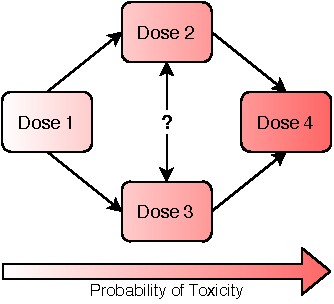
\includegraphics[width=0.75\textwidth]{Adept-DoseExample}
\end{figure}

Wages et al. \cite{wagesContinualReassessmentMethod2011, wagesUsingTimetoeventContinual2013} further developed their work on the PO-CRM to deal with late-onset toxicities by implementing a TITE component. This trial design, referred to as the time-to-event continual reassessment method in the presence of partial orders (PO-TITE-CRM) by the authors, was chosen to be used in ADePT-DDR. A search of PubMed, conducted on the 25th of July 2020, found six articles that had cited the PO-TITE-CRM design by Wages et al. \cite{wagesUsingTimetoeventContinual2013}. Of these six articles non actually implement the design into a trial. The following paragraphs provide more details. 

Five of these papers were methodological in nature, two of which only include the PO-TITE-CRM design in a brief introduction to current methodology before going on to present new Bayesian trial designs \cite{liuBAYESIANDATAAUGMENTATION2013, wheelerBayesianModelfreeApproach2019}. The other three papers were authored by Wages. The first of which details practical considerations and specifications for the PO-CRM design, the TITE variant is only cited as the source of an example which is being used \cite{wagesSpecificationsContinualReassessment2013}. One paper presents an R package 'pocrm' \cite{wagesPocrmRpackagePhase2013, wagesPocrmDoseFinding2019}. The package is only capable of analysing the PO-CRM design. The TITE variant is only referenced here as it illustrates the issue of partial ordering. The last methodological paper by Wages et al. \cite{wagesPracticalDesignsPhase2016} presents three different methods for phase \RN{1} studies of drug combinations one of which is the PO-CRM however, PO-TITE-CRM is only mentioned as an extension to this design. A key message in this paper is the fact that novel methodologies are constantly emerging but are rarely implemented in practice. 

The last paper is a protocol paper for a phase \RN{1}/\RN{2} study, OLA-TMZ-RTE-01 \cite{lesueurPhaseIIaStudy2019}. The phase \RN{1} component of the study aims to determine the recommended phase \RN{2} dose (RP2D) of olaparib combined with a standard schedule of radiotherapy and temozolomide (TMZ) as first line treatment for patients with unresectable glioblastoma (GBM). The treatment schedule is divided into a radiotherapy and maintenance period. They propose to conduct two sequential dose-escalations of seven different  olaparib dose-levels. Patients in the first escalation will be allocated to a dose level of olaparib for 10 weeks including radiotherapy for six weeks with TMZ given each day during radiotherapy and then for six cycles four weeks post radiotherapy during the maintenance period. They state the MTD1 will be determined using a TITE-CRM. Patients in the second escalation olaparib at the MTD1 during the radiotherapy period along with the same schedule of radiotherapy and TMZ. Those patients will then be allocated to one of the seven dose levels of olaparib during the maintenance period. Again, it is stated that the MTD2 will be determined using TITE-CRM modelling. The RP2D is the MTD1 and MTD2 during the radiotherapy and maintenance period respectively. Even though a combination of treatments is being investigated only olaparib is being escalated and doses for other treatments are fixed for all patients. Furthermore, the dose-levels for olaparib increase consistently in either amount or duration meaning there are no issues of partial ordering which would warrant the use of PO-TITE-CRM. The authors reference the TITE-CRM methodology with two papers. One of them being the paper detailing the PO-TITE-CRM design and the other being a paper by Huang and Kuan \cite{huangTimetoeventContinualReassessment2014} which proposes an adaptive weight function that incorporates cyclical data of treatment into the TITE-CRM. It is unclear as to why the PO-TITE-CRM is cited as its methodology is not mentioned anywhere in methods.       

This is just a brief review of the current literature but it seems that the PO-TITE-CRM has rarely been used or discussed since its inception. 

This chapter provides novel insight into the methodology of PO-TITE-CRM through application in a real-world scenario. Section \ref{adept:PO-TITE-CRM-Design} will detail how the PO-TITE-CRM works. Section \ref{adept:PO-TITE-CRM-in-Adept} discusses the justification for implementing the design into the ADePT-DDR trial and our experiences doing so. Section \ref{adept:Exploring-other-designs} explores other alternative designs which could have been implemented and assess how they perform in comparison to the PO-TITE-CRM. We provide some discussion in Section \ref{adept:Discussion} and finally some conclusions in Section \ref{adept:Conclusion}.

%----------------------------------------------------------------------------------------
%	SECTION 2
%----------------------------------------------------------------------------------------
\section{The PO-TITE-CRM Design}
\label{adept:PO-TITE-CRM-Design} 

Wages et al. \cite{wagesUsingTimetoeventContinual2013} introduced the PO-TITE-CRM design which builds directly upon the PO-CRM design by incorporating a TITE component into the dose toxicity model. The aim of which is to determine the target dose for combinations of drugs where the monotonicity assumption does not hold, in a setting where late-onset toxicities are possible.

\begin{table}[h!]
	\centering
	\caption[Example drug combinations with two agents.]{Example of drug combinations for a trial investigating two agents.}
	\label{tab_adept:ex_drug_combo}
	\begin{tabular}{lcccccc}
		\hline  & \multicolumn{6}{c}{\textbf{Drug combinations}}  \\
		\textbf{Agent} & $d_{1}$ & $d_{2}$ & $d_{3}$ & $d_{4}$ & $d_{5}$ & $d_{6}$ \\ \hline
		A (mg/day) & 0.25 & 0.5 & 1.0 & 0.25 & 0.5 & 1.0         \\
		B (mg/day) & 1.0  & 1.0 & 1.0 & 1.5  & 1.5 & 1.5         \\ \hline
	\end{tabular}
\end{table}

To help understand partial ordering, consider an example of an early phase trial investigating the combination of two agents. Drug A which consists of three doses (0.25, 0.5, 1.0 mg/day) and drug B which consists of two doses (1.0, 1.5 mg/day), for a total of six drug combinations $d_{1}$, ..., $d_{6}$ (Table \ref{tab_adept:ex_drug_combo}). For each drug independently we assume they have a monotonic dose-toxicity curve however, the ordering of toxicity probabilities for some of the treatment combinations is unknown. Specifically, we can say $d_{1}$ is less toxic than $d_{2}$ as the dose of drug A increased whilst the dose of drug B stayed the same. This is also the case for $d_{2}$ and $d_{3}$. So, $d_{1}$ can always be considered less toxic than $d_{2}$ which is always less toxic than $d_{3}$. The same can be said for doses $d_{4}$, $d_{5}$ and $d_{6}$, these three doses are can also all be considered more toxic than $d_{1}$ as well.The order between $d_{4}$ and $d_{5}$ in comparison to $d_{3}$ is not known because the dose of drug A decreases whilst the dose of drug B increases. Similarly the order between $d_{2}$ and $d_{4}$ is unknown. Also, we can say that $d_{6}$ is the always the most toxic dose. Assessing all these potential order toxicity relationships leaves five possible orderings. 

\begin{enumerate}
	\centering
	\item $d_{1} \rightarrow d_{2} \rightarrow d_{3} \rightarrow d_{4} \rightarrow d_{5} \rightarrow d_{6}$
	\item $d_{1} \rightarrow d_{2} \rightarrow d_{4} \rightarrow d_{3} \rightarrow d_{5} \rightarrow d_{6}$
	\item $d_{1} \rightarrow d_{2} \rightarrow d_{4} \rightarrow d_{5} \rightarrow d_{3} \rightarrow d_{6}$
	\item $d_{1} \rightarrow d_{4} \rightarrow d_{2} \rightarrow d_{3} \rightarrow d_{5} \rightarrow d_{6}$
	\item $d_{1} \rightarrow d_{4} \rightarrow d_{2} \rightarrow d_{5} \rightarrow d_{3} \rightarrow d_{6}$
\end{enumerate}


Using the notation of Wages et al. \cite{wagesContinualReassessmentMethod2011,wagesUsingTimetoeventContinual2013}, let $M$ denote the number of possible orders and $Y$ be an indicator of a toxicity event. Then for a trial investigating $k$ combinations, $d_{1}$,...,$d_{k}$, the dose for the $j$th patient, $X_{j}$, $j$ = 1,...,$n$ can be thought of as random $x_{j} \in (d_{1}, ..., d_{k})$. For a specific ordering $m$, $m = 1,...,M$ the toxicity probability $R(d_{i})$ is modelled by 
\begin{equation}
R(d_{i}) =  \phi_m(d_i,w,\beta) = w\psi_m(d_i,\beta) \; i = 1, ..., k; \; m = 1, ...,M
\end{equation}
for  a weighted dose response model $\phi_m(d_i,w,\beta)$ where $\beta \in (-\infty, \infty)$. The weight, $w$ as defined by Cheung and Chappel \cite{cheungSequentialDesignsPhase2000}, is a function of the time-to-event of each patient and is incorporated linearly with the dose toxicity model $\psi$ so that $0 \leq w \leq 1$. Each patient is followed for a fixed amount of time $T$. Let $U_j$ represent the time-to-toxicity of patient $j$. Then for $u \leq T$, 
\begin{equation}
	P(U_j \leq u ) = P(U_j \leq u |U_j \leq T)P(U_j \leq T) \equiv w(u;T) \psi_m(d_i,\beta).
\end{equation}
For simplicity we will refer to the weight function $w(u;T)$ as $w$. The weight function will have to be decided upon by the trials team, dependent on the scenario, a simple linear function or a more complex adaptive weights function could be utilised. There are also several working dose models which could be used for $\psi$, Wages et al. \cite{wagesUsingTimetoeventContinual2013} present their design with the power parameter model given by 
\begin{equation}
	\psi_m(d_i,\beta) = \alpha_{mi}^{exp(\beta)} \; i = 1,...,k; \; m = 1,...,M.
\end{equation}
Here $0 < \alpha_{m1} < ... < \alpha_{mk} < 1$ are the prior estimates of toxicity probabilities, or skeleton, for each potential ordering. Furthermore, prior probabilities are assigned to each order $M$ to account for any prior information regarding the plausibility of each model such that, $p(m) = \{p(1),...,p(M)\}$, where $p(m) \geq 0$ and $\sum_mp(m)=1$. When all orders are equally likely or there is no prior information available on possible orderings the prior is discretely uniform and would be $p(m) = 1/M$. 

A Bayesian framework is used and a prior probability distribution $g(\beta)$ is assigned to the parameter $\beta$. The ordering with the largest prior probability is selected as the starting ordering, in the scenario where all priors are equal an ordering is selected at random, subsequently a starting dose is also chosen. After $j$ patients have been entered into the trial data is collected in the form of $\Omega_j = \{x_1,y_1, ..., x_j,y_j\}$. A weighted likelihood for the parameter $\beta$ is used to establish running probabilities of toxicity for each treatment combination. The weighted likelihood under ordering $m$, is given by 
\begin{equation}
\label{eq_adept:likelihood}
\tilde{L}_m(\beta|\Omega_j)=\prod_{l=1}^{j}\phi_m^{y_l}(x_l,w_l,\beta)\{1-\phi_m(x_l,w_l,\beta)\}^{(1-y_l)}
\end{equation} 
which can be used to generate a summary value $\hat{\beta}_{mj}$ for each ordering. With the likelihood and the data $\Omega_j$, the posterior density for $\beta$ can be calculated using 
\begin{equation}
	\tilde{f}_m(\beta|\Omega_j)=\frac{\tilde{L}_m(\beta|\Omega_j)g(\beta)}{\int_{\beta}\tilde{L}_m(\beta|\Omega_j)g(\beta)d\beta}
\end{equation}
This can then be used to establish posterior probabilities of the orderings given the data as 
\begin{equation}
\tilde{\pi}(m|\Omega_j)=\frac{p(m)\int_{\beta}\tilde{L}_m(\beta|\Omega_j)g(\beta)d\beta}{\sum_{m=1}^{M}p(m)\int_{\beta}\tilde{L}_m(\beta|\Omega_j)g(\beta)d\beta}.
\end{equation}
We select the single ordering, $h$, with the largest posterior probability along with its associated working model $\psi_h(d_i,\beta)$ and generate toxicity probabilities for each dose level. Once the $j$th patient has been included the posterior probability of DLT can be calculated for $d_{i}$ so that
\begin{equation}
	\hat{R}(d_i) = \psi_h(d_i,\hat{\beta}_{hj}); \; \hat{\beta}_h = \int_{\beta}\beta\tilde{f}_h(\beta|\Omega_j)d\beta.
\end{equation}

In turn, the dose level $x_j \in \{d_1,...,d_k\}$ assigned to the ($j+$1)th patient is the dose, $d_i$, which minimises 
\begin{equation}
\label{eq_adept:crm_min}
	\triangle(\hat{R}(d_i),\theta) = |\hat{R}(d_i)-\theta|, \; i=1,...,k
\end{equation}
where $\theta$ is the target toxicity rate. Similarly, once all patients have been recruited and observed and the trial ends, the target dose (TD$\theta$) is the dose, $d_{i}$, which minimises (\ref{eq_adept:crm_min}).

%----------------------------------------------------------------------------------------
%	SECTION 3
%-------------------------.

\section{PO-TITE-CRM in ADePT-DDR}  
\label{adept:PO-TITE-CRM-in-Adept}

The decision to implement PO-TITE-CRM into ADePT-DDR was made by Piers Gaunt (PG) after discussions with other statisticians Kristian Brock (KB) and Daniel Slade (DS), as well as the chief investigator and other co-investigators. The design was chosen as the toxicity probabilities of the dose levels weren't monotonically increasing which restricts the use of most early phase designs such as the CRM. Additionally, the design also handles late-onset toxicities which would be an issue in ADePT-DDR due to the treatment involving radiotherapy. The availability of software to conduct the trial was also a factor that was considered. The R package 'pocrm' \cite{wagesPocrmRpackagePhase2013} only provides a means for implementing the PO-CRM design but the easy accessibility to this code meant that it could be extended to include the TITE component.  

The intended use of this design is for dose-finding in combinations of therapies, as this is the source of the partial ordering issue. ADePT-DDR however, is a unique implementation of the design as even though it involves a combination of therapies (radiotherapy and AZD6783) the dose of radiotherapy is fixed and dose-finding is only planned for AZD6783. PO-TITE-CRM is still applicable in this case as the design includes combinations of dose and duration for AZD6783 which are partially ordered. 

A two-stage PO-TITE-CRM will be used to find the TD25 of AZD6783. This will be determined by dose-limiting toxicities evaluated by Common Terminology Criteria for Adverse Events (CTCAE) v5.0 and Radiation Therapy Oncology Group (RTOG) late toxicity score. The binary DLT events are pre-defined by a variety of grade 3-4 adverse events notably, haematological, cardiovascular and gastrointestinal/hepatic toxicities as well as significant non-haematological events and specific treatment-related toxicities. DLTs will be monitored for the duration of treatment (seven weeks) and throughout the follow-up period. The total follow-up period post treatment is 52 weeks, so patients will spend a total of 59 weeks in the trial.  

A maximum of 60 patients will be recruited for the dose-finding aspect of this trial and up to 20 patients as controls. Controls will be utilised to make comparisons for secondary outcomes such as survival and efficacy. Control patients will only be receiving radiotherapy, the dose of which is fixed at 70Gy/35F. Cohorts of three patients will be recruited and assigned to dose levels chosen by the PO-TITE-CRM. Controls will be recruited in the interim period between the recruitment of the third patient in a cohort and the completion of the minimum follow-up period.    

%-----------------------------------
%	SUBSECTION 3.1
%-----------------------------------
\subsection{Partial Ordering in Practice}
\label{adept:Partial-ordering-in-practice}%first number is the chapter number, second number is section number, third is subsection etc..

Each patient entered into ADePT-DDR will receive fixed dose radiation, totalling 70 Gy in 35 fractions over seven weeks. For the dose-finding aspect we investigate six doses of AZD6783 detailed in table \ref{tab_adept:AZD_dose_levels}. Treatment dose and duration to be selected for dose level 3 will be determined based on a combination of data observed, adverse events and compliance. The issue of partial ordering is illustrated in Figure \ref{fig_adept:AZD_dose_levels} inspired from plots by Wages et al. \cite{wagesUsingTimetoeventContinual2013}. The doses to be used in this trial are detailed in their appropriate box. Additionally, each dot represents a potential dose combination which theoretically could be investigated. The combinations are colour coordinated to indicate where partial ordering exists in this dose combination space. Doses across the same colour (each diagonal) cannot be distinguished from each other in terms of probability of toxicity. However, it forms a hierarchy in which doses of the same colour can be thought of as less/more toxic that doses in another colour i.e the red dose levels would have a higher probability of toxicity than the yellow dose levels. It is clear that dose levels 2a and 2b would be considered more toxic than dose level 1 due to the increase in treatment duration and treatment dose respectively. When comparing 2a and 2b it is unknown whether the increase in dose or duration will be more toxic. Hence there are two possible orderings for ADePT-DDR. 

\begin{enumerate}
	\centering
	\item $d_{-1} \rightarrow d_{0} \rightarrow d_{1} \rightarrow d_{2a} \rightarrow d_{2b} \rightarrow d_{3}$
	\item $d_{-1} \rightarrow d_{0} \rightarrow d_{1} \rightarrow d_{2b} \rightarrow d_{2a} \rightarrow d_{3}$
\end{enumerate}

\begin{table}[h!]
    \centering
	\caption[ADePT-DDR dose-levels.]{ADePT-DDR dose-levels and duration of treatment for AZD6783.}
	\label{tab_adept:AZD_dose_levels}
		\begin{tabular}{ccccc}
			\hline 
			\multicolumn{1}{p{1.5cm}}{\centering \textbf{Dose} \\ \textbf{Level}} & \multicolumn{1}{p{3cm}}{\centering \textbf{AZD6783 Daily} \\ \textbf{dose (mg BD)}} &
		    \multicolumn{1}{p{1.5cm}}{\centering \textbf{Weeks} \\ } &
			\multicolumn{1}{p{1.5cm}}{\centering \textbf{Duration} \\ \textbf{(days)}} &
			\multicolumn{1}{p{3.5cm}}{\centering \textbf{Radiotherapy} \\ } 
			\\\hline
			-1 & 20 & 1 & 5 & 70 Gy/ 35 F \\
			 0 & 20 & 1\&4 & 10 & 70 Gy/ 35 F \\
			 1 & 40 & 1\&4 & 10 & 70 Gy/ 35 F \\
			2a & 40 & 1,2,4\&5 & 20 & 70 Gy/ 35 F \\
			2b & 80 & 1\&4 & 10 & 70 Gy/ 35 F \\
			\multirow{2}{*}{3} & 120 & 1\&4 & 10 & 70 Gy/ 35 F \\
			& 80 & 1,2,4\&5 & 20 & 70 Gy/ 35 F \\ \hline
		\end{tabular}
\end{table}

\begin{figure}[h!]
	\centering
	\caption{ADePT-DDR dose levels across dose and duration.}
	\label{fig_adept:AZD_dose_levels}
	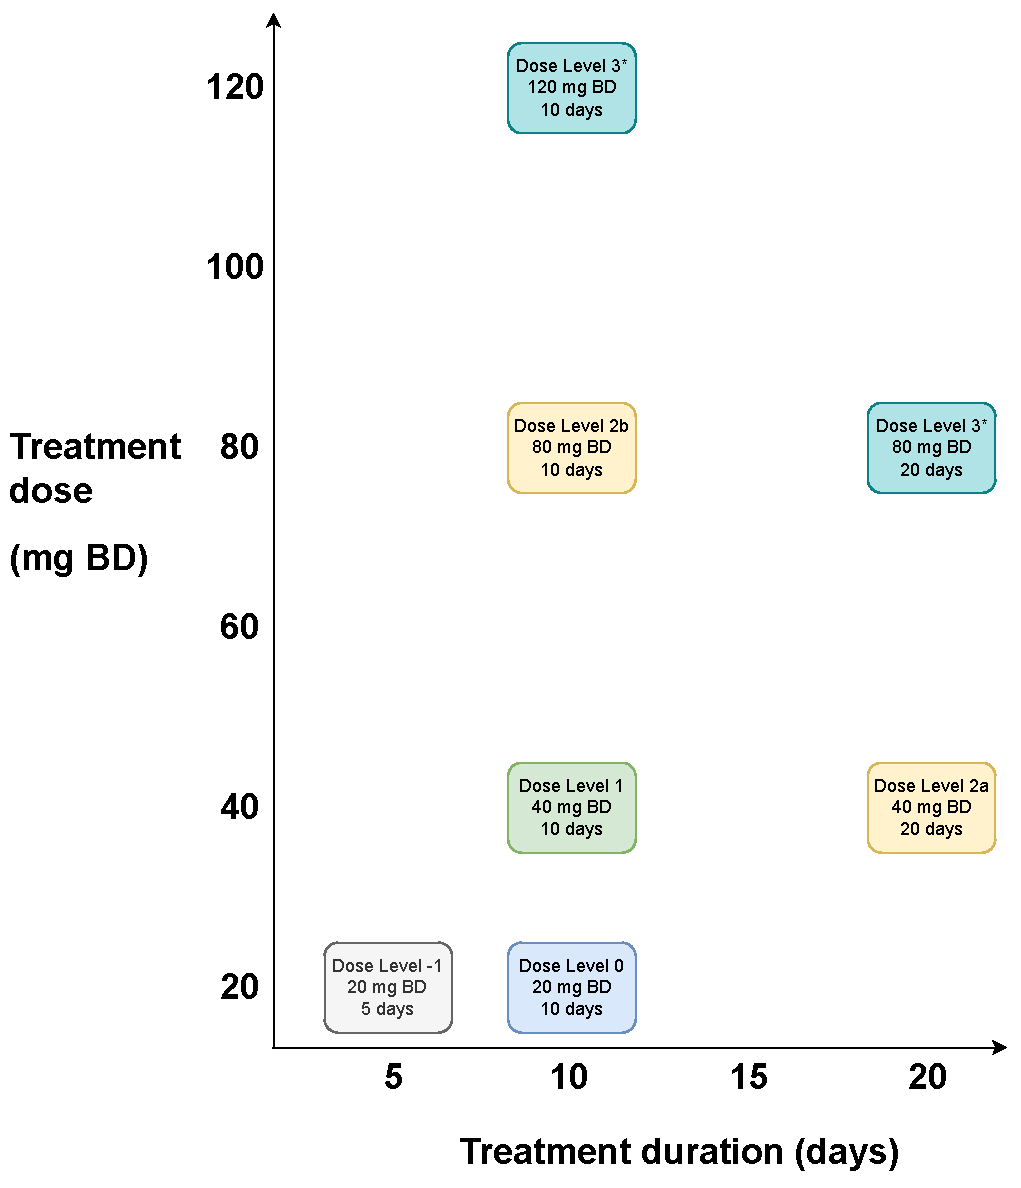
\includegraphics[width=\textwidth]{Adept-DoseCombos}
\end{figure}

Traditionally, dose-finding trials for combinations would select dose levels to form a 'path' through the dose combination space such that each subsequent dose level was logically more toxic. This avoids the issue of partial ordering but means doses of interest or effective dose combinations may be missed or not investigated. Specifically, for ADePT-DDR this allows two 'paths' from dose level 1 extending to 2a and 2b. In terms of dose level 3 only one of the doses in that tier will be investigated, it was unclear as to which dose level would be best due to a lack of historical data. Even though dose level 3 is not yet specified in terms of modelling and simulations it was treated as singular dose. This was done as clinicians thought that it would be unlikely that we'd reach these doses and that the probability of toxicity between them would be similar.  

Preliminary designs of the trial included only five dose levels and planned to use dose level 0 as the starting dose. During the trial design phase it was decided a new lower dose (dose level -1) would be introduced to allow for de-escalation if the initial dose was found to be too toxic. Dose escalation/de-escalation for subsequent cohorts would be determined from the two-stage PO-TITE-CRM. A two-stage design allows for escalation according to a pre-defined escalation scheme similar to a '3+3' design. The first stage dictates that if no DLT's are observed in the current cohort the dose allocated to the next cohort is the following dose in the escalation scheme. Dose levels continue to be incremented in this fashion until the first DLT is observed. In stage two, dose levels are determined by the PO-TITE-CRM.

Typically CRM designs begin by testing the first patient, or cohort, at the prior guess of TD or at a lower dose to be safe. However, clinicians may have safety concerns beginning the trial at higher dose levels as well as escalating to higher dose levels without testing lower ones. Investigators in ADePT-DDR expressed similar concerns as such a two-stage design was adopted. The escalation scheme used in stage one of ADePT-DDR will follow that of the first ordering ($d_{-1} \rightarrow d_{0} \rightarrow d_{1} \rightarrow d_{2a} \rightarrow d_{2b} \rightarrow d_{3}$). If patients in the first cohort (assigned to dose level 0) don't experience a DLT the next cohort will be allocated to dose level 1 and then if no DLTs are observed again the third cohort will be allocated to dose level 2a and so on and so forth. The dose escalation scheme was determined based on the prior probabilities of toxicity generated for each dose level.  

Information elicited from the investigators helped generate prior probabilities of toxicity for each dose level. They believed that dose level 2b would be the TD25 with 2a being less toxic. This was used in conjunction with the getprior function from the dfcrm R package \cite{cheungDfcrmDoseFindingContinual2019} which yielded priors of 0.012, 0.036, 0.084, 0.157, 0.25 and 0.355 for dose levels -1, 0, 1, 2a, 2b and 3 respectively. The half-width of the indifference interval was set at 0.05. The indifference interval is an interval in which the toxicity probability of the selected dose will eventually fall. Prior probabilities are also required for the plausibility of each model and even though the clinicians think that 2b will be more toxic than 2a there is no clear evidence and still a lot of uncertainty. As such it is sensible to assume a plausibility probability of 0.5 for each ordering, implying both orders are equally likely to be the true ordering of these dose levels. 

%-----------------------------------
%	SUBSECTION 3.2
%-----------------------------------
\subsection{The TITE component}
\label{adept:The-TITE-component}

The observation window for this trial will be up to a year post-treatment as the combination of radiotherapy with AZD6738 is anticipated to cause late-onset toxicity. The Acute DLT observation period is 12 weeks (84 days) post radiotherapy end with a minimum of 8 weeks (56 days) for the last patient of each cohort. However, patients will continuously be monitored for occurrence of DLT for at least12 weeks (84 days), i.e. at least 12 weeks (84 days) from the end of radiotherapy. The full window will last for 52 weeks (365 days) post-treatment.

The TITE component incorporates a weighting contribution for each patient dependent on how long that patient has been evaluable in the study. This allows a patient to be evaluated once they have been observed for the minimum DLT period of 8 weeks (56 days). The weighting at this point is 60\% rising to 80\% at 12 weeks (84 days). A patient will not contribute fully to the model until they have completed 52 weeks (365 days) follow up (or have experienced a DLT at any stage in which case they will be weighted as a whole contribution). Linear weighting functions will be employed for any patient with a length of follow up between these three time points. One weight function to calculate weights between 8-12 weeks and another for weights between 12-52 weeks. For the weighting function $w(u;t_1, t_2, t_3)$ where $u$ is the time-to-toxicity of patient $j$ and $t_1, t_2, t_3$ is the time period with values 8, 12 and 52 respectively. Then for $t_1 \leq u \leq t_3$
\begin{equation}
w(u;t_1,t_2,t_3) = 0.6 + 0.2\frac{min(0, min(u, t_2) - t_1)}{t_2 - t_1} + 0.2\frac{max(0, u - t_2)}{t_3-t_2}.
\end{equation} 
All patients will have a minimum weight of 60\% as that is the prescribed weighting to the  minimum follow up period before dose escalation/de-escalation decisions can be made. For each additional week the patient is observed, without a DLT occurring, between weeks 8 and 12 their weighting increases by 5\%. Similarly for each week between 12 and 52 weeks, without a DLT, weighting increases by 0.5\%. Figure \ref{fig_adept:weight_function} illustrates the weight function and how the weight changes for patients dependent on how long they have been followed-up.   

\begin{figure}[h!]
	\centering
	\caption[Weight function across the follow-up period.]{Weights of patients who have not experienced a DLT across the observation window.}
	\label{fig_adept:weight_function}
	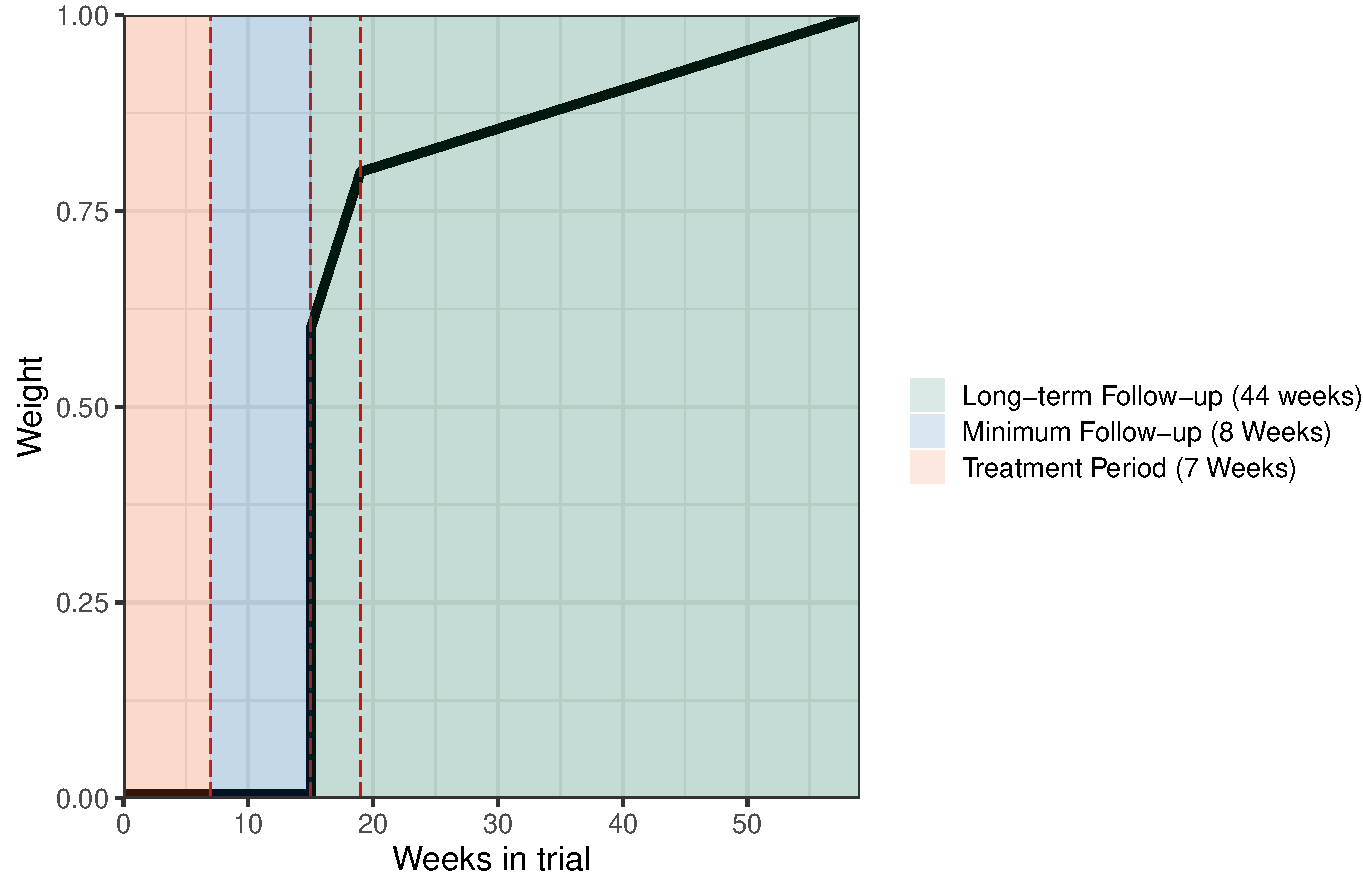
\includegraphics[width=\textwidth]{Adept-WeightFunction}
\end{figure}


The TITE-CRM originally presented by Cheung and Chappel \cite{cheungSequentialDesignsPhase2000} did not incorporate a minimum follow-up period and their design allowed for the continual recruitment of patients whenever they became available. There are some practical considerations which make this infeasible in ADePT-DDR. The model would need to be run each time a new patient entered the study which requires statistical input hence the introduction of cohorts. Clinicians may also have safety concerns if we see rapid recruitment at the start of the trial and the model keeps escalating so we impose a minimum follow-up period. Initially this was set at 12 weeks (at 80\% weighting) however, statisticians AP and PG  pointed out that dose escalation/de-escalation decisions would have to take place 19 weeks (7 weeks treatment and 12 weeks follow-up) after recruitment of the third patient in the cohort. Dependent on the recruitment rates this could extend the duration of the trial and negates the benefits of using a TITE design. The investigators aslo agreed this was too long and settled on lowering this period to 8 weeks (at 60\% weighting) whilst also including the original 12 week weighting of 80\%.


%-----------------------------------
%	SUBSECTION 3.3
%-----------------------------------
\subsection{Stopping Rules}
\label{adept:Stopping-rules}

A practical modification was included to allow for early stopping of the trial if there is sufficient evidence that the TD has been reached. Sufficient evidence is achieved once 15 patients (five cohorts) have been treated at the same dose level and the model allocates that dose level again to a sixth cohort. This rule evolved from the original designs of the trial which involved 30 patients with a dose expansion cohort to ensure at least 15 patients were treated at the TD. 

Initial simulations highlighted the inadequacy of these design parameters as operating characteristics for various scenarios were poor, specifically in terms of correct TD selection. Clinicians explained the inclusion of the dose expansion cohort was to ensure the dose-finding aspect of the trial did not take a large amount of time whilst also allowing safety to be assessed at the TD. In order to ensure that a reasonable amount of patients would be treated at the TD, the trial wouldn't take longer than necessary and operating characteristics improved, the sample size was increase and this rule was introduced.

A rule was also implemented to allow for early termination of the trial in the case of excess toxicity at the lowest dose. If the probability of DLT at the lowest dose is higher than 0.35 with a probability of 80\% and has been tested the trials safety committee will be alerted and will recommend if the trial should be stopped. As the trial starts at dose level 0, which is not the lowest dose, it is possible for the trial to recommend terminating without ever allocating patients to the lowest dose level. As such it was decided early termination would only occur once at least 3 patients (1 cohort) have been allocated dose level -1. 

An approximate estimate of the variance was calculated using methodology presented by O'Quigley and Shen \cite{oquigleyContinualReassessmentMethod1996}. The observed information matrix is obtained by taking the second derivative of the likelihood (eq. \ref{eq_adept:likelihood}) which is then used to calculate the variance $v(\hat{\beta_j})$, for estimate $\beta_j$ which becomes more accurate with larger sample sizes. After each cohort, we sample many times from a normal distribution with parameters based on the estimate of $\beta_j$ and its variance. These samples are then plugged into our dose-toxicity model to ascertain the probability of toxicity at the lowest dose. The trial will be recommended to stop if it breaks the rule based on the criteria above. 


%-----------------------------------
%	SUBSECTION 3.4 
%-----------------------------------
\subsection{Operating Characteristics}
\label{adept:OCs} 

Simulations were continually utilised during the design process of the trial to assess how various changes impact the overall performance. These changes to design features such as the sample size, weight function and stopping rules helped inform decisions which led to the final design.  

Functions from pocrm package in R \cite{wagesPocrmRpackagePhase2013, wagesPocrmDoseFinding2019} were modified in order to perform simulations and conduct the trial. The majority of work involved integrating the TITE component and the stopping rules into the code. In standard CRM designs a binary outcome for toxicity is generated for each patient based on a pre-specified true DLT rates for the dose they are assigned. Adding the TITE component means the time the toxicity occurs also has to be generated, the simulation must also track this time and incorporate this information into the PO-TITE-CRM model when it needs to make dose allocation decisions for the next cohort. We defined multiple scenarios to reflect various real life possibilities in order to assess the designs performance.  

Standard scenarios to run involve adjusting the true DLT rates to reflect each dose being the TD25. For each of these we calculate the probability of selecting each dose as the TD25. It would be expected the dose with the highest probability of being selected has its true DLT rate set at 25\% to match the target rate. A high probability of selection for the correct dose implies the design works well in the specified scenario. Additional characteristics such as the average number of patients at each dose level are also investigated. This can be used to look at how many patients may potentially be allocated to a toxic dose. It is also necessary to consider performance when all doses are too toxic, here we would want the design to recommend stopping early. Usually the true DLT rates used to define these scenarios abide by the monotonicity assumption. Due to the partial ordering we consider scenarios in which the true DLT rates follow both orders. For trials with a large amount of orders it may be unfeasible to run so many simulations. However, as ADePT-DDR only has two orders we explored all scenarios for each ordering.

We simulated 10000 trials for each scenario using the finalised design detailed in section \ref{adept:PO-TITE-CRM-in-Adept}. Simulations were based on the assumption that the trial would recruit one patient per month. The occurrence of DLT's were randomly generated for patients in each cohort using a Bernoulli distribution with the probability set at the true DLT rate for the cohorts assigned dose level in the specific scenario. For patients who had a DLT occur, the time at which the DLT occurred was randomly generated using a uniform distribution which spanned the start of treatment to the end of follow-up. The simulations presented in Tables \ref{tab_adept:OCorder1} and \ref{tab_adept:OCorder2} took approximately 5 hours and 53 minutes to run. The Monte Carlo standard error for probabilities estimated by 10000 simulations is $\sqrt{0.5 \times 0.5/10000} = 0.5\%$.

Table \ref{tab_adept:OCorder1} details simulations for eight scenarios to test the performance of the PO-TITE-CRM design using true DLT rates which reflect the first ordering. We analyse scenarios where each dose is the TD25 (scenarios 1-6) and when all doses are too toxic (scenario 8). Additionally, we also investigate performance under conditions where the probability of DLT is fairly similar between doses (scenario 7). This is a notoriously difficult circumstance for CRM designs to deal with as the limited number of patients and events at each dose make it hard to accurately estimate toxicity probabilities if they are similar. Simulation results for ordering 2 are shown in Table \ref{tab_adept:OCorder2} where dose level 2a is considered more toxic than 2b. This is achieved by altering the true DLT rates so 2b has a lower probability of DLT compared to 2a. 

Ideally we want the probability of selection for the dose allocated at TD25 to be as high as possible and greater than other dose levels. For scenarios 1-7 the TD25 is highlighted in bold along with results from the simulations. However, for scenario 8 where all doses are too toxic we expect the trial to terminate early, here 'stop' should be selected and its associated probability of stopping is shown in bold. 

\begin{table}[h!] % OC for order 1 
	
	\caption[Operating Characteristics for ordering 1.]{\label{tab_adept:OCorder1} Operating Characteristics of the two-stage PO-TITE-CRM (with true DLT rates that imply 2b is more toxic than 2a) based on 10000 simulated trials. Definitions: DLT: Dose-limiting toxicity. P(select):
		Probability of selecting a dose as the TD25.}
	\centering
	\begin{singlespace}
		\resizebox{\linewidth}{!}{
			\begin{tabular}[t]{ccccccccc}
				\toprule
				\multicolumn{2}{c}{ } & \multicolumn{6}{c}{Dose Levels} \\
				\cmidrule(l{3pt}r{3pt}){3-8}
				&  & -1 & 0 & 1 & 2a & 2b & 3 & Stop\\
				\midrule
				Scenario & Prior DLT & 0.01 & 0.04 & 0.08 & 0.16 & 0.25 & 0.35 & \\
				\cmidrule{1-9}
				\rowcolor{gray!6}   & True DLT rate & 0.25 & 0.4 & 0.45 & 0.5 & 0.55 & 0.6 & \\
				
				\rowcolor{gray!6}   & P(select) & 0.68 & 0.18 & 0.05 & 0.01 & 0 & 0 & 0.0849\\
				
				\rowcolor{gray!6}   & \% of patients & 39 & 32 & 20 & 6 & 3 & 0 & \\
				
				\rowcolor{gray!6}  \multirow{-4}{*}{\centering\arraybackslash 1: TD25 @-1} & Mean number of patients & 10.17 & 8.46 & 5.33 & 1.67 & 0.69 & 0.07 & \\
				\cmidrule{1-9}
				& True DLT rate & 0.12 & 0.25 & 0.4 & 0.45 & 0.5 & 0.55 & \\
				
				& P(select) & 0.23 & 0.51 & 0.2 & 0.03 & 0.02 & 0 & 0.0079\\
				
				& \% of patients & 17 & 35 & 29 & 11 & 6 & 1 & \\
				
				\multirow{-4}{*}{\centering\arraybackslash 2: TD25 @0} & Mean number of patients & 5.24 & 10.48 & 8.75 & 3.4 & 1.83 & 0.26 & \\
				\cmidrule{1-9}
				\rowcolor{gray!6}   & True DLT rate & 0.09 & 0.12 & 0.25 & 0.4 & 0.45 & 0.5 & \\
				
				\rowcolor{gray!6}   & P(select) & 0.02 & 0.2 & 0.55 & 0.14 & 0.09 & 0.01 & 4e-04\\
				
				\rowcolor{gray!6}   & \% of patients & 4 & 20 & 34 & 23 & 16 & 3 & \\
				
				\rowcolor{gray!6}  \multirow{-4}{*}{\centering\arraybackslash 3: TD25 @1} & Mean number of patients & 1.22 & 6.41 & 10.97 & 7.23 & 5.14 & 1.02 & \\
				\cmidrule{1-9}
				& True DLT rate & 0.06 & 0.09 & 0.12 & 0.25 & 0.4 & 0.45 & \\
				
				& P(select) & 0 & 0.02 & 0.22 & 0.48 & 0.23 & 0.05 & 1e-04\\
				
				& \% of patients & 1 & 12 & 20 & 31 & 25 & 11 & \\
				
				\multirow{-4}{*}{\centering\arraybackslash 4: TD25 @2a} & Mean number of patients & 0.47 & 3.88 & 6.74 & 10.43 & 8.2 & 3.5 & \\
				\cmidrule{1-9}
				\rowcolor{gray!6}   & True DLT rate & 0.03 & 0.06 & 0.09 & 0.12 & 0.25 & 0.4 & \\
				
				\rowcolor{gray!6}   & P(select) & 0 & 0 & 0.02 & 0.3 & 0.43 & 0.25 & 0\\
				
				\rowcolor{gray!6}   & \% of patients & 1 & 10 & 12 & 24 & 28 & 25 & \\
				
				\rowcolor{gray!6}  \multirow{-4}{*}{\centering\arraybackslash 5: TD25 @2b} & Mean number of patients & 0.25 & 3.36 & 4.15 & 8.17 & 9.33 & 8.33 & \\
				\cmidrule{1-9}
				& True DLT rate & 0.01 & 0.03 & 0.06 & 0.09 & 0.12 & 0.25 & \\
				
				& P(select) & 0 & 0 & 0 & 0.09 & 0.13 & 0.78 & 0\\
				
				& \% of patients & 0 & 10 & 11 & 18 & 18 & 42 & \\
				
				\multirow{-4}{*}{\centering\arraybackslash 6: TD25 @3} & Mean number of patients & 0.1 & 3.13 & 3.49 & 5.46 & 5.6 & 13.14 & \\
				\cmidrule{1-9}
				\rowcolor{gray!6}   & True DLT rate & 0.05 & 0.1 & 0.15 & 0.2 & 0.25 & 0.3 & \\
				
				\rowcolor{gray!6}   & P(select) & 0 & 0.03 & 0.12 & 0.31 & 0.28 & 0.26 & 3e-04\\
				
				\rowcolor{gray!6}   & \% of patients & 2 & 13 & 18 & 26 & 23 & 19 & \\
				
				\rowcolor{gray!6}  \multirow{-4}{*}{\centering\arraybackslash 7: Equal steps in DLT rate} & Mean number of patients & 0.55 & 4.03 & 5.72 & 8.32 & 7.15 & 5.96 & \\
				\cmidrule{1-9}
				& True DLT rate & 0.5 & 0.6 & 0.65 & 0.7 & 0.75 & 0.8 & \\
				
				& P(select) & 0.26 & 0 & 0 & 0 & 0 & 0 & 0.7404\\
				
				& \% of patients & 56 & 26 & 15 & 2 & 0 & 0 & \\
				
				\multirow{-4}{*}{\centering\arraybackslash 8: All  toxic} & Mean number of patients & 9.05 & 4.27 & 2.4 & 0.37 & 0.04 & 0 & \\
				\bottomrule
			\end{tabular}
		}
	\end{singlespace}
\end{table}

\begin{table}[h!] % OC for order 2
	
	\caption[Operating Characteristics for ordering 2.]{\label{tab_adept:OCorder2}  Operating Characteristics of the two-stage PO-TITE-CRM (with true DLT rates that imply 2a is more toxic than 2b) based on 10000 simulated trials. Definitions: DLT: Dose-limiting toxicity. P(select): Probability of selecting a dose as the TD25.}
	\centering
	\begin{singlespace}
		\resizebox{\linewidth}{!}{
			\begin{tabular}[t]{ccccccccc}
				\toprule
				\multicolumn{2}{c}{ } & \multicolumn{6}{c}{Dose Levels} \\
				\cmidrule(l{3pt}r{3pt}){3-8}
				&  & -1 & 0 & 1 & 2a & 2b & 3 & Stop\\
				\midrule
				Scenario & Prior DLT & 0.01 & 0.04 & 0.08 & 0.16 & 0.25 & 0.35 & \\
				\cmidrule{1-9}
				\rowcolor{gray!6}   & True DLT rate & 0.25 & 0.4 & 0.45 & 0.55 & 0.5 & 0.6 & \\
				
				\rowcolor{gray!6}   & P(select) & 0.67 & 0.19 & 0.05 & 0 & 0.01 & 0 & 0.0827\\
				
				\rowcolor{gray!6}   & \% of patients & 39 & 32 & 20 & 6 & 3 & 0 & \\
				
				\rowcolor{gray!6}  \multirow{-4}{*}{\centering\arraybackslash 9: TD25 @-1} & Mean number of patients & 10.19 & 8.43 & 5.27 & 1.6 & 0.68 & 0.07 & \\
				\cmidrule{1-9}
				& True DLT rate & 0.12 & 0.25 & 0.4 & 0.5 & 0.45 & 0.55 & \\
				
				& P(select) & 0.23 & 0.52 & 0.2 & 0.02 & 0.02 & 0 & 0.0074\\
				
				& \% of patients & 18 & 36 & 29 & 11 & 6 & 1 & \\
				
				\multirow{-4}{*}{\centering\arraybackslash 10: TD25 @0} & Mean number of patients & 5.24 & 10.64 & 8.82 & 3.16 & 1.85 & 0.24 & \\
				\cmidrule{1-9}
				\rowcolor{gray!6}   & True DLT rate & 0.09 & 0.12 & 0.25 & 0.45 & 0.4 & 0.5 & \\
				
				\rowcolor{gray!6}   & P(select) & 0.02 & 0.2 & 0.55 & 0.09 & 0.14 & 0.01 & 4e-04\\
				
				\rowcolor{gray!6}   & \% of patients & 4 & 20 & 34 & 21 & 17 & 3 & \\
				
				\rowcolor{gray!6}  \multirow{-4}{*}{\centering\arraybackslash 11: TD25 @1} & Mean number of patients & 1.16 & 6.43 & 11.07 & 6.83 & 5.6 & 1.07 & \\
				\cmidrule{1-9}
				& True DLT rate & 0.06 & 0.09 & 0.12 & 0.25 & 0.15 & 0.45 & \\
				
				& P(select) & 0 & 0.01 & 0.08 & 0.44 & 0.33 & 0.14 & 2e-04\\
				
				& \% of patients & 1 & 11 & 16 & 30 & 24 & 18 & \\
				
				\multirow{-4}{*}{\centering\arraybackslash 12: TD25 @2a} & Mean number of patients & 0.48 & 3.78 & 5.24 & 10.1 & 7.9 & 6.07 & \\
				\cmidrule{1-9}
				\rowcolor{gray!6}   & True DLT rate & 0.03 & 0.06 & 0.09 & 0.35 & 0.25 & 0.4 & \\
				
				\rowcolor{gray!6}   & P(select) & 0 & 0 & 0.15 & 0.31 & 0.43 & 0.11 & 0\\
				
				\rowcolor{gray!6}   & \% of patients & 1 & 11 & 18 & 30 & 28 & 14 & \\
				
				\rowcolor{gray!6}  \multirow{-4}{*}{\centering\arraybackslash 13: TD25 @2b} & Mean number of patients & 0.25 & 3.5 & 5.9 & 9.82 & 9.14 & 4.54 & \\
				\cmidrule{1-9}
				& True DLT rate & 0.01 & 0.03 & 0.06 & 0.12 & 0.09 & 0.25 & \\
				
				& P(select) & 0 & 0 & 0 & 0.13 & 0.09 & 0.78 & 0\\
				
				& \% of patients & 0 & 10 & 11 & 19 & 16 & 43 & \\
				
				\multirow{-4}{*}{\centering\arraybackslash 14: TD25 @3} & Mean number of patients & 0.1 & 3.13 & 3.51 & 5.88 & 5.06 & 13.13 & \\
				\cmidrule{1-9}
				\rowcolor{gray!6}   & True DLT rate & 0.05 & 0.1 & 0.15 & 0.25 & 0.2 & 0.3 & \\
				
				\rowcolor{gray!6}   & P(select) & 0 & 0.02 & 0.12 & 0.32 & 0.27 & 0.26 & 2e-04\\
				
				\rowcolor{gray!6}   & \% of patients & 2 & 13 & 19 & 27 & 22 & 18 & \\
				
				\rowcolor{gray!6}  \multirow{-4}{*}{\centering\arraybackslash 15: Equal steps in DLT rate} & Mean number of patients & 0.54 & 4.02 & 5.93 & 8.56 & 6.89 & 5.75 & \\
				\cmidrule{1-9}
				& True DLT rate & 0.5 & 0.6 & 0.65 & 0.75 & 0.7 & 0.8 & \\
				
				& P(select) & 0.27 & 0 & 0 & 0 & 0 & 0 & 0.7273\\
				
				& \% of patients & 56 & 27 & 15 & 2 & 0 & 0 & \\
				
				\multirow{-4}{*}{\centering\arraybackslash 16: All  toxic} & Mean number of patients & 9.01 & 4.28 & 2.39 & 0.38 & 0.05 & 0 & \\
				\bottomrule
		\end{tabular}}
	\end{singlespace}
\end{table}

In scenarios 1 - 6 (Table \ref{tab_adept:OCorder1}), this design correctly selects the TD25 with probabilities between 43\% and 78\%, under the assumption 2b is more toxic than 2a. Likewise, for the ordering where 2a is more toxic than 2b, scenarios 9-14 (Table \ref{tab_adept:OCorder2}) have probabilities between 43\% and 78\% of correctly selecting the TD25. Correct selection probabilities are generally higher when the TD25 is at the first and last dose levels compared to dose levels 2a and 2b. However, these dose levels are still chosen with the highest probability as the TD25 in their given scenarios. For scenarios 7 and 15, the probabilities of toxicity are equally spaced, approximately 5\% apart. This is a relatively diffcult scenario for dose-finding studies to handle. The probability of selecting the TD25 is 28\% and 32\% for orderings 1 and 2 respectively and even if the performance is poor the correct dose is still likely to be selected. In scenarios 8 and 16, where all the doses are too toxic, the design very seldom allocates patients higher than the first three doses and there is a high chance (74\% and 73\% respectively) that the trial will recommend early stopping.

Additionally, we assess designs based on how doses are allocated to patients. Designs may correctly select the TD however, this could be undesirable and unethical if the majority of patients are over dosed at the more toxic dose levels. The average number and the percentage of patients at each dose level, for each scenario, is recorded in Tables \ref{tab_adept:OCorder1} and \ref{tab_adept:OCorder2}. 

The percentage of patients treated at the TD25 ranges between 23\% and 43\% for each scenario under both orderings. The design also allocates the most patients on average to the TD25 apart from in scenario 7. In this case more patients were allocated to the next lowest dose, we have already discussed the difficulties of this scenario so this characteristic is not too concerning. The mean number of patients recruited for scenarios 1-6 is 26, 30, 32, 33, 34 and 31 respectively. Similarly for scenarios 9-14 its 26, 30, 32, 34, 33 and 31. Even though we allow for up to 60 patients the majority of trials terminate early based on the pre-defined rules for selecting the TD25. This information is presented in Table \ref{tab_adept:SummaryN_POTITESims} which also shows how often the max sample size is reached from the 10000 trials for each scenario. 

\begin{table}[h!]
	
	\caption{\label{tab_adept:SummaryN_POTITESims}Summary of simulated patient numbers for each scenario.}
	\centering
	\resizebox{\linewidth}{!}{
		\begin{tabular}[t]{cccc}
			\toprule
				Scenario & Max no. of patients & \% max reached & Mean no. of patients\\
				\midrule
				\cellcolor{gray!6}{1: TD25 @-1} & \cellcolor{gray!6}{60} & \cellcolor{gray!6}{0.21} & \cellcolor{gray!6}{26.38}\\
				2: TD25 @0 & 60 & 0.08 & 29.97\\
				\cellcolor{gray!6}{3: TD25 @1} & \cellcolor{gray!6}{60} & \cellcolor{gray!6}{0.05} & \cellcolor{gray!6}{32.01}\\
				4: TD25 @2a & 60 & 0.12 & 33.22\\
				\cellcolor{gray!6}{5: TD25 @2b} & \cellcolor{gray!6}{60} & \cellcolor{gray!6}{0.06} & \cellcolor{gray!6}{33.60}\\
				6: TD25 @3 & 60 & 0.02 & 30.92\\
				\cellcolor{gray!6}{7: Equal steps} & \cellcolor{gray!6}{60} & \cellcolor{gray!6}{0.01} & \cellcolor{gray!6}{31.74}\\
				8: All toxic & 54 & 0.01 & 16.14\\
				\cellcolor{gray!6}{9: TD25 @-1} & \cellcolor{gray!6}{60} & \cellcolor{gray!6}{0.17} & \cellcolor{gray!6}{26.24}\\
				10: TD25 @0 & 60 & 0.11 & 29.95\\
				\cellcolor{gray!6}{11: TD25 @1} & \cellcolor{gray!6}{60} & \cellcolor{gray!6}{0.06} & \cellcolor{gray!6}{32.15}\\
				12: TD25 @2a & 60 & 0.07 & 33.56\\
				\cellcolor{gray!6}{13: TD25 @2b} & \cellcolor{gray!6}{60} & \cellcolor{gray!6}{0.03} & \cellcolor{gray!6}{33.16}\\
				14: TD25 @3 & 60 & 0.08 & 30.81\\
				\cellcolor{gray!6}{15: Equal steps} & \cellcolor{gray!6}{60} & \cellcolor{gray!6}{0.02} & \cellcolor{gray!6}{31.69}\\
				16: All toxic & 51 & 0.01 & 16.11\\
			\bottomrule
	\end{tabular}}
\end{table}




Overall, the simulation results show the specification of this design performs relatively well in a number of scenarios. We have shown there is a high probability of the trial stopping early if all dose-levels are too toxic. We have also shown the design behaves in an appropriate manner when there is a lack of disparity between dose-levels in terms of toxicity. Finally, we have demonstrated that regardless of the ordering we observe the PO-TITE-CRM has a high probability of selecting the correct dose. There are a number of limitations to the operating characteristics presented here which are due to the specification of the simulations and trial design. Section \ref{adept:Exploring-other-designs} explores and discusses these limitations in more detail.

%----------------------------------------------------------------------------------------
%	SECTION 4
%-------------------------.

\section{Exploring other designs}  
\label{adept:Exploring-other-designs}

The operating characteristics presented in section \ref{adept:OCs} provide an insight into how the trial design operates and its effectiveness at selecting the TD25. However, several factors impact the results seen here. These factors can be grouped into two main categories, limitations with the simulations performed or the trial design.

To simulate various scenarios the true DLT rates are adjusted to reflect the TD25 being at different dose levels. There is no formal process to select these values as such their selection is fairly arbitrary. We set one dose level as the TD25 with lower and higher dose levels set at lower and higher DLT rates respectively. Figure \ref{fig_adept:dlt_rates} illustrates the dose levels for scenarios in Table \ref{tab_adept:OCorder1} where dose level 2b is more toxic than 2a. The DLT rates cover some possible scenarios and account for a range of plausible values. However, these true DLT rates may not accurately reflect what we observe once the trial begins. Also, the relationship between the rates and the dose levels may not be similar to what we use in the simulations. Multiple other scenarios could be investigated but it would still be impossible to account for all possible variations which may occur. Hence when evaluating the performance of a design it is important to note the scenario in which it is being evaluated and whether or not the design performs as expected and to an adequate level. For ADePT-DDR, the design produces reasonable operating characteristics under each scenario. 

\begin{figure}[h!]
	\centering
	\caption[Illustration of true DLT rates used in simulations.]{True DLT rates used for each of the scenarios where dose level 2b is more toxic than 2a. The dotted red line represents the target dlt rate of 25\% (TD25).}
	\label{fig_adept:dlt_rates}
	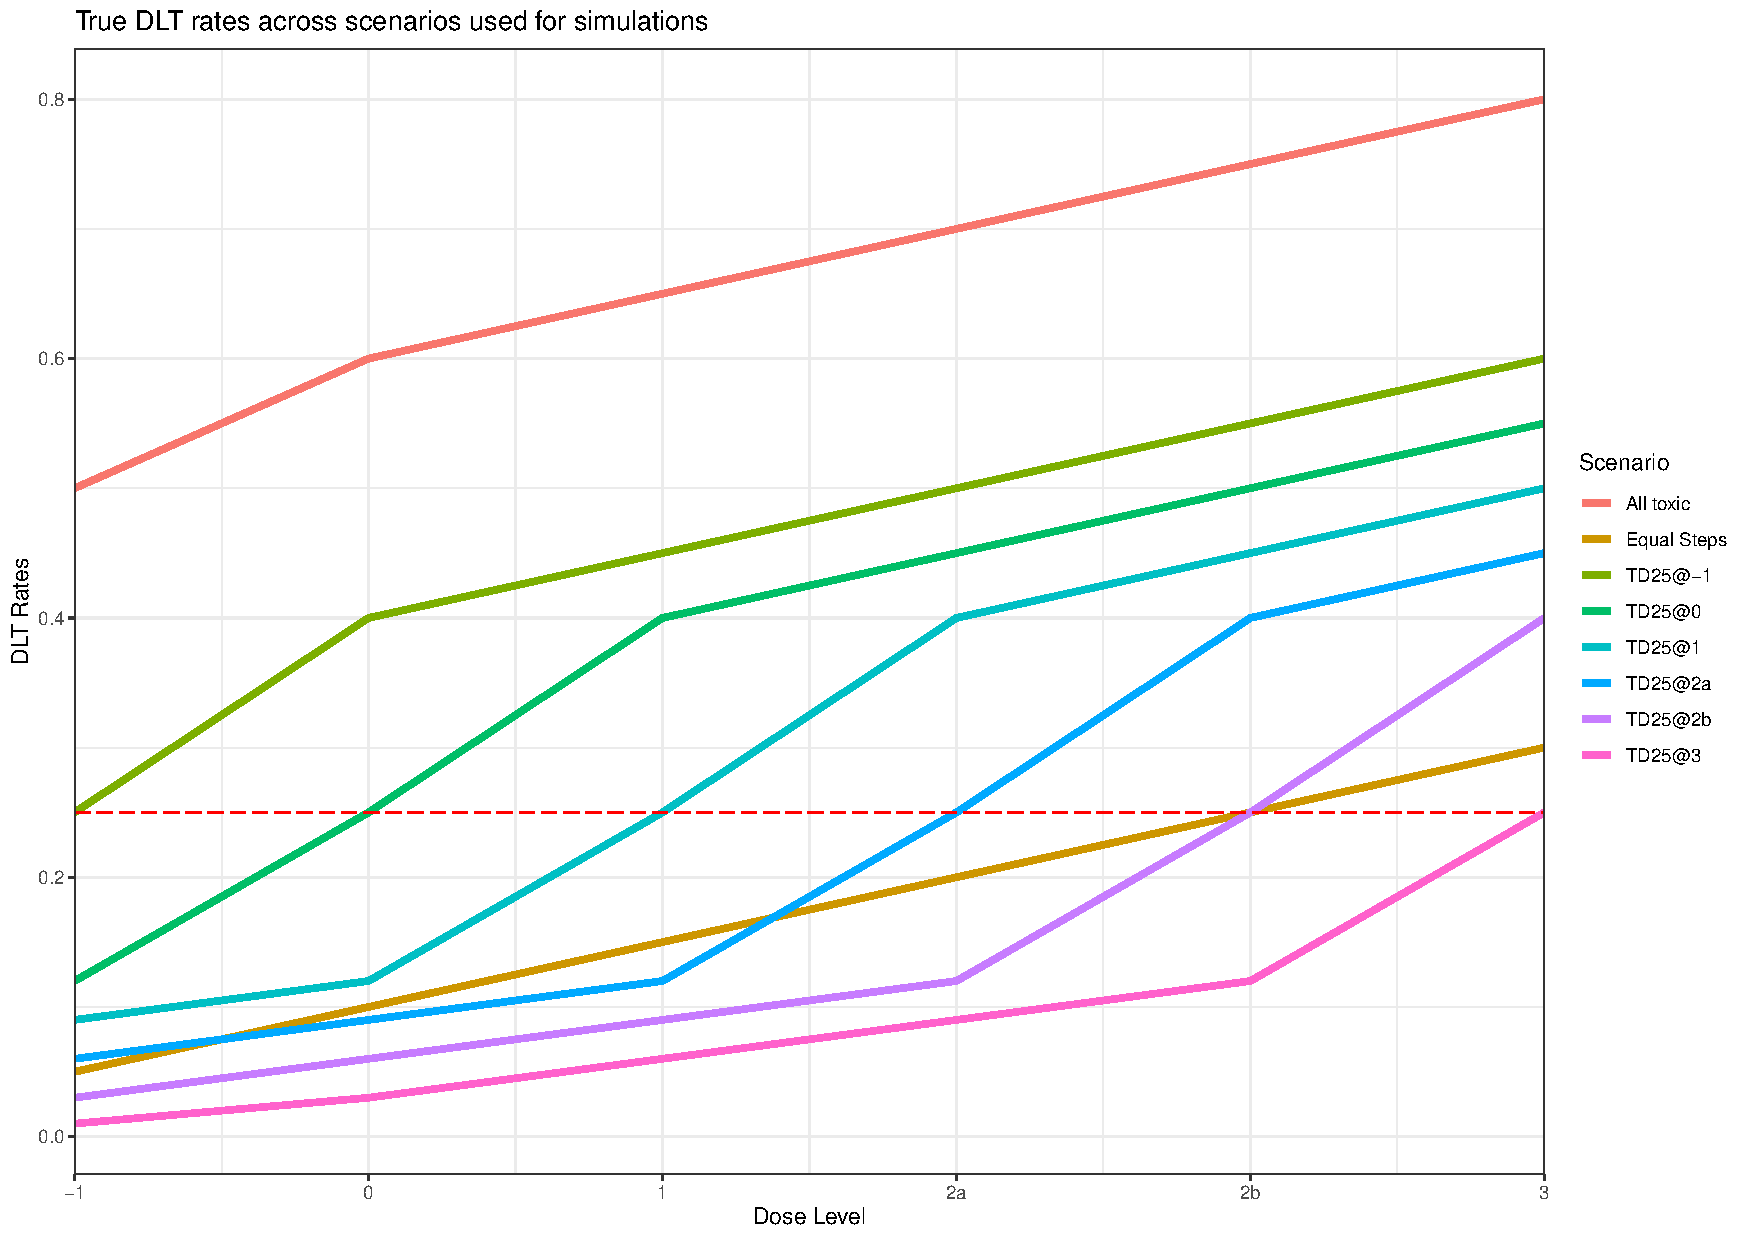
\includegraphics[width=\textwidth]{Adept-DLTRates}
\end{figure}
 
The original methodological papers by Wages et al. \cite{wagesUsingTimetoeventContinual2013,wagesContinualReassessmentMethod2011} only provide simulations for their examples using true DLT rates that are monotonically increasing which represented one of their possible orderings. We cannot tell how their design would perform under scenarios from different orderings. It is unclear as to why this wasn't examined. Initially, in ADePT-DDR we followed suit and only produced simulations under a monotonically increasing DLT rate (order where 2b is more toxic than 2a, Table \ref{tab_adept:OCorder1}). However, as we are unclear on the ordering of 2a and 2b there is a possibility that 2b is less toxic. So those initial simulations would not provide an accurate assessment of the design in that circumstance. This was the main motivation for running scenarios in Table \ref{tab_adept:OCorder2}, in which we see the design performs at a similar level regardless of the partial ordering. ADePT-DDR is a simple case of partial ordering as there are only two possible orderings and six dose-levels. For trials with higher numbers of orderings or dose-levels the number of scenarios that would have to be evaluated would increase which may be infeasible. Here it may be more beneficial to choose a handful of scenarios from multiple different orderings to cover a wider range of possible outcomes for the trial to assess the design. 

There are various features in this trial design that impact how it performs. The partial ordering caused by dose levels 2a and 2b adds complexity to design. If one of these dose-levels were to be removed or a normal ordering was assumed a standard TITE-CRM design could be used instead. However, this would take away from what the trial is trying to discover. This trial also has a long follow-up period due to potential late-onset toxicities and in turn, will have a long duration. The TITE component will allow for the duration to be a lot shorter than it would be otherwise. TITE-CRM designs allow for patients to be recruited sequentially and allocated a dose based on available information from patients already in the trial. The design for ADePT-DDR uses cohorts of three and a minimum follow-up period. The dose-escalation decisions will only be made every third patient after a specific amount of time. This is done for safety and practicality reasons but means that some patients may not be able to enter the trial and it also loses some of the benefits of the TITE-CRM. We also have a sample size of 60 patients but include a stopping rule for when a consensus is reached which means we often don't recruit the maximum sample size. Further simulations were produced to investigate how these features affected the trial. Tables \ref{tab_adept:Design_Comparison1} and \ref{tab_adept:Design_Comparison2} compares selection probabilities from the ADePT-DDR trial design with five alternative designs based on the two different orderings. Figures \ref{fig_adept:sims_order1} and \ref{fig_adept:sims_order2} visualise the result from each of these tables respectively. 10000 trials were simulated for each scenario which took 62 hours and 22 minutes to complete.  
 
\begin{enumerate}
	\item TITE-CRM design. This design assumes that partial ordering doesn't exist and that dose-level 2b is more toxic than 2a. A TITE-CRM is used instead of a PO-TITE-CRM. All other stopping rules and details remain the same. 
	\item PO (Partial Ordering design). This design removes the TITE component and uses a PO-CRM as detailed by \cite{wagesContinualReassessmentMethod2011}. This requires the removal of the minimum follow-up period so all dose allocation decisions are made once all 3 patients in a cohort have been observed for the full follow-up period of one year. All other stopping rules and details remain the same. 
	\item N = 30. This design uses a fixed sample size of 30 patients and removes the stopping rule for reaching consensus. The analysis is still conducted using the PO-TITE-CRM. All other stopping rules and details remain the same. 
	\item N = 60. This design uses a fixed sample size of 60 patients and removes the stopping rule for reaching consensus. The analysis is still conducted using the PO-TITE-CRM. All other stopping rules and details remain the same. 
	\item CS = 1. This design uses a cohort size (CS) of one. All other stopping rules remain the same.  
\end{enumerate} 

\begin{table} % Table for alterative designs scenarios 1-8
	
	\caption[Alternative designs selection probabilities for ordering 1.]{\label{tab_adept:Design_Comparison1}Selection probabilities of the TD25 and expected trial duration (in months) for the PO-TITE, TITE and PO-CRM designs as well as modified PO-TITE-CRM designs for scenarios 1-8 (where 2b is considered more toxic than 2a) based on 10000 simulated trials.}
	
	\centering
	\begin{singlespace}
		\resizebox{\linewidth}{!}{
			\fontsize{12}{11}\selectfont
			\begin{tabular}[t]{cccccccccccc}
			\toprule
			\multicolumn{3}{c}{ } & \multicolumn{6}{c}{Dose Levels} \\
			\cmidrule(l{3pt}r{3pt}){4-9}
			&  &  & -1 & 0 & 1 & 2a & 2b & 3 & Stop & Duration & Mean N\\
			\midrule
			Scenario & CRM details & Prior DLT & 0.01 & 0.04 & 0.08 & 0.16 & 0.25 & 0.35 &  &  & \\
			\cmidrule{1-12}
			\rowcolor{gray!6}   &  & True DLT rate & 0.25 & 0.4 & 0.45 & 0.5 & 0.55 & 0.6 &  &  & \\
			
			\rowcolor{gray!6}   & PO-TITE & P(select) & 0.68 & 0.18 & 0.05 & 0.01 & 0 & 0 & 0.08 & 57.61 & 26.38\\
			
			\rowcolor{gray!6}   & TITE & P(select) & 0.7 & 0.21 & 0.05 & 0.01 & 0 & 0 & 0.03 & 59.55 & 27.46\\
			
			\rowcolor{gray!6}   & PO & P(select) & 0.59 & 0.18 & 0.04 & 0.01 & 0 & 0 & 0.19 & 132.19 & 22.11\\
			
			\rowcolor{gray!6}   & N = 30 & P(select) & 0.67 & 0.19 & 0.05 & 0.01 & 0 & 0 & 0.08 & 60.02 & 27.72\\
			
			\rowcolor{gray!6}   & N = 60 & P(select) & 0.78 & 0.12 & 0.01 & 0 & 0 & 0 & 0.09 & 106.61 & 53.62\\
			
			\rowcolor{gray!6}  \multirow{-7}{*}{\centering\arraybackslash 1: TD25 @-1} & CS = 1 & P(select) & 0.63 & 0.17 & 0.04 & 0.01 & 0.01 & 0 & 0.15 & 87.62 & 22.44\\
			\cmidrule{1-12}
			&  & True DLT rate & 0.12 & 0.25 & 0.4 & 0.45 & 0.5 & 0.55 &  &  & \\
			
			& PO-TITE & P(select) & 0.23 & 0.51 & 0.2 & 0.03 & 0.02 & 0 & 0.01 & 64.06 & 29.97\\
			
			& TITE & P(select) & 0.22 & 0.54 & 0.2 & 0.04 & 0.01 & 0 &  & 63.5 & 29.65\\
			
			& PO & P(select) & 0.2 & 0.54 & 0.21 & 0.02 & 0.01 & 0 & 0.02 & 163.53 & 27.79\\
			
			& N = 30 & P(select) & 0.23 & 0.5 & 0.21 & 0.03 & 0.02 & 0 & 0.01 & 63.26 & 29.52\\
			
			& N = 60 & P(select) & 0.15 & 0.69 & 0.14 & 0.01 & 0 & 0 & 0.01 & 116.29 & 59\\
			
			\multirow{-7}{*}{\centering\arraybackslash 2: TD25 @0} & CS = 1 & P(select) & 0.25 & 0.46 & 0.19 & 0.03 & 0.02 & 0.01 & 0.04 & 105.41 & 27.59\\
			\cmidrule{1-12}
			\rowcolor{gray!6}   &  & True DLT rate & 0.09 & 0.12 & 0.25 & 0.4 & 0.45 & 0.5 &  &  & \\
			
			\rowcolor{gray!6}   & PO-TITE & P(select) & 0.02 & 0.2 & 0.55 & 0.14 & 0.09 & 0.01 &  & 67.74 & 32.01\\
			
			\rowcolor{gray!6}   & TITE & P(select) & 0.01 & 0.2 & 0.54 & 0.2 & 0.04 & 0 &  & 64.44 & 30.18\\
			
			\rowcolor{gray!6}   & PO & P(select) & 0.02 & 0.16 & 0.59 & 0.14 & 0.07 & 0.01 &  & 178.12 & 30.43\\
			
			\rowcolor{gray!6}   & N = 30 & P(select) & 0.01 & 0.19 & 0.52 & 0.15 & 0.12 & 0.01 &  & 64.04 & 29.96\\
			
			\rowcolor{gray!6}   & N = 60 & P(select) & 0 & 0.14 & 0.7 & 0.1 & 0.06 & 0 &  & 117.89 & 59.89\\
			
			\rowcolor{gray!6}  \multirow{-7}{*}{\centering\arraybackslash 3: TD25 @1} & CS = 1 & P(select) & 0.05 & 0.18 & 0.51 & 0.14 & 0.09 & 0.02 & 0.01 & 114.18 & 30.13\\
			\cmidrule{1-12}
			&  & True DLT rate & 0.06 & 0.09 & 0.12 & 0.25 & 0.4 & 0.45 &  &  & \\
			
			& PO-TITE & P(select) & 0 & 0.02 & 0.22 & 0.48 & 0.23 & 0.05 &  & 69.91 & 33.22\\
			
			& TITE & P(select) & 0 & 0.02 & 0.21 & 0.56 & 0.18 & 0.03 &  & 66.99 & 31.59\\
			
			& PO & P(select) & 0 & 0.02 & 0.22 & 0.49 & 0.22 & 0.05 &  & 189.69 & 32.52\\
			
			& N = 30 & P(select) & 0 & 0.01 & 0.22 & 0.45 & 0.27 & 0.05 &  & 64.1 & 29.99\\
			
			& N = 60 & P(select) & 0 & 0 & 0.18 & 0.64 & 0.18 & 0.01 &  & 118.01 & 59.96\\
			
			\multirow{-7}{*}{\centering\arraybackslash 4: TD25 @2a} & CS = 1 & P(select) & 0.03 & 0.02 & 0.22 & 0.45 & 0.2 & 0.08 &  & 113.77 & 30.01\\
			\cmidrule{1-12}
			\rowcolor{gray!6}   &  & True DLT rate & 0.03 & 0.06 & 0.09 & 0.12 & 0.25 & 0.4 &  &  & \\
			
			\rowcolor{gray!6}   & PO-TITE & P(select) & 0 & 0 & 0.02 & 0.3 & 0.43 & 0.25 &  & 70.6 & 33.6\\
			
			\rowcolor{gray!6}   & TITE & P(select) & 0 & 0 & 0.02 & 0.22 & 0.56 & 0.19 &  & 68.34 & 32.34\\
			
			\rowcolor{gray!6}   & PO & P(select) & 0 & 0 & 0.03 & 0.26 & 0.44 & 0.27 &  & 194.41 & 33.38\\
			
			\rowcolor{gray!6}   & N = 30 & P(select) & 0 & 0 & 0.03 & 0.3 & 0.43 & 0.24 &  & 64.11 & 29.99\\
			
			\rowcolor{gray!6}   & N = 60 & P(select) & 0 & 0 & 0 & 0.24 & 0.61 & 0.14 &  & 118.08 & 59.99\\
			
			\rowcolor{gray!6}  \multirow{-7}{*}{\centering\arraybackslash 5: TD25 @2b} & CS = 1 & P(select) & 0.01 & 0 & 0.02 & 0.26 & 0.4 & 0.3 &  & 110.26 & 29\\
			\cmidrule{1-12}
			&  & True DLT rate & 0.01 & 0.03 & 0.06 & 0.09 & 0.12 & 0.25 &  &  & \\
			
			& PO-TITE & P(select) & 0 & 0 & 0 & 0.09 & 0.13 & 0.78 &  & 65.78 & 30.92\\
			
			& TITE & P(select) & 0 & 0 & 0 & 0.03 & 0.23 & 0.73 &  & 65.6 & 30.82\\
			
			& PO & P(select) & 0 & 0 & 0 & 0.08 & 0.12 & 0.8 &  & 183.48 & 31.4\\
			
			& N = 30 & P(select) & 0 & 0 & 0 & 0.1 & 0.14 & 0.75 &  & 64.12 & 30\\
			
			& N = 60 & P(select) & 0 & 0 & 0 & 0.06 & 0.1 & 0.85 &  & 118.09 & 60\\
			
			\multirow{-7}{*}{\centering\arraybackslash 6: TD25 @3} & CS = 1 & P(select) & 0.01 & 0 & 0 & 0.06 & 0.1 & 0.83 &  & 92.92 & 23.98\\
			\cmidrule{1-12}
			\rowcolor{gray!6}   &  & True DLT rate & 0.05 & 0.1 & 0.15 & 0.2 & 0.25 & 0.3 &  &  & \\
			
			\rowcolor{gray!6}   & PO-TITE & P(select) & 0 & 0.03 & 0.12 & 0.31 & 0.28 & 0.26 &  & 67.25 & 31.74\\
			
			\rowcolor{gray!6}   & TITE & P(select) & 0 & 0.03 & 0.14 & 0.3 & 0.32 & 0.21 &  & 65.22 & 30.61\\
			
			\rowcolor{gray!6}   & PO & P(select) & 0.01 & 0.03 & 0.14 & 0.3 & 0.27 & 0.25 &  & 186.6 & 31.96\\
			
			\rowcolor{gray!6}   & N = 30 & P(select) & 0 & 0.02 & 0.12 & 0.3 & 0.3 & 0.25 &  & 64.07 & 29.97\\
			
			\rowcolor{gray!6}   & N = 60 & P(select) & 0 & 0 & 0.07 & 0.33 & 0.35 & 0.25 &  & 118.04 & 59.97\\
			
			\rowcolor{gray!6}  \multirow{-7}{*}{\centering\arraybackslash 7: Equal steps} & CS = 1 & P(select) & 0.03 & 0.02 & 0.09 & 0.24 & 0.23 & 0.39 &  & 101.81 & 26.55\\
			\cmidrule{1-12}
			&  & True DLT rate & 0.5 & 0.6 & 0.65 & 0.7 & 0.75 & 0.8 &  &  & \\
			
			& PO-TITE & P(select) & 0.26 & 0 & 0 & 0 & 0 & 0 & 0.74 & 39.19 & 16.14\\
			
			& TITE & P(select) & 0.37 & 0 & 0 & 0 & 0 & 0 & 0.63 & 44.65 & 19.17\\
			
			& PO & P(select) & 0.13 & 0 & 0 & 0 & 0 & 0 & 0.86 & 70.38 & 10.92\\
			
			& N = 30 & P(select) & 0.23 & 0 & 0 & 0 & 0 & 0 & 0.77 & 41.35 & 17.34\\
			
			& N = 60 & P(select) & 0.13 & 0 & 0 & 0 & 0 & 0 & 0.87 & 47.35 & 20.68\\
			
			\multirow{-7}{*}{\centering\arraybackslash 8: All toxic} & CS = 1 & P(select) & 0.33 & 0 & 0 & 0 & 0 & 0 & 0.67 & 46.43 & 10.51\\
			\bottomrule
		\end{tabular}}
	\end{singlespace}
\end{table}

\begin{table} % Table for alterative designs scenarios 9-16
	
	\caption[Alternative designs selection probabilities for ordering 2.]{\label{tab_adept:Design_Comparison2}Selection probabilities of the TD25 and expected trial duration (in months) for the PO-TITE, TITE and PO-CRM designs as well as modified PO-TITE-CRM designs for scenarios 9-16 (where 2a is considered more toxic than 2b) based on 10000 simulated trials.}
	
	\centering
	\begin{singlespace}
		\resizebox{\linewidth}{!}{
			\fontsize{12}{11}\selectfont
			\begin{tabular}[t]{cccccccccccc}
			\toprule
			\multicolumn{3}{c}{ } & \multicolumn{6}{c}{Dose Levels} \\
			\cmidrule(l{3pt}r{3pt}){4-9}
			&  &  & -1 & 0 & 1 & 2a & 2b & 3 & Stop & Duration & Mean N\\
			\midrule
			Scenario & CRM details & Prior DLT & 0.01 & 0.04 & 0.08 & 0.16 & 0.25 & 0.35 &  &  & \\
			\cmidrule{1-12}
			\rowcolor{gray!6}   &  & True DLT rate & 0.25 & 0.4 & 0.45 & 0.55 & 0.5 & 0.6 &  &  & \\
			
			\rowcolor{gray!6}   & PO-TITE & P(select) & 0.67 & 0.19 & 0.05 & 0 & 0.01 & 0 & 0.08 & 57.35 & 26.23\\
			
			\rowcolor{gray!6}   & TITE & P(select) & 0.7 & 0.21 & 0.05 & 0 & 0 & 0 & 0.03 & 59.34 & 27.34\\
			
			\rowcolor{gray!6}   & PO & P(select) & 0.58 & 0.17 & 0.04 & 0 & 0 & 0 & 0.2 & 131.46 & 21.98\\
			
			\rowcolor{gray!6}   & N = 30 & P(select) & 0.68 & 0.18 & 0.04 & 0 & 0.01 & 0 & 0.09 & 59.85 & 27.62\\
			
			\rowcolor{gray!6}   & N = 60 & P(select) & 0.78 & 0.13 & 0.01 & 0 & 0 & 0 & 0.09 & 106.5 & 53.56\\
			
			\rowcolor{gray!6}  \multirow{-7}{*}{\centering\arraybackslash 9: TD25 @-1} & CS = 1 & P(select) & 0.62 & 0.16 & 0.05 & 0 & 0.01 & 0 & 0.15 & 87.6 & 22.43\\
			\cmidrule{1-12}
			&  & True DLT rate & 0.12 & 0.25 & 0.4 & 0.5 & 0.45 & 0.55 &  &  & \\
			
			& PO-TITE & P(select) & 0.23 & 0.52 & 0.2 & 0.02 & 0.02 & 0 & 0.01 & 64.02 & 29.95\\
			
			& TITE & P(select) & 0.21 & 0.56 & 0.19 & 0.02 & 0.01 & 0 &  & 63.57 & 29.69\\
			
			& PO & P(select) & 0.2 & 0.54 & 0.2 & 0.01 & 0.02 & 0 & 0.02 & 163.06 & 27.7\\
			
			& N = 30 & P(select) & 0.24 & 0.51 & 0.2 & 0.02 & 0.03 & 0 & 0.01 & 63.35 & 29.57\\
			
			& N = 60 & P(select) & 0.15 & 0.7 & 0.13 & 0 & 0.01 & 0 & 0.01 & 116.22 & 58.96\\
			
			\multirow{-7}{*}{\centering\arraybackslash 10: TD25 @0} & CS = 1 & P(select) & 0.25 & 0.47 & 0.19 & 0.02 & 0.03 & 0.01 & 0.04 & 105.04 & 27.49\\
			\cmidrule{1-12}
			\rowcolor{gray!6}   &  & True DLT rate & 0.09 & 0.12 & 0.25 & 0.45 & 0.4 & 0.5 &  &  & \\
			
			\rowcolor{gray!6}   & PO-TITE & P(select) & 0.02 & 0.2 & 0.55 & 0.09 & 0.14 & 0.01 &  & 68 & 32.15\\
			
			\rowcolor{gray!6}   & TITE & P(select) & 0.01 & 0.22 & 0.58 & 0.14 & 0.04 & 0 &  & 64.86 & 30.41\\
			
			\rowcolor{gray!6}   & PO & P(select) & 0.03 & 0.17 & 0.59 & 0.09 & 0.12 & 0.01 &  & 177.68 & 30.35\\
			
			\rowcolor{gray!6}   & N = 30 & P(select) & 0.02 & 0.2 & 0.51 & 0.1 & 0.16 & 0.01 &  & 64.03 & 29.95\\
			
			\rowcolor{gray!6}   & N = 60 & P(select) & 0 & 0.14 & 0.71 & 0.05 & 0.1 & 0 &  & 117.88 & 59.88\\
			
			\rowcolor{gray!6}  \multirow{-7}{*}{\centering\arraybackslash 11: TD25 @1} & CS = 1 & P(select) & 0.05 & 0.17 & 0.53 & 0.09 & 0.13 & 0.02 & 0.01 & 113.98 & 30.07\\
			\cmidrule{1-12}
			&  & True DLT rate & 0.06 & 0.09 & 0.12 & 0.25 & 0.15 & 0.45 &  &  & \\
			
			& PO-TITE & P(select) & 0 & 0.01 & 0.08 & 0.44 & 0.33 & 0.14 &  & 70.52 & 33.56\\
			
			& TITE & P(select) & 0 & 0.02 & 0.14 & 0.26 & 0.45 & 0.14 &  & 67.23 & 31.73\\
			
			& PO & P(select) & 0.01 & 0.02 & 0.09 & 0.45 & 0.28 & 0.15 &  & 194.42 & 33.38\\
			
			& N = 30 & P(select) & 0 & 0.01 & 0.08 & 0.42 & 0.35 & 0.14 &  & 64.09 & 29.98\\
			
			& N = 60 & P(select) & 0 & 0 & 0.03 & 0.57 & 0.33 & 0.07 &  & 117.98 & 59.94\\
			
			\multirow{-7}{*}{\centering\arraybackslash 12: TD25 @2a} & CS = 1 & P(select) & 0.02 & 0.01 & 0.07 & 0.4 & 0.32 & 0.18 &  & 113.02 & 29.8\\
			\cmidrule{1-12}
			\rowcolor{gray!6}   &  & True DLT rate & 0.03 & 0.06 & 0.09 & 0.35 & 0.25 & 0.4 &  &  & \\
			
			\rowcolor{gray!6}   & PO-TITE & P(select) & 0 & 0 & 0.15 & 0.31 & 0.43 & 0.11 &  & 69.8 & 33.16\\
			
			\rowcolor{gray!6}   & TITE & P(select) & 0 & 0.01 & 0.26 & 0.36 & 0.28 & 0.1 &  & 65.95 & 31.02\\
			
			\rowcolor{gray!6}   & PO & P(select) & 0 & 0.01 & 0.14 & 0.34 & 0.43 & 0.1 &  & 190.68 & 32.7\\
			
			\rowcolor{gray!6}   & N = 30 & P(select) & 0 & 0 & 0.15 & 0.3 & 0.44 & 0.11 &  & 64.12 & 30\\
			
			\rowcolor{gray!6}   & N = 60 & P(select) & 0 & 0 & 0.1 & 0.29 & 0.57 & 0.04 &  & 118.07 & 59.99\\
			
			\rowcolor{gray!6}  \multirow{-7}{*}{\centering\arraybackslash 13: TD25 @2b} & CS = 1 & P(select) & 0.02 & 0 & 0.14 & 0.27 & 0.4 & 0.17 &  & 112.27 & 29.58\\
			\cmidrule{1-12}
			&  & True DLT rate & 0.01 & 0.03 & 0.06 & 0.12 & 0.09 & 0.25 &  &  & \\
			
			& PO-TITE & P(select) & 0 & 0 & 0 & 0.13 & 0.09 & 0.78 &  & 65.58 & 30.81\\
			
			& TITE & P(select) & 0 & 0 & 0 & 0.04 & 0.21 & 0.74 &  & 65.66 & 30.86\\
			
			& PO & P(select) & 0 & 0 & 0 & 0.13 & 0.07 & 0.8 &  & 183.9 & 31.47\\
			
			& N = 30 & P(select) & 0 & 0 & 0 & 0.13 & 0.11 & 0.75 &  & 64.12 & 30\\
			
			& N = 60 & P(select) & 0 & 0 & 0 & 0.09 & 0.06 & 0.85 &  & 118.09 & 60\\
			
			\multirow{-7}{*}{\centering\arraybackslash 14: TD25 @3} & CS = 1 & P(select) & 0.01 & 0 & 0 & 0.1 & 0.07 & 0.82 &  & 93.1 & 24.03\\
			\cmidrule{1-12}
			\rowcolor{gray!6}   &  & True DLT rate & 0.05 & 0.1 & 0.15 & 0.25 & 0.2 & 0.3 &  &  & \\
			
			\rowcolor{gray!6}   & PO-TITE & P(select) & 0 & 0.02 & 0.12 & 0.32 & 0.27 & 0.26 &  & 67.17 & 31.69\\
			
			\rowcolor{gray!6}   & TITE & P(select) & 0 & 0.03 & 0.19 & 0.27 & 0.28 & 0.24 &  & 65.01 & 30.49\\
			
			\rowcolor{gray!6}   & PO & P(select) & 0 & 0.03 & 0.16 & 0.32 & 0.26 & 0.23 &  & 186.35 & 31.92\\
			
			\rowcolor{gray!6}   & N = 30 & P(select) & 0 & 0.02 & 0.13 & 0.3 & 0.29 & 0.25 &  & 64.1 & 29.99\\
			
			\rowcolor{gray!6}   & N = 60 & P(select) & 0 & 0 & 0.07 & 0.36 & 0.31 & 0.25 &  & 117.97 & 59.94\\
			
			\rowcolor{gray!6}  \multirow{-7}{*}{\centering\arraybackslash 15: Equal steps} & CS = 1 & P(select) & 0.03 & 0.02 & 0.09 & 0.23 & 0.23 & 0.4 &  & 102.22 & 26.67\\
			\cmidrule{1-12}
			&  & True DLT rate & 0.5 & 0.6 & 0.65 & 0.75 & 0.7 & 0.8 &  &  & \\
			
			& PO-TITE & P(select) & 0.27 & 0 & 0 & 0 & 0 & 0 & 0.73 & 39.14 & 16.11\\
			
			& TITE & P(select) & 0.37 & 0 & 0 & 0 & 0 & 0 & 0.63 & 44.23 & 18.94\\
			
			& PO & P(select) & 0.13 & 0 & 0 & 0 & 0 & 0 & 0.87 & 69.79 & 10.81\\
			
			& N = 30 & P(select) & 0.23 & 0 & 0 & 0 & 0 & 0 & 0.77 & 41.18 & 17.24\\
			
			& N = 60 & P(select) & 0.13 & 0 & 0 & 0 & 0 & 0 & 0.87 & 47.29 & 20.64\\
			
			\multirow{-7}{*}{\centering\arraybackslash 16: All toxic} & CS = 1 & P(select) & 0.33 & 0 & 0 & 0 & 0 & 0 & 0.67 & 45.76 & 10.31\\
			\bottomrule
	\end{tabular}}
\end{singlespace}
\end{table}

\begin{figure}[h!]
	\centering
	\caption[Plot of simulations comparing designs for ordering 1.]{Plot of the simulation results presented in Table \ref{tab_adept:Design_Comparison1} detailing selection probabilities for multiple designs across scenarios 1-8 (where 2b is considered more toxic than 2a).}
	\label{fig_adept:sims_order1}
	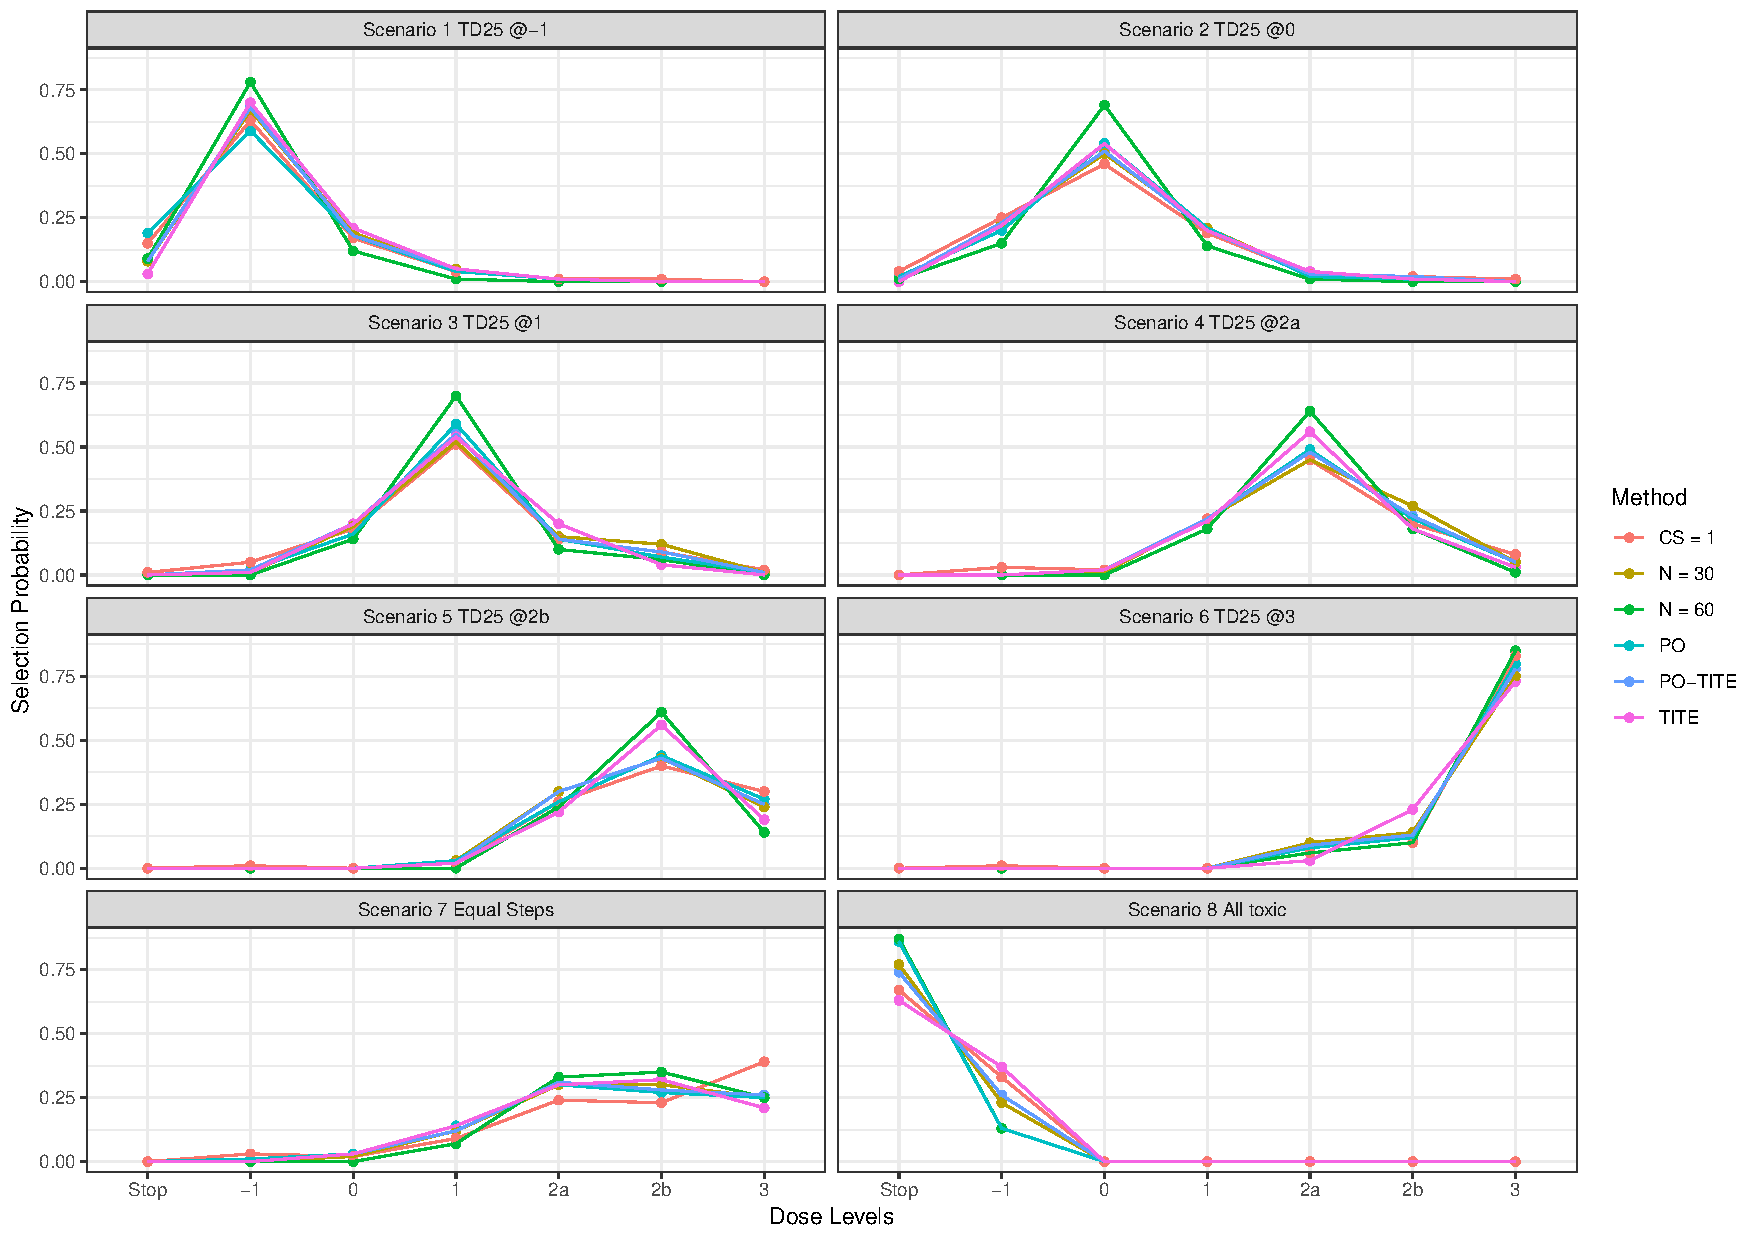
\includegraphics[width=\textwidth]{Adept-SimsOrder1}
\end{figure}

\begin{figure}[h!]
	\centering
	\caption[Plot of simulations comparing designs for ordering 2.]{Plot of the simulation results presented in Table \ref{tab_adept:Design_Comparison2} detailing selection probabilities for multiple designs across scenarios 9-16 (where 2a is considered more toxic than 2b).}
	\label{fig_adept:sims_order2}
	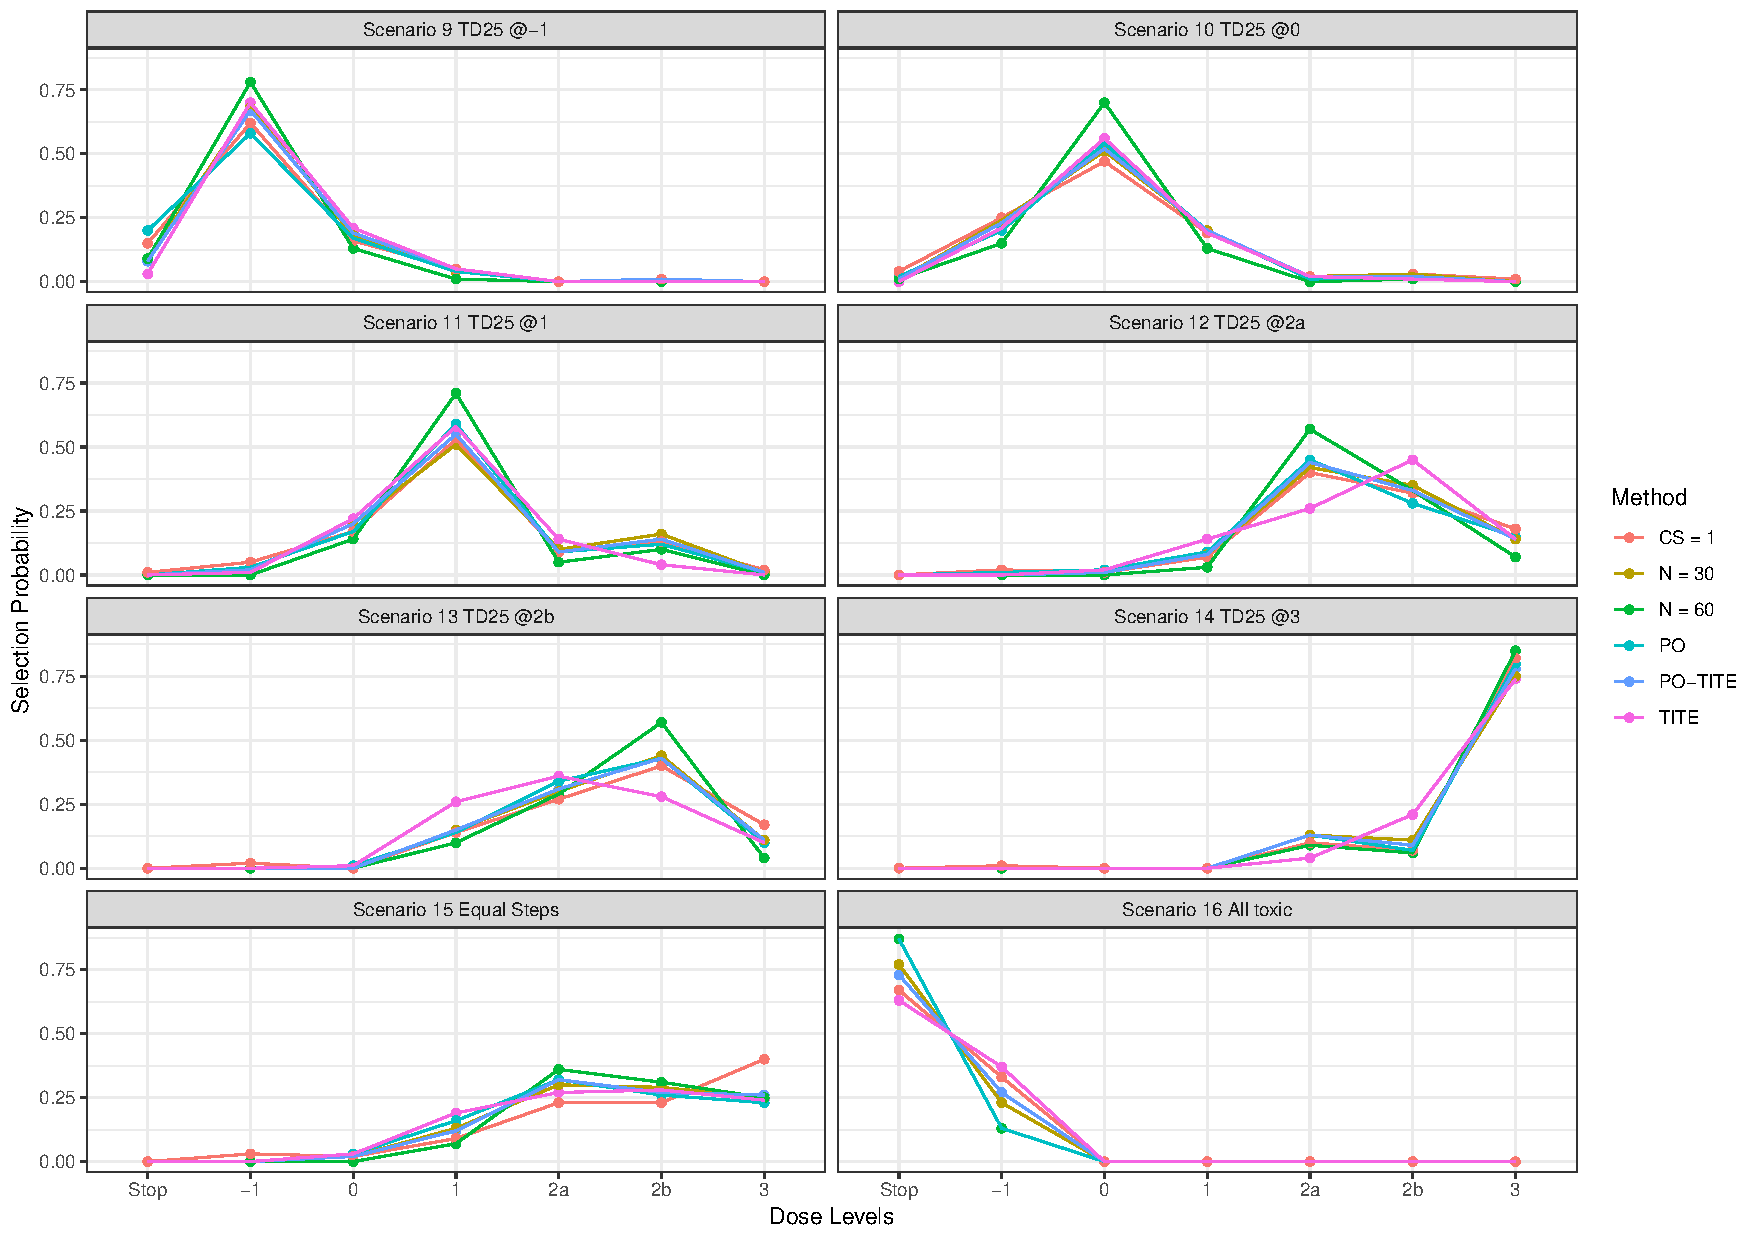
\includegraphics[width=\textwidth]{Adept-SimsOrder2}
\end{figure}

The TITE-CRM performs similarly to our original design for scenarios 1-8 where 2a is assumed less toxic than 2b (Table \ref{tab_adept:OCorder1}). Compared to the PO-TITE design we see increases in probability selection for scenarios 4 and 5 where the target dose is at 2a and 2b respectively. This increase in performance can be attributed to the fact that the partial ordering no longer exists as we have assumed an ordering. The lower selection probabilities for the PO-TITE-CRM can be seen as the price to pay for the uncertainty of not knowing the order of 2a and 2b. However, the TITE-CRM underperforms in scenarios 9-16 where 2a is assumed more toxic than 2b. Specifically, scenarios 12 and 13 where it fails to identify the TD25 the majority of the time. 

The PO-CRM design without a TITE component also performs similarly except for scenarios 1, 8, 9 and 16 where the trial stops more regularly for excess toxicity at the lowest dose. This would be because patients complete the full follow-up window before the next dose allocation decision is made. In a TITE setting a new cohort could be recruited before patients in previous cohorts experience a DLT. The main difference between these designs is the trial duration. Without the TITE component the trial duration is significantly longer, with the average length ranging from 70 to 195 months compared to 39 to 71 months for PO-TITE-CRM. 

The design with a fixed sample size of 30 performs is comparable to our design with the sample size of 60 and the consensus stopping rule. With a sample size of 30 selection probabilities are only 2-5\% lower. For the design with 60 patients, we see much improved operating characteristics with selection probabilities ranging from 31\% to 85\% for the various scenarios. Even though our original design specifies a sample size of 60 we rarely ever reach it as we often stop for consensus hence why this design performs better. The trade-off here is trial duration. Recruitment and follow-up under the constraints of these simulations will take much longer compared to our specification which is not ideal for an early-phase trial. Originally our design had a fixed sample size of 30 but as the clinicians wanted a dose expansion cohort we opted to use the consensus rule to ensure a minimum number of patients would be treated at the TD25. 

For the design with no cohorts, or cohort size of one, we see somewhat comparable performance to that of the PO-TITE-CRM design. The design performs similarly for scenarios where the TD25 is at the lowest or highest dose level but underperforms for the more complex scenarios in terms of selection probabilities. This discrepancy in performance may be related to how the simulations recruit patients into the trial and the large DLT follow-up period. Meaning more frequent dose allocation decisions are being made each with less available information. This also leads to the no cohorts design having a longer duration. Patients entered into the trial in cohorts of three won't having to wait the full minimum follow-up period between patients within the cohort.



%----------------------------------------------------------------------------------------
%	SECTION 5
%-------------------------.

\section{Discussion}  
\label{adept:Discussion}

The PO-CRM and PO-TITE-CRM designs offer solutions to the issue of partial ordering where the order of the treatments is only partially known. The original methodology details that this issue commonly arises in trials of multiple agents, where each drug individually may follow the monotonicity assumption but when combined at certain dose levels this may not hold. This issue is typically dealt with by fixing the dose of one of the agents and escalating in the other or escalating in both agents simultaneously. This means certain drug combinations that are clinically relevant may not be investigated or even considered.  
 
Here we have shown that these issues can also arise in other situations. Even though the ADePT-DDR trial uses multiple agents the issue of partial ordering still occurs due to the varying treatment dose and schedule for one of its agents AZD6738. Implementing the PO-TITE-CRM design allowed us to deal with this issue effectively. There may be other factors or variables in single-agent dose-finding trials that would lead to the issue of partial ordering and would warrant the use of either PO-CRM or PO-TITE-CRM. The small literature review conducted highlighted this may be the first instance of the PO-TITE-CRM design being applied. It is important to note that although this methodology takes into account all the various orderings the main aim is to identify the TD and does not attempt to identify the order that is more correct. 

Compared to other CRM based designs only a few additional pieces of information are required to implement the PO-CRM design. More importantly is the number of toxicity orderings and prior probabilities for the orders. Dependent on how many dose combinations are available it may not be feasible to investigate all combinations and all orderings. Careful thought and consideration should be given to the combinations and orderings selected which would require input from all relevant investigators. In terms of priors for orderings if no prior information is available all orders should be treated as equally likely to occur. Extending this design to the PO-TITE-CRM requires a fit for purpose weight function and is applied similarly to the TITE-CRM methodology. There is an R package available with functions that can be used to run and simulate a PO-CRM trial. These functions were extended to included weighted dose toxicity models as described in this chapter to implement PO-TITE-CRM into ADePT-DDR. The lack of available software for PO-TITE-CRM specifically may be one of the reasons for its lack of use.

In terms of ADePT-DDR, dose combinations were decided upon by the clinical investigators. The issue of partial ordering was due to the dose-levels 2a and 2b as such this methodology was employed to deal with that scenario. Meaning that this is a very simple example of partial ordering as we only have two possible orderings and six dose levels. The necessity of implementing this methodology was discussed and whether or not adopting an easier solution by simply altering the dose levels would have been better. Ultimately, the dose levels selected by the clinicians were deemed the most relevant with the TD25 likely to be one of these doses.     
 
Simulations and operating characteristics were the main tools used to assess the designs performance as well as help understand the impact of sample size and stopping rules. This was an iterative process that involved running multiple iterations of simulations under various scenarios until the design was finalised. A key point is that scenarios from simulations should account for each of the possible orderings. ADePT-DDR only has two orderings, we ran scenarios for both. For a trial with a greater number of orderings, this may be unfeasible but at least some scenarios should be assessed to ensure the design is behaving as expected. Overall, the design operating characteristics performed reasonably well even in difficult scenarios. 

One limitation of the simulations is how the time-to-event data is generated. The time of DLTs is sampled from a uniform distribution $U(0, 413)$, where the time of the DLT can occur at any time between the patient beginning treatment and the end of follow-up (413 days). Using this uniform distribution implies that a DLT has an equal probability of occurring at any time-point in the observation window. This may not be an accurate representation of what happens in the actual trial. Similar comments can be made about the accrual rate used in the simulations. Here we specified the recruitment of one patient per month which is in no way guaranteed for the actual trial. Wages et al. \cite{wagesUsingTimetoeventContinual2013}, when presenting this methodology investigated four different applications of the PO-TITE-CRM which used different models to enroll patients and allocate DLTs. Results across these four applications were comparable. 

The simulations are also able to instantaneously determine dose-levels for incoming cohorts with all available information. This does not fully reflect the process in which dose-escalation decisions would be made during the actual running of the trial. The analysis would require a data snapshot and time would have to be spent cleaning the data and determining the next dose-level. Meaning any data from the point of the snapshot would not be included in any dose escalation/de-escalation decisions. 

Similarly, there may also be limitations with some of the design choices made concerning to cohort size and sample size. These were investigated alongside a variety of other trial designs that could have been implemented. This was done to validate the choices we made with the design and highlight the differences in operating characteristics due to the varying assumptions and components in the designs. The standard PO-CRM had a much longer average duration due to the lack of TITE component whereas a standard TITE-CRM overall performs better but assumes the ordering of toxicity is known. 


%----------------------------------------------------------------------------------------
%	SECTION 6
%-------------------------.

\section{Conclusion}  
\label{adept:Conclusion}

The monotonicity assumption may not hold in some dose-finding trials leading to the issue of partial ordering. This could be due to multiple-agents being investigated or varying factors in single-agent treatment. PO-CRM and PO-TITE-CRM are important trial designs as they address this core issue. ADePT-DDR is a platform trial with its initial component being a dose-finding trial investigating AZD6738 in combination with radiotherapy, of which the toxicity ordering for two of the dose levels for investigation is unknown. The PO-TITE-CRM design allows for us to deal with this issue of partial ordering as well as account for potential late-onset toxicities due to radiotherapy with its TITE component. 

We detail the issue of partial ordering and how we implemented the trial design, in what we believe is the first real-world application of this design. A large amount of simulation work is required to assess the performance of the design. This is often an iterative process to refine decisions that were made and often requires input from both clinical and statistical investigators. We recommend running several varied scenarios for each potential ordering that will be investigated. Finally, we also compared the implementation of PO-TITE-CRM to various other designs. 

 
% Chapter Template

\chapter{Extensions to the Wages and Tait trial design} % Main chapter title

\label{WT} % For referencing this chapter elsewhere, use \ref{WT}

%----------------------------------------------------------------------------------------
%	SECTION 1
%----------------------------------------------------------------------------------------

\section{Introduction}
\label{WT:Introduction}

Typically the main aim of Phase \RN{1} clinical trials is to identify the maximum tolerated dose (MTD) of the treatment being investigated. The MTD is usually determined under the cytotoxic assumption which assumes the most toxic dose is the most efficacious. With model-based designs such as the continual reassessment method (CRM) \cite{oquigleyContinualReassessmentMethod1990} escalation occurs to identify the dose with an associated probability of toxicity based on a pre-defined target. Dose selection and escalation decisions do not consider efficacy rather they are determined based on the occurrence of toxicities. The cytotoxic assumption here implies that the rate of efficacy increases monotonically with the dose-level and probability of toxicity. Subsequent Phase \RN{2} trials aim to assess the efficacy of the treatment at the recommended dose (MTD). Usually, these two phases are conducted independently of each other and as such, the ability to share information across the phases is somewhat lost. 

For treatments like chemotherapy which kills all cells including cancer cells \cite{corrieCytotoxicChemotherapyClinical2008}, the cytotoxic assumption is valid. However, the emergence of modern treatments such as immunotherapy and molecular targeted agents challenges this paradigm. Immunotherapy is a form of treatment that utilises the body's immune system to fight cancer \cite{mellmanCancerImmunotherapyComes2011}. Molecular targeted agents (MTA) work by interfering with specific molecules responsible for the growth, spread, and progression of cancer \cite{soriaAddedValueMolecular2011}. The monotonic assumption of dose-efficacy may not hold for these new types of treatments. Furthermore, these treatments, in general, are less toxic than traditional cytotoxic agents such as chemotherapy therefore it is possible the most efficacious dose may occur at a dose-level below the MTD \cite{ahnOptimalBiologicalDose2016}. This produces some methodological challenges for dose-finding trials. Instead of trying to identify the MTD, the goal would be to determine the optimal biological dose (OBD). Depending on the aims of the trial and the design implemented the definition of the OBD may vary. The OBD could be a dose that provides the maximum probability of efficacy with the probability of toxicity being less than a pre-defined target value, or the dose that has a beneficial trade-off between toxicity and efficacy. To determine an optimal dose both toxicity and efficacy outcomes need to be considered and this leads to a need for joint phase \RN{1}/\RN{2} trial designs. Here we will briefly explore some of these designs. 

Braun \cite{braunBivariateContinualReassessment2002} proposed the bivariate continual reassessment method (bCRM), an extension to the CRM which incorporates competing outcomes for both toxicity and disease progression. The design models the probabilities of toxicity and progression independently, it is suggested that either empiric, logistic, or hyperbolic tangent functions are used dependent on their biological plausibility. Both outcomes are then combined into a joint distribution which is used to estimate posterior means based on priors and observed data. 

Thall \& Cook \cite{thallDosefindingBasedEfficacytoxicity2004} developed EffTox, a Bayesian adaptive dose-finding trial based on trade-offs between the probabilities of toxicity and efficacy. Marginal probabilities of efficacy and toxicity at each dose are modelled and used with utility contours to determine the desirability of each dose based on posterior probabilities of efficacy and toxicity \cite{brockImplementingEffToxDosefinding2017}. 

Zhou et al. \cite{zhouUtilitybasedBayesianOptimal2019} introduced a Utility-based Bayesian Optimal Interval (U-BOIN) phase \RN{1}/\RN{2} design to identify the OBD. This design is an extension of the Bayesian optimal interval (BOIN) design for phase \RN{1} trials developed by Liu and Yuan \cite{liuBAYESIANDATAAUGMENTATION2013}. U-BOIN jointly models toxicity and efficacy with a multinomial-Dirichlet model and uses a utility function to measure the dose risk-benefit trade-off. The design consists of two seamless stages. Firstly, in stage \RN{1} the BOIN design is used to explore the dose levels and determine a set of admissible doses and collect preliminary efficacy data. In stage \RN{2} posterior estimates of utility for each dose are continuously updated after each cohort using toxicity and efficacy data from both stages. 

Zhang et al. \cite{zhangAdaptiveDosefindingDesign2006} introduced the trivariate CRM (TriCRM) design. The design considers patients to have one of three possible outcomes: no efficacy and toxicity, efficacy without toxicity, and toxicity. These outcomes are then modelled using a continuation-ratio model. A Bayesian approach and dose-finding algorithm are then used to identify the OBD similar to the CRM.  

Anathakrishnan et al. \cite{ananthakrishnanExtensionsMTPITEQR2018} produced extensions to the modified Toxicity Probability Interval (mTPI) design by Ji \& Wang \cite{jiModifiedToxicityProbability2013} and Toxicity Equivalent Range (TEQR) design by Blanchard \& Longmate \cite{blanchardToxicityEquivalenceRange2011} to include efficacy outcomes. In both designs, isotonic regression is applied to the observed DLT rates at the end of the trial. Dependent on the shapes of the dose-response curves and the underlying response rates isotonic regression is applied to the observed response rates or the differences in observed response rates to determine the optimal dose. 

Riviere et al. \cite{rivierePhaseIIDosefinding2018} developed a Bayesian dose-finding design for MTA. The design works on the premise that for MTA efficacy initially increases with dose then eventually plateaus. They use a logistic model with a plateau parameter to capture the dose-level at which plateaus begin in the dose-efficacy relationship. A weighted likelihood approach is also used to accommodate for any potential late-onset toxicities. This methodology incorporates adaptive randomisation to allocate patients to the dose-level closest to the likely plateau point.

This chapter revolves around the seamless phase \RN{1}/\RN{2} dose-finding adaptive design by Wages and Tait \cite{wagesSeamlessPhaseII2015}, which we will refer to as the WT design. This design models toxicity and efficacy independently. To model the probability of efficacy a set of possible efficacy skeletons are considered which would correspond to plausible dose-efficacy relationships. For the class of dose-efficacy models, a single parameter model is used similar to the empiric model of the CRM. The authors recommend that ($2n - 1$) efficacy skeletons are specified where $n$ is the number of doses being investigated. Toxicity is modelled using a CRM approach with an empiric model. As such a skeleton for toxicity is also required for this design. The dose-finding operates in two stages the adaptive randomisation (AR) phase and the maximisation phase. In the AR phase patients are adaptively randomised amongst a set of tolerable doses (determined by the CRM toxicity model), where probabilities of randomisation to each dose are proportional to their posterior probabilities of efficacy. A pre-defined number of patients enter the AR phase and once recruitment has been completed we move to the maximisation phase. In this phase, patients are allocated to the dose in the tolerable set which maximises the probability of efficacy.  

The incorporation of an AR phase early on into the trial is beneficial since there may be a lack of data to rely on decisions made by the maximisation of efficacy probabilities. Also, there may be doses that haven't been tested and randomisation allows for information to be collected from these. It also helps avoid getting stuck repeatedly recruiting to the same dose and allows for a more broad understanding of the dose-efficacy and toxicity relationships. One extension we propose is the inclusion of randomisation to a control arm in the design. This would provide a set of patients who receive standard of care to act as controls and allow for comparisons to be made with outcomes from patients receiving the OBD. There is also the added benefit of being able to include standard of care into the models to get a better understanding of the dose-efficacy and toxicity relationships.  

Section \ref{WT:Wages-and-Tait-Design}, details the statistical aspects of the WT design and how it works. We introduce our extension to the design to include randomisation to control in Section \ref{WT:RtC-WT}. Section \ref{WT:Evaluation-of-the-Extension} evaluates the performance of the new design with a simulation study. Finally, we finish with a discussion in Section \ref{WT:Discussion}.  


%----------------------------------------------------------------------------------------
%	SECTION 2
%----------------------------------------------------------------------------------------
\section{The Wages and Tait Design}
\label{WT:Wages-and-Tait-Design}

In this section, we detail the Wages and Tait design using the same notation as presented in their paper \cite{wagesSeamlessPhaseII2015}. A set of $I$ doses under investigation can be denoted as $\mathscrsfs{D} = \{d_1, ...,d_i\}$. For each patient $j$ entered into the trial they are allocated to a dose-level and joint outcomes for toxicity and efficacy are measured. The dose for the $j$th patient, $X_j$, $j = 1,...n$ can be thought of as random, taking values $x_j \in  \mathscrsfs{D}$. Let $Y_j$ and $Z_j$ be the random variables for binary toxicity and efficacy events respectively. For an individual patient $j$, toxicity and efficacy outcomes can take values $y_j, z_j \in \{0,1\}$ where 0 indicates an event didn't happen and 1 indicates that it did. 

Wages and Tait \cite{wagesSeamlessPhaseII2015} utilise the CRM approach of O'Quigley et al. \cite{oquigleyContinualReassessmentMethod1990} to model toxicity. A univariate Bayesian method is used which begins by assuming a monotonically increasing dose-toxicity curve. The DLT probabilities, $\pi_T(d_i)$, are modelled at each dose level $i$ where $i= 1, ..., I$. The power model is specifically used by Wages and Tait in this design given by 

\begin{equation}
	\label{WT:eq_power-model}
	F(d_i, \beta) = p_i^{exp(\beta)}.
\end{equation}

A working model or skeleton containing the prior beliefs of toxicity at each dose-level is required in the form $0 < p_1 < ... <p_I <1$. For the single parameter in the power model $\beta$ we assume it has a prior distribution $g(\beta)$. After the inclusion of $j$ subjects into the trial, we have  data in the form of $\Omega_j = \{(x_1,y_1,z_1), ..., (x_j,y_j,z_j)\}$. The toxicity data can be used with Equation \ref{WT:eq_power-model} to give the likelihood for $\beta$

\begin{equation}
	L(\beta|\Omega_j)=\prod_{l=1}^{j}\{F(x_l,\beta)\}^{y_l}\{1-F(x_l,\beta)\}^{1-y_l},  
\end{equation}

the posterior density for $\beta$ can be calculated using  

\begin{equation}
	P(\beta|\Omega_j) = \frac{L(\beta|\Omega_j)g(\beta)}{\int_{-\infty}^{\infty}L(\beta|\Omega_j)g(\beta)d\beta}. 
\end{equation}

This can then be used to establish the posterior mean of $\beta$

\begin{equation}
	\hat{\beta}_j = \int_{-\infty}^{\infty}\beta P(\beta|\Omega_j)d\beta.
\end{equation} 

Using $\hat{\beta}_j$ estimates of DLT probabilities at each dose level can be obtained via 

\begin{equation}
	\hat{\pi}_T(d_i) = F(d_i, \hat{\beta}_j) = p_i^{exp(\hat{\beta}_j)}. 
\end{equation}

For a specific maximum acceptable toxicity rate, $\phi_T$ a set of acceptable or admissible doses can be declared as follows

\begin{equation}
	\mathscrsfs{A}_j = \{d_i : \hat{\pi}_T(d_i)  \leq \phi_T ; i = 1,...,I \}.
\end{equation} 

To model efficacy, a Bayesian approach is taken similar to how toxicity was modelled but rather than using a singular working model a class of working models is considered. They use a class of skeletons that correspond to various dose-efficacy relationships. These relationships might be monotonically increasing (as the dose-levels increase efficacy increases), unimodal (initially increasing then decreasing) or plateau (initially increase then level off). As a guide, it is suggested that $(2I-1)$ working models should be specified. The probability of an efficacious response at dose $d_i$ is denoted as $\pi_E(d_i)$. The primary aim of the trial is to identify the optimal dose $d_v \in \mathscrsfs{D}$ which is defined such that 

\begin{equation}
	\pi_E(d_1) \leq ... \leq \pi_E(d_v) \geq ... \geq \pi_E(d_I). 
\end{equation}

Let $K$ denote the number of efficacy skeletons being used. Then for each skeleton $k$ we have $0 < q_{1k} < ... <q_{Ik} <1$ and for a particular skeleton $k; k = 1,...,K$ the true probability of efficacious response $\pi_E(d_i)$ at $d_i$ is modelled by 

\begin{equation}
	\pi_E(d_i) = Pr(Z_j = 1|d_i) \approx G_k(d_i,\theta) = q_{ik} ^{exp(\theta)}.
\end{equation}

As with the modelling of toxicity the power model is used again. Similarly as with $\beta$ a prior distribution $h(\theta)$ is assumed for $\theta$. For both the toxicity and efficacy models a Normal prior is used as first suggested by O'Quigley and Shen \cite{oquigleyContinualReassessmentMethod1996} such that $\beta, \theta \sim N(0,1.34)$. Additionally for the modelling of efficacy prior information regarding the plausibility of each model is taken into account using a weight function $\upsilon(k) = \{\upsilon(1), ..., \upsilon(K)\}$, where $\upsilon(k) \geq 0$ and where $\sum_k \upsilon(k) = 1$. If no information is available a discrete uniform distribution can be specified for $\upsilon(k)$. After $j$ patients have been included and observed in the study we have efficacy data from $\Omega_j$ and the likelihood model under $k$ is given by 

\begin{equation}
	L(\theta|\Omega_j)=\prod_{l=1}^{j}\{G_k(x_l,\theta)\}^{z_l}\{1-G_k(x_l,\theta)\}^{1-z_l},  
\end{equation}

the posterior density is 

\begin{equation}
	P(\theta|\Omega_j) = \frac{L(\theta|\Omega_j)h(\theta)}{\int_{-\infty}^{\infty}L(\theta|\Omega_j)h(\theta)d\theta},
\end{equation}

and under skeleton $k$ the posterior mean is given by 

\begin{equation}
	\hat{\theta}_{jk} = \int_{-\infty}^{\infty}\theta P(\theta|\Omega_j)d\theta.
\end{equation} 

This information can be used to establish posterior model probabilities 

\begin{equation}
	w(k|\Omega_j) = \frac{\upsilon(k)\int_{-\infty}^{\infty}L_k(\theta|\Omega_j)h(\theta)d\theta}{\sum_{k=1}^{K}\upsilon(k)\int_{-\infty}^{\infty}L_k(\theta|\Omega_j)h(\theta)d\theta}.
\end{equation}

The posterior model probabilities are then used to determine which skeleton will be selected to model the dose-efficacy relationship. Each time a new patient is to be entered into the study and a dose-escalation decision needs to be a made, the skeleton $k^*$ with the largest posterior probability is selected such that

\begin{equation}
	k^* = arg \; \underset{k}{max}w(k|\Omega_j).
\end{equation}

After determining the best skeleton and calculating the posterior mean of $\theta$ estimates of efficacy probabilities are then generated for each dose. 

\begin{equation}
	\hat{\pi}_E(d_i) = G_{k^*} (d_i, \hat{\theta}_{jk^*})
\end{equation}

Dose-finding is conducted in two stages. The first stage begins with the adaptive randomisation (AR) phase. Here the next dose is randomly selected from the set of admissible doses determined by the CRM toxicity model. Randomisation probabilities for each dose are proportional to $\hat{\pi}_E(d_i)$ so that doses with higher estimated efficacy are more likely to be assigned to patients. For doses in $\mathscrsfs{A}_j$ their adaptive randomisation probability $R_i$ is 

\begin{equation}
	\label{WT:eq_WT-ARprob}
	R_i = \frac{\hat{\pi}_E(d_i)}{\sum_{d_i \in \mathscrsfs{A}_j}\hat{\pi}_E(d_i)}. 
\end{equation}

The AR phase lasts for a subset of $j_R$ patients such that $j_R \leq J$, where $J$ is the total number of patients to be entered into the trial. Wages and Tait suggest as a general rule of thumb to allocate 50\% of patients to both stages. It was shown that this approach works well in a variety of scenarios. However, this can be easily be adapted to suit individual trials. 

Once the AR phase has been completed the design switches to the second stage called the maximisation phase. Here the next dose is the dose from the admissible set with the highest estimated probability of efficacy. For a dose-escalation decision that needs to be made in the maximisation phase for the $(j+1)$th patient the dose $x_{j+1}$ is selected from the admissible set of doses $\mathscrsfs{A}_j$ with the highest estimated efficacy probability $\hat{\pi}_E(d_i)$ i.e. 

\begin{equation}
	x_{j+1} = arg \; \underset{d_i \in \mathscrsfs{A}_j}{max}\hat{\pi}_E(d_i)
\end{equation}

The design also incorporates stopping rules for safety and futility. The safety rule stops the trial if too much toxicity is observed at the lowest dose level. This rule is applied throughout the trial for each dose-escalation decision. Exact binomial 95\% confidence intervals are calculated for the lowest dose. The lower bound of the interval is then compared to the acceptable toxicity rate $\phi_T$. If the lower bound interval is greater than the acceptable rate it can be said that the treatment is too toxic to warrant further investigation. Patients need to have been observed at the lowest dose for this rule to trigger, if there is no data available at the lowest dose the binomial confidence interval is effectively 0. 

The futility rule stops the trial if there are too few observed efficacy events. This rule only comes into play during the maximisation phase. This rule uses a similar method to the stopping rule by utilising binomial 95\% confidence intervals. During the maximisation phase, the dose with the highest probability of efficacy is selected. At this point, the 95\% binomial confidence interval is calculated for the current dose and if the upper bound is less than the futility threshold $\phi_E$ the trial is stopped as the treatment is inefficacious at all doses. Although 95\% confidence intervals are used by Wages and Tait these can be altered accordingly. 


%----------------------------------------------------------------------------------------
%	SECTION 3
%----------------------------------------------------------------------------------------
\section{RtC-WT: An extension to the Wages and Tait Design}
\label{WT:RtC-WT}

In this section, we introduce our proposed extension to the Wages and Tait (WT) design named Randomisation to Control Wages and Tait (RtC-WT). As the name states, the design will allow investigators to utilise the WT design with the ability to recruit patients to a control arm/dose-level. This idea was initially conceived by Kristian Brock (KB) whilst working on the design of a new dose-finding trial.  

%-----------------------------------
%	SUBSECTION 3.1
%-----------------------------------
\subsection{The Rationale for Incorporating Randomisation to Control}
\label{WT:Rationale-for-RtC-WT}

Typically, seamless phase \RN{1}/\RN{2} trial designs perform the tasks of phase \RN{1} and phase \RN{2} trials. However, they do not replace the need for randomised phase \RN{2} trials entirely where preliminary efficacy data is collected on an experimental treatment versus control to determine the need for a larger phase \RN{3} study \cite{yinClinicalTrialDesign2012}. This is our main motivation for introducing RtC-WT. By introducing the ability to randomise to control in the Wages and Tait method we can achieve similar objectives to randomised phase \RN{2} studies. 

An example of where this design may be beneficial is in the investigation of a standard of care treatment in combination with an experimental treatment. The standard of care treatment could be included as the control dose and should have a well-understood toxicity and efficacy profile which could be incorporated into the toxicity and efficacy skeletons. Further dose levels would also receive standard of care along with increasing levels of the experimental treatment, here the interaction between the two treatments in terms of toxicity and efficacy could be investigated and an OBD could be found using the RtC-WT design. 

As a seamless phase \RN{1}/\RN{2} design WT is relatively simple and effective. The familiarity of using a CRM design to model toxicity and naturally extending that methodology to model efficacy with multiple working models mean the design is not particularly difficult to implement. The mathematics behind the design is also not too intense so extensive computation won't be necessary. Given some effort, this design could be implemented in a variety of programming languages although Brock offers easy implementation of this design in his R package escalation \cite{brockModularApproachDose2020}. Considering all these factors extensions to this design can be executed without too many obstacles.

The WT design can be considered fairly unique due to its use of adaptive randomisation. Whilst adaptive randomisation is not the core focus of the design it is still a distinguishing factor that could be leveraged to help investigators answer questions other designs can't. Specifically, the randomisation allows for more dose-levels to be explored and perhaps obtain a better understanding of the dose-toxicity and efficacy relationships. 

Conceptually the WT design could include a control arm without any modification to the design. All that this would require is the addition of a new dose-level at which patients receive control treatment/standard of care. This would need to be implemented as the lowest dose-level as dose-levels still need to obey the monotonicity assumption for toxicity. The issue with taking this approach is that the design is unlikely to allocate patients to the control dose-level. Even though adaptive randomisation is in play the randomisation probabilities are based on estimates of efficacy probabilities and control patients may be unexpected to have an efficacious event. This is a desirable characteristic when investigating treatments as we don't want to allocate too many patients to inefficacious doses. However, if the aim is to establish a cohort of patients as controls to facilitate comparisons to the OBD this is not an optimal characteristic. 

\begin{figure}[!h]
	\centering
	\caption[Flowchart of a two arm randomised dose-finding trial.]{Flowchart of how a two arm randomised dose-finding design would operate using the Wages and Tait design.}
	\label{fig_wt:TwoArmExample}
	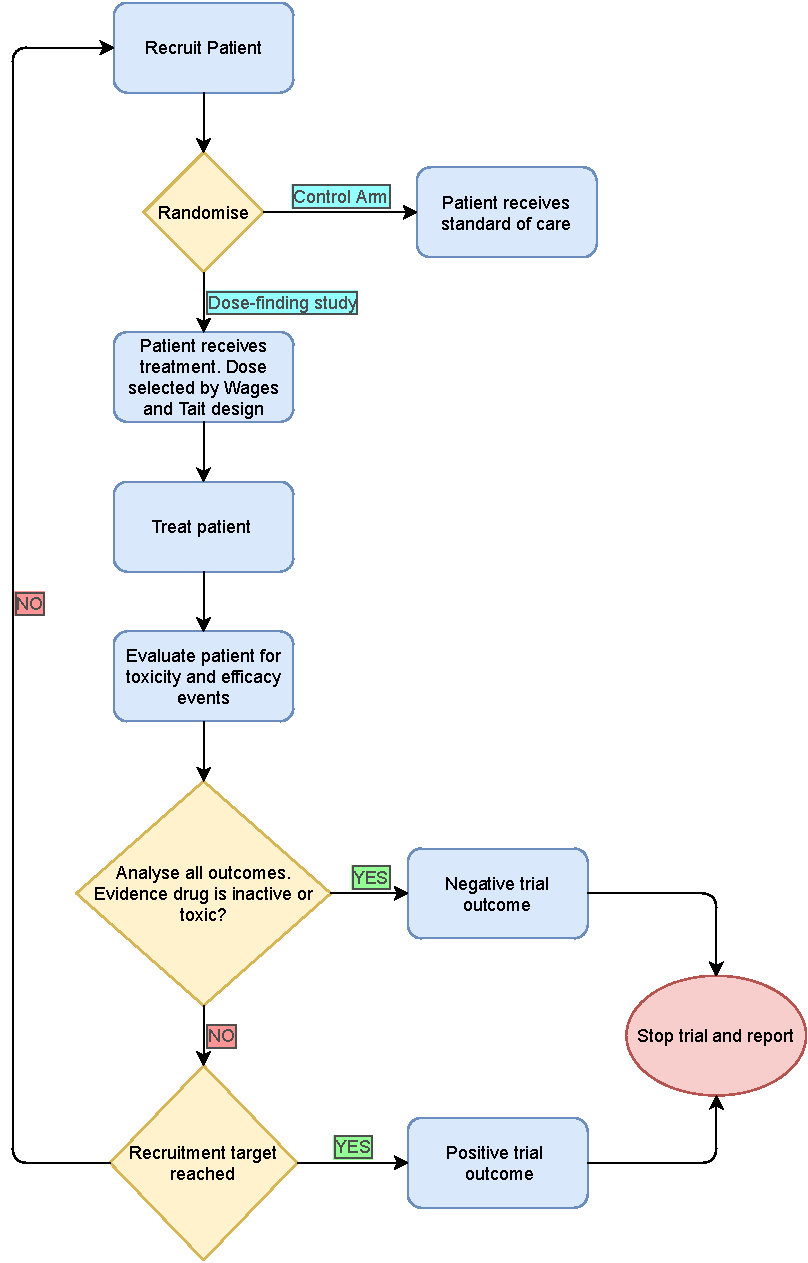
\includegraphics[width=0.77\textwidth]{WT-TwoArmExample}
\end{figure}

There is another approach that could also be used to include a control arm rather than our proposed design RtC-WT. A two-arm randomised design could be used where patients are allocated to either a control arm or a dose-finding arm. Those patients allocated in the dose-finding arm will then be a part of the WT design see Figure \ref{fig_wt:TwoArmExample}. This approach maintains many of the traditional qualities of a two-arm randomised trial. The number of patients in each arm can be specified this way and we guarantee a minimum number of patients in our control arm. Also, the characteristics of patients in both arms are likely to be similar which would be beneficial when making comparisons between the two arms. A downside of this method is that the data for control patients are no longer included in the modelling process. Whilst control patients may still be observed for efficacious and toxic events these won't be included in the modelling as such the ability to make inferences on the dose-toxicity and efficacy relationships in reference to a control/ standard of care dose is lost. 

Both of these approaches have their merit but also have flaws as well. RtC-WT is somewhat of a middle ground that aims to recruit patients to a control dose and include the control patients' data in the modelling process all whilst maintaining reasonable operating characteristics. We detail RtC-WT in Section \ref{WT:Design-RtC-WT} and explore the operating characteristics of this design in Section \ref{WT:Evaluation-of-the-Extension}.

%-----------------------------------
%	SUBSECTION 3.2
%-----------------------------------
\subsection{Design of the Proposed Extension RtC-WT}
\label{WT:Design-RtC-WT}

With this extension, much of the Wages and Tait design stays the same. The modification only impacts the adaptive randomisation (AR) phase and requires some additional specifications at the start of the trial. Firstly, we set the lowest dose-level $d_1$ to be the control dose-level. This dose-level should be included in the working models for efficacy and toxicity and should be treated like any other dose-level. Even if toxicity and efficacy events are expected to be non-existent for control their corresponding skeleton values must be non-zero. Investigators also need to consider a randomisation probability $\phi_R$ for the control dose. During the AR phase, $\phi_R$ represents the probability of selecting the control dose as the next dose level. The probability of randomisation $R_i$ for other dose in $\mathscrsfs{A}_j$ is scaled accordingly such that the $\sum_{d_i \in \mathscrsfs{A}_j} R_i = 1$. The adaptive randomisation probabilities can now be expressed as 

\begin{equation}
	R_1 = \phi_R,
\end{equation}

\begin{equation}
	R_i = (1-\phi_R)\frac{\hat{\pi}_E(d_i)}{\sum_{d_i \in \mathscrsfs{A}_j}\hat{\pi}_E(d_i)}, \; \; i=2,...,I. 
\end{equation}

Compared to Equation \ref{WT:eq_WT-ARprob} the adaptive randomisation probability is fixed to $\phi_R$ at the lowest dose (the control dose) and for all other dose levels in the admissible set $\mathscrsfs{A}_j$ a scaled randomisation probability is calculated. By fixing the probability for the control dose we guarantee a greater chance of patients being allocated to this dose-level. Although estimates of efficacy at the control dose-level $\hat{\pi}_E(d_1)$ do not directly impact its associated randomisation probability, the efficacy data that generated the estimate is still included in the efficacy modelling and impacts probabilities for the remaining dose-levels. Also, by scaling the remaining probabilities of dose-levels in the admissible set we ensure that those doses with high estimates of efficacy maintain their proportional advantage of selection over the other non-control doses.

Some adjustments were made to the stopping rule for safety. The WT design assesses the lower bound of the 95\% binomial confidence interval of DLT rate for the lowest dose to determine whether or not the trial should be stopped. However, with the RtC-WT design since the lowest dose is the control, it makes little sense to surmise treatment is toxic here since none of the patients on control would have received the experimental treatment. It is also likely the trial would never recommend stopping even if the treatment is toxic since patients on control are unlikely to experience a toxic event. The RtC-WT design stops for safety by checking for excess toxicity at the second-lowest dose-level (the first treatment dose-level).

Once the AR phase ends, dose-levels are no longer selected by adaptive randomisation. At this point, it will be difficult for patients to be recruited to the control dose since recommended doses will be based on those with the greatest estimates of efficacy. As such it is important to consider the values set for both your randomisation probability for control $\phi_R$ and the size of the AR phase $j_R$. Wages and Tait simply suggest a 50:50 split between both the AR phase and the maximisation phase and show relatively good performance at this level. However, for RtC-WT the AR phase is the main component and more thought should be given here. In the next section, we explore multiple combinations to better understand how these choices impact the operating characteristics of the design. We also compare RtC-WT to the two alternative designs mentioned in section  \ref{WT:Rationale-for-RtC-WT} via simulations and the inspection of operating characteristics specifically, the selection probabilities of the OBD and patient allocation numbers at each dose-level. 

%----------------------------------------------------------------------------------------
%	SECTION 4
%----------------------------------------------------------------------------------------
\section{Evaluation and Exploration of the Extension via Simulations}
\label{WT:Evaluation-of-the-Extension}

In this section, we evaluate the performance of RtC-WT in comparison to the two alternative designs mentioned in Section \ref{WT:Rationale-for-RtC-WT}. We also explore the impact of changing the probability of randomisation to control and the number of patients included in the adaptive randomisation phase. These will both be assessed via simulation and inspection of their operating characteristics. To facilitate simulations a generic trial example will be utilised along with a variety of scenarios. 

%-----------------------------------
%	SUBSECTION 4.1
%-----------------------------------
\subsection{Design Specification}
\label{WT:Design-Spec}

Here we detail the design specifications for RtC-WT that we will be using throughout this section. We assume five dose-levels, where the lowest dose is considered to be the control dose-level. The maximum sample size of the trial is set at 60 with patients recruited in cohorts of three and the first cohort starting at dose-level two (the first treatment dose-level). The pre-specified toxicity upper bound and efficacy lower bound are set at $\phi_T = 0.35$ and $\phi_E = 0.50$ respectively. Toxicity and efficacy skeletons, $p_i$ and $q_i$ respectively, are presented in Table \ref{tab_wt:tox-eff-skeleton}. In terms of efficacy relationships monotonic, unimodal and plateau skeletons were all used. We assume that each of the seven efficacy skeletons is equally likely and set $\upsilon(k) = \frac{1}{7}$. 


\begin{table}[!h]
	\centering
	\caption{Toxicity and efficacy skeletons for RtC-WT in the example trial.}
	\label{tab_wt:tox-eff-skeleton}
	\begin{tabular}{c|ccccc}
		\hline
		\multicolumn{1}{c|}{\multirow{2}{*}{\textbf{Skeleton}}} & \multicolumn{5}{c}{\textbf{Dose-levels}}                       \\
		\multicolumn{1}{c|}{}                                   & \textbf{1} & \textbf{2} & \textbf{3} & \textbf{4} & \textbf{5} \\ \hline
		$p_i$    & 0.1 & 0.15 & 0.25 & 0.35 & 0.45 \\
		$q_{i1}$ & 0.3 & 0.7 & 0.6 & 0.5 & 0.4 \\
		$q_{i2}$ & 0.3 & 0.6 & 0.7 & 0.6 & 0.5 \\
		$q_{i3}$ & 0.3 & 0.5 & 0.6 & 0.7 & 0.6 \\
		$q_{i4}$ & 0.3 & 0.4 & 0.5 & 0.6 & 0.7 \\
		$q_{i5}$ & 0.3 & 0.5 & 0.6 & 0.7 & 0.7 \\
		$q_{i6}$ & 0.3 & 0.6 & 0.7 & 0.7 & 0.7 \\
		$q_{i7}$ & 0.3 & 0.7 & 0.7 & 0.7 & 0.7 \\ \hline
	\end{tabular}
\end{table}

For the control dose, we have set our prior beliefs for the probability of toxicity at 10\% and the probability of efficacy at 30\%. This can of course be adjusted if there is reason to believe that the control dose may be slightly more/less effective or toxic. 

Wages and Tait recommend $(2I-1)$ efficacy skeletons be used which in this example would be nine, however, we have only considered seven. As there are only four active doses and we are assuming we understand the control dose in terms of toxicity and probability then seven different skeletons fits in the Wages and Tait's recommendation. Since we don't expect many efficacy events from our lowest dose we removed the two efficacy skeletons with dose-efficacy relationships that suggest the lowest dose would be the most efficacious. For completeness, the first extra skeleton would be unimodal with the highest efficacy occurring at dose-level one (i.e. 0.7, 0.6, 0.5, 0.4, 0.3 for dose-levels 1-5) and the second skeleton would be a plateau relationship with the plateau beginning at dose-level one (i.e. 0.7, 0.7, 0.7, 0.7, 0.7 for dose-levels 1-5). 

We also include the same stopping rules for safety and futility with the safety rule assessing toxicity at dose-level two. A rule will also be implemented to prevent the skipping of untried doses when escalating. This rule does not apply when de-escalating. 

The two parameters we have left to specify are the fixed adaptive randomisation probability for control $\phi_R$ and the number of patients included in the adaptive randomisation phase $j_R$. In Section \ref{WT:Design-RtC-WT} we briefly discussed the importance of giving thought when setting these values. This is due to the fact they are the main things driving how RtC-WT works compared to the standard WT design. For example, one could set the AR phase to last for the whole trial and keep a relatively low probability to randomise to control. Alternatively, the AR phase can be set for half the patients in the trial and double the probability of randomisation could be used. These two approaches could allocate the same number of patients in the control arm but have different operating characteristics. It could be hypothesised that by setting the AR phase for the whole trial you miss out on the maximisation phase where patients are allocated to the estimated most efficacious dose which could yield slightly worse operating characteristics. We explore different combinations of these parameters in the next section. 


%-----------------------------------
%	SUBSECTION 4.2
%-----------------------------------
\subsection{Impact of AR phase size and probability of randomisation to control on RtC-WT}
\label{WT:Impact-ARandRTCon-RtC-WT}


The effect of adjusting the probability of randomising to control $\phi_R$ is fairly intuitive, as the probability increases the percentage chance that patients are allocated to the control dose-level also increases. However, this is only in isolation without considering the size of the AR phase. Increasing the AR phase would also mean more patients are likely allocated to the control dose-level since the randomisation only occurs in the AR phase. The interest lies within the interaction of both of these components and their impacts on operating characteristics. To gain a better understanding of this impact on RtC-WT we consider multiple combinations. 

We look at two different probabilities for randomisation to control, $\phi_R = 0.2$ and $\phi_R = 0.33$ i.e. 20\% and 33\% probability of patients being allocated to the control dose-level during the AR phase of the trial. We also consider varying AR phase sizes, specifically $j_R = 0, 15, 30, 45 ,60$ essentially looking at when the AR phase lasts 0\%, 25\%, 50\%, 75\% and 100\% of the trial. The inclusion of setting the AR phase as 0 is somewhat counter-intuitive since the trial will just be run using the maximisation phase where the most efficacious doses are allocated. As such it is unlikely that the control dose-level would ever be the most efficacious specifically in our scenario here. However, its inclusion will serve as a benchmark as the design most likely to achieve optimal performance in terms of locating the OBD since there will be no randomisation and the estimated most efficacious dose will always be the one being tested. Similarly, by setting the AR phase at 60 we limit some of the designs features by never entering the maximisation phase to select dose levels based on efficacy. Also, the stopping rule for futility doesn't come into play. Although, many more combinations could be explored this set provide a good basis for us to gain a better understanding of how RtC-WT works. It also helps us understand how best to optimise RtC-WT for comparisons with alternative designs later on.  

To compare these different combinations we use simulations covering a wide range of scenarios. For each scenario, we simulate 10000 trials each consisting of 60 patients recruited in cohorts of three. Patient outcomes for toxicity and efficacy are randomly sampled using true toxicity and true efficacy probabilities, these are assumed to be independent of each other. Dose-allocation decisions are made after each cohort of patients and then the subsequent cohort is allocated the recommended dose. The trial could also be stopped here if the recruitment target is reached or if any of the stopping rules are triggered. The rest of the design specification is as defined in Section \ref{WT:Design-Spec}. 

The true toxicity and efficacy probabilities are manipulated to produce each scenario for the simulations. Table \ref{tab_wt:sim-scenarios} shows a summary of the scenarios that will be used. We look at a combination of five different efficacy curves with three toxicity curves giving 15 scenarios altogether. The five dose-efficacy relationships we consider are; monotonically increasing, unimodal (at dose level 3), plateau (starting at dose level 3), monotonically decreasing and finally no efficacy. For toxicity we look at scenarios where all doses are tolerable, all doses are toxic and a scenario where only higher doses (dose-levels 4 and 5) are toxic. We also list which doses would be considered the OBD under the designs specification along with which doses would be good for each of the scenarios. The OBD in this context would be the dose which maximises efficacy whilst not breaching the toxicity limit. Good doses are those which are considered safe (probability of toxicity $\leq$ 35\%) and efficacious (probability of efficacy $\geq$ 50\%). For scenarios that are too toxic/lack efficacy, we would expect the trial to stop early, here we have labelled the OBD as being the probability of stopping and good doses as the probability of stopping and selecting dose-level 1, the control dose. Whilst allocating patients to dose-level 1 in these scenarios is not necessarily a bad thing it would likely mean more patients are exposed to the toxic/inefficacious doses which is not optimal, hence the distinction.  

Operating characteristics for the scenarios under investigation are given in Table \ref{tab_wt:SelectProbCombos}. The table provides the following operating characteristics: 

\begin{itemize}
	\item P(OBD) - Probability of selecting the OBD
	\item P(Good) - Probability of selecting a good dose
	\item N(OBD) - Mean number of patients treated at the OBD
	\item N(Good) - Mean number of patients treated at good doses
	\item N(Control) - Mean number of patients treated at the control dose (dose-level 1)
\end{itemize}

These are provided for each scenario under the 10 different parameterisations of $\phi_R$ and $j_R$. For certain scenarios, where the ideal outcome would be to stop early, N(OBD) is left blank as patients aren't allocated to a specific dose. Also, for these scenarios N(Good) and N(Control) are the same as the only good dose patients can be allocated to is the control. Then for scenarios where there is only one good dose-level that would be the OBD as well so P(OBD) and P(Good) would be the same as would N(OBD) and N(Good). 

\newpage

\begin{table}[h!]
	\centering
	\caption{Summary of the efficacy and toxicity curves used in each scenario.}
	\label{tab_wt:sim-scenarios}
\resizebox{\textwidth}{!}{%
	\begin{tabular}{cc|ccccc|l|cc}
		\hline
		\multicolumn{2}{c|}{\textbf{Scenario}} & \textbf{1} & \textbf{2} & \textbf{3} & \textbf{4} & \textbf{5} & \textbf{Description} & \textbf{OBD} & \textbf{Good Dose} \\ \hline
		\multirow{2}{*}{1} & tox & 0.1 & 0.2 & 0.25 & 0.3 & 0.35 & All doses tolerable & \multirow{2}{*}{5} & \multirow{2}{*}{3-5} \\
		& eff & 0.3 & 0.4 & 0.5 & 0.6 & 0.7 & Monotone increasing &  &  \\ \hline
		\multirow{2}{*}{2} & tox & 0.1 & 0.45 & 0.5 & 0.55 & 0.6 & Too toxic & \multirow{2}{*}{Stop} & \multirow{2}{*}{Stop/Control} \\
		& eff & 0.3 & 0.4 & 0.5 & 0.6 & 0.7 & Monotone increasing &  &  \\ \hline
		\multirow{2}{*}{3} & tox & 0.1 & 0.25 & 0.35 & 0.45 & 0.55 & High doses toxic & \multirow{2}{*}{3} & \multirow{2}{*}{3} \\
		& eff & 0.3 & 0.4 & 0.5 & 0.6 & 0.7 & Monotone increasing &  &  \\ \hline
		\multirow{2}{*}{4} & tox & 0.1 & 0.2 & 0.25 & 0.3 & 0.35 & All doses tolerable & \multirow{2}{*}{3} & \multirow{2}{*}{3-4} \\
		& eff & 0.3 & 0.4 & 0.7 & 0.5 & 0.4 & Unimodal &  &  \\ \hline
		\multirow{2}{*}{5} & tox & 0.1 & 0.45 & 0.5 & 0.55 & 0.6 & Too toxic & \multirow{2}{*}{Stop} & \multirow{2}{*}{Stop/Control} \\
		& eff & 0.3 & 0.4 & 0.7 & 0.5 & 0.4 & Unimodal &  &  \\ \hline
		\multirow{2}{*}{6} & tox & 0.1 & 0.25 & 0.35 & 0.45 & 0.55 & High doses toxic & \multirow{2}{*}{3} & \multirow{2}{*}{3} \\
		& eff & 0.3 & 0.4 & 0.7 & 0.5 & 0.4 & Unimodal &  &  \\ \hline
		\multirow{2}{*}{7} & tox & 0.1 & 0.2 & 0.25 & 0.3 & 0.35 & All doses tolerable & \multirow{2}{*}{3} & \multirow{2}{*}{3-5} \\
		& eff & 0.3 & 0.4 & 0.6 & 0.6 & 0.6 & Plateau &  &  \\ \hline
		\multirow{2}{*}{8} & tox & 0.1 & 0.45 & 0.5 & 0.55 & 0.6 & Too toxic & \multirow{2}{*}{Stop} & \multirow{2}{*}{Stop/Control} \\
		& eff & 0.3 & 0.4 & 0.6 & 0.6 & 0.6 & Plateau &  &  \\ \hline
		\multirow{2}{*}{9} & tox & 0.1 & 0.25 & 0.35 & 0.45 & 0.55 & High doses toxic & \multirow{2}{*}{3} & \multirow{2}{*}{3} \\
		& eff & 0.3 & 0.4 & 0.6 & 0.6 & 0.6 & Plateau &  &  \\ \hline
		\multirow{2}{*}{10} & tox & 0.1 & 0.2 & 0.25 & 0.3 & 0.35 & All doses tolerable & \multirow{2}{*}{2} & \multirow{2}{*}{2-4} \\
		& eff & 0.3 & 0.7 & 0.6 & 0.5 & 0.4 & Monotone decreasing &  &  \\ \hline
		\multirow{2}{*}{11} & tox & 0.1 & 0.45 & 0.5 & 0.55 & 0.6 & Too toxic & \multirow{2}{*}{Stop} & \multirow{2}{*}{Stop/Control} \\
		& eff & 0.3 & 0.7 & 0.6 & 0.5 & 0.4 & Monotone decreasing &  &  \\ \hline
		\multirow{2}{*}{12} & tox & 0.1 & 0.25 & 0.35 & 0.45 & 0.55 & High doses toxic & \multirow{2}{*}{2} & \multirow{2}{*}{2-3} \\
		& eff & 0.3 & 0.7 & 0.6 & 0.5 & 0.4 & Monotone decreasing &  &  \\ \hline
		\multirow{2}{*}{13} & tox & 0.1 & 0.2 & 0.25 & 0.3 & 0.35 & All doses tolerable & \multirow{2}{*}{Stop} & \multirow{2}{*}{Stop/Control} \\
		& eff & 0.3 & 0.3 & 0.3 & 0.3 & 0.3 & No Efficacy &  &  \\ \hline
		\multirow{2}{*}{14} & tox & 0.1 & 0.45 & 0.5 & 0.55 & 0.6 & Too toxic & \multirow{2}{*}{Stop} & \multirow{2}{*}{Stop/Control} \\
		& eff & 0.3 & 0.3 & 0.3 & 0.3 & 0.3 & No Efficacy &  &  \\ \hline
		\multirow{2}{*}{15} & tox & 0.1 & 0.25 & 0.35 & 0.45 & 0.55 & High doses toxic & \multirow{2}{*}{Stop} & \multirow{2}{*}{Stop/Control} \\
		& eff & 0.3 & 0.3 & 0.3 & 0.3 & 0.3 & No Efficacy &  &  \\ \hline
	\end{tabular}%
}
\end{table}

\newpage

\setlength\LTcapwidth{\textwidth}
\begingroup\fontsize{9}{11}\selectfont

\begin{longtable}[h!]{cccccccccc}
		
	\caption[Operating characteristics for multiple combinations of parameters.]{\label{tab_wt:SelectProbCombos}Operating characteristics for multiple combinations of AR phase size and probabilities for randomisation to control. Probability of selecting the OBD or good dose levels, mean number of patients treated at those dose levels and at the control dose after 10000 simulations.}\\
	\toprule
	Scenario & $\phi_R$ & $j_R$ & OBD & Good Doses & P(OBD) & P(Good) & N(OBD) & N(Good) & N(Control)\\
	\midrule
	\endfirsthead
	\caption[]{Operating characteristics (continued)}\\
	\toprule
	Scenario & \ $\phi_R$ & $j_R$ & OBD & Good Doses & P(OBD) & P(Good) & N(OBD) & N(Good) & N(Control)\\
	\midrule
	\endhead
	
	\endfoot
	\bottomrule
	\endlastfoot
 &  & 0 & 5 & 3-5 & 0.05 & 0.60 & 2.8 & 32.1 & 1.2\\
\nopagebreak
&  & 15 & 5 & 3-5 & 0.05 & 0.65 & 2.7 & 32 & 3.6\\
\nopagebreak
&  & 30 & 5 & 3-5 & 0.05 & 0.71 & 2.2 & 31.1 & 6.4\\
\nopagebreak
&  & 45 & 5 & 3-5 & 0.05 & 0.76 & 1.5 & 27.5 & 9.4\\
\nopagebreak
& \multirow{-5}{*}{\centering\arraybackslash 0.2} & 60 & 5 & 3-5 & 0.04 & 0.80 & 1.1 & 22.9 & 12.4\\
\nopagebreak
&  & 0 & 5 & 3-5 & 0.05 & 0.60 & 2.8 & 32.1 & 1.2\\
\nopagebreak
&  & 15 & 5 & 3-5 & 0.07 & 0.67 & 3.1 & 32.6 & 4.9\\
\nopagebreak
&  & 30 & 5 & 3-5 & 0.06 & 0.75 & 2.2 & 30.4 & 9.8\\
\nopagebreak
&  & 45 & 5 & 3-5 & 0.05 & 0.79 & 1.3 & 25.5 & 14.7\\
\nopagebreak
\multirow{-10}{*}{\centering\arraybackslash 1} & \multirow{-5}{*}{\centering\arraybackslash 0.33} & 60 & 5 & 3-5 & 0.03 & 0.82 & 0.8 & 19.4 & 19.6\\
\cmidrule{1-10}\pagebreak[0]
&  & 0 & stop & stop/1 & 0.81 & 0.85 & - & 10.1 & 10.1\\
\nopagebreak
&  & 15 & stop & stop/1 & 0.80 & 0.85 & - & 11 & 11\\
\nopagebreak
&  & 30 & stop & stop/1 & 0.77 & 0.81 & - & 13.2 & 13.2\\
\nopagebreak
&  & 45 & stop & stop/1 & 0.72 & 0.75 & - & 15.6 & 15.6\\
\nopagebreak
& \multirow{-5}{*}{\centering\arraybackslash 0.2} & 60 & stop & stop/1 & 0.41 & 0.50 & - & 17.9 & 17.9\\
\nopagebreak
&  & 0 & stop & stop/1 & 0.81 & 0.85 & - & 10.1 & 10.1\\
\nopagebreak
&  & 15 & stop & stop/1 & 0.77 & 0.83 & - & 11.4 & 11.4\\
\nopagebreak
&  & 30 & stop & stop/1 & 0.75 & 0.79 & - & 14 & 14\\
\nopagebreak
&  & 45 & stop & stop/1 & 0.67 & 0.70 & - & 17.6 & 17.6\\
\nopagebreak
\multirow{-10}{*}{\centering\arraybackslash 2} & \multirow{-5}{*}{\centering\arraybackslash 0.33} & 60 & stop & stop/1 & 0.38 & 0.42 & - & 20.7 & 20.7\\
\cmidrule{1-10}\pagebreak[0]
&  & 0 & 3 & 3 & 0.25 & 0.25 & 15.5 & 15.5 & 2.6\\
\nopagebreak
&  & 15 & 3 & 3 & 0.31 & 0.31 & 16.8 & 16.8 & 4.7\\
\nopagebreak
&  & 30 & 3 & 3 & 0.35 & 0.35 & 16.8 & 16.8 & 7.5\\
\nopagebreak
&  & 45 & 3 & 3 & 0.42 & 0.42 & 15.5 & 15.5 & 10.4\\
\nopagebreak
& \multirow{-5}{*}{\centering\arraybackslash 0.2} & 60 & 3 & 3 & 0.48 & 0.48 & 12.7 & 12.7 & 13.3\\
\nopagebreak
&  & 0 & 3 & 3 & 0.25 & 0.25 & 15.5 & 15.5 & 2.6\\
\nopagebreak
&  & 15 & 3 & 3 & 0.32 & 0.32 & 17.2 & 17.2 & 5.8\\
\nopagebreak
&  & 30 & 3 & 3 & 0.39 & 0.39 & 17.3 & 17.3 & 10.4\\
\nopagebreak
&  & 45 & 3 & 3 & 0.46 & 0.46 & 15.2 & 15.2 & 15.2\\
\nopagebreak
\multirow{-10}{*}{\centering\arraybackslash 3} & \multirow{-5}{*}{\centering\arraybackslash 0.33} & 60 & 3 & 3 & 0.52 & 0.52 & 11.5 & 11.5 & 20.1\\
\cmidrule{1-10}\pagebreak[0]
&  & 0 & 3 & 3-4 & 0.69 & 0.75 & 32.3 & 37.2 & 1.3\\
\nopagebreak
&  & 15 & 3 & 3-4 & 0.69 & 0.76 & 30.3 & 35.5 & 3.5\\
\nopagebreak
&  & 30 & 3 & 3-4 & 0.71 & 0.81 & 26.4 & 32.3 & 6.5\\
\nopagebreak
&  & 45 & 3 & 3-4 & 0.73 & 0.83 & 21.6 & 27.4 & 9.5\\
\nopagebreak
& \multirow{-5}{*}{\centering\arraybackslash 0.2} & 60 & 3 & 3-4 & 0.71 & 0.83 & 16 & 21.7 & 12.4\\
\nopagebreak
&  & 0 & 3 & 3-4 & 0.69 & 0.75 & 32.3 & 37.2 & 1.3\\
\nopagebreak
&  & 15 & 3 & 3-4 & 0.69 & 0.77 & 29.5 & 35.1 & 5\\
\nopagebreak
&  & 30 & 3 & 3-4 & 0.70 & 0.81 & 24.8 & 31 & 9.9\\
\nopagebreak
&  & 45 & 3 & 3-4 & 0.70 & 0.84 & 19.7 & 25.4 & 14.7\\
\nopagebreak
\multirow{-10}{*}{\centering\arraybackslash 4} & \multirow{-5}{*}{\centering\arraybackslash 0.33} & 60 & 3 & 3-4 & 0.68 & 0.83 & 13.7 & 18.5 & 19.5\\
\cmidrule{1-10}\pagebreak[0]
&  & 0 & stop & stop/1 & 0.81 & 0.86 & - & 10.1 & 10.1\\
\nopagebreak
&  & 15 & stop & stop/1 & 0.79 & 0.84 & - & 11.1 & 11.1\\
\nopagebreak
&  & 30 & stop & stop/1 & 0.77 & 0.82 & - & 13.1 & 13.1\\
\nopagebreak
&  & 45 & stop & stop/1 & 0.71 & 0.75 & - & 15.6 & 15.6\\
\nopagebreak
& \multirow{-5}{*}{\centering\arraybackslash 0.2} & 60 & stop & stop/1 & 0.41 & 0.49 & - & 17.9 & 17.9\\
\nopagebreak
&  & 0 & stop & stop/1 & 0.81 & 0.86 & - & 10.1 & 10.1\\
\nopagebreak
&  & 15 & stop & stop/1 & 0.78 & 0.83 & - & 11.3 & 11.3\\
\nopagebreak
&  & 30 & stop & stop/1 & 0.75 & 0.78 & - & 14.1 & 14.1\\
\nopagebreak
&  & 45 & stop & stop/1 & 0.67 & 0.70 & - & 17.6 & 17.6\\
\nopagebreak
\multirow{-10}{*}{\centering\arraybackslash 5} & \multirow{-5}{*}{\centering\arraybackslash 0.33} & 60 & stop & stop/1 & 0.38 & 0.43 & - & 20.8 & 20.8\\
\cmidrule{1-10}\pagebreak[0]
&  & 0 & 3 & 3 & 0.37 & 0.37 & 21.2 & 21.2 & 2.6\\
\nopagebreak
&  & 15 & 3 & 3 & 0.41 & 0.41 & 21.3 & 21.3 & 4.5\\
\nopagebreak
&  & 30 & 3 & 3 & 0.45 & 0.45 & 19.6 & 19.6 & 7.5\\
\nopagebreak
&  & 45 & 3 & 3 & 0.50 & 0.50 & 17.1 & 17.1 & 10.4\\
\nopagebreak
& \multirow{-5}{*}{\centering\arraybackslash 0.2} & 60 & 3 & 3 & 0.54 & 0.54 & 12.8 & 12.8 & 13.4\\
\nopagebreak
&  & 0 & 3 & 3 & 0.37 & 0.37 & 21.2 & 21.2 & 2.6\\
\nopagebreak
&  & 15 & 3 & 3 & 0.42 & 0.42 & 21.4 & 21.4 & 5.8\\
\nopagebreak
&  & 30 & 3 & 3 & 0.50 & 0.50 & 20.3 & 20.3 & 10.4\\
\nopagebreak
&  & 45 & 3 & 3 & 0.55 & 0.55 & 16.6 & 16.6 & 15.1\\
\nopagebreak
\multirow{-10}{*}{\centering\arraybackslash 6} & \multirow{-5}{*}{\centering\arraybackslash 0.33} & 60 & 3 & 3 & 0.59 & 0.59 & 11.5 & 11.5 & 20.1\\
\cmidrule{1-10}\pagebreak[0]
&  & 0 & 3 & 3-5 & 0.48 & 0.70 & 23.9 & 35.6 & 1.3\\
\nopagebreak
&  & 15 & 3 & 3-5 & 0.50 & 0.73 & 23.7 & 35 & 3.5\\
\nopagebreak
&  & 30 & 3 & 3-5 & 0.52 & 0.78 & 21.8 & 32.4 & 6.4\\
\nopagebreak
&  & 45 & 3 & 3-5 & 0.56 & 0.81 & 19.3 & 27.9 & 9.4\\
\nopagebreak
& \multirow{-5}{*}{\centering\arraybackslash 0.2} & 60 & 3 & 3-5 & 0.57 & 0.82 & 15.8 & 22.5 & 12.5\\
\nopagebreak
&  & 0 & 3 & 3-5 & 0.48 & 0.70 & 23.9 & 35.6 & 1.3\\
\nopagebreak
&  & 15 & 3 & 3-5 & 0.49 & 0.75 & 22.7 & 35.1 & 5\\
\nopagebreak
&  & 30 & 3 & 3-5 & 0.51 & 0.80 & 20.8 & 31.6 & 9.7\\
\nopagebreak
&  & 45 & 3 & 3-5 & 0.55 & 0.84 & 17.7 & 26 & 14.7\\
\nopagebreak
\multirow{-10}{*}{\centering\arraybackslash 7} & \multirow{-5}{*}{\centering\arraybackslash 0.33} & 60 & 3 & 3-5 & 0.56 & 0.84 & 13.7 & 19.6 & 19.5\\
\cmidrule{1-10}\pagebreak[0]
&  & 0 & stop & stop/1 & 0.81 & 0.85 & - & 10.2 & 10.2\\
\nopagebreak
&  & 15 & stop & stop/1 & 0.79 & 0.84 & - & 11.1 & 11.1\\
\nopagebreak
&  & 30 & stop & stop/1 & 0.77 & 0.81 & - & 13.2 & 13.2\\
\nopagebreak
&  & 45 & stop & stop/1 & 0.71 & 0.76 & - & 15.6 & 15.6\\
\nopagebreak
& \multirow{-5}{*}{\centering\arraybackslash 0.2} & 60 & stop & stop/1 & 0.41 & 0.50 & - & 17.9 & 17.9\\
\nopagebreak
&  & 0 & stop & stop/1 & 0.81 & 0.85 & - & 10.2 & 10.2\\
\nopagebreak
&  & 15 & stop & stop/1 & 0.78 & 0.82 & - & 11.3 & 11.3\\
\nopagebreak
&  & 30 & stop & stop/1 & 0.75 & 0.79 & - & 14 & 14\\
\nopagebreak
&  & 45 & stop & stop/1 & 0.69 & 0.71 & - & 17.4 & 17.4\\
\nopagebreak
\multirow{-10}{*}{\centering\arraybackslash 8} & \multirow{-5}{*}{\centering\arraybackslash 0.33} & 60 & stop & stop/1 & 0.38 & 0.43 & - & 20.8 & 20.8\\
\cmidrule{1-10}\pagebreak[0]
&  & 0 & 3 & 3 & 0.34 & 0.34 & 18.6 & 18.6 & 2.6\\
\nopagebreak
&  & 15 & 3 & 3 & 0.36 & 0.36 & 19.2 & 19.2 & 4.6\\
\nopagebreak
&  & 30 & 3 & 3 & 0.42 & 0.42 & 18.3 & 18.3 & 7.5\\
\nopagebreak
&  & 45 & 3 & 3 & 0.45 & 0.45 & 16.3 & 16.3 & 10.3\\
\nopagebreak
& \multirow{-5}{*}{\centering\arraybackslash 0.2} & 60 & 3 & 3 & 0.50 & 0.50 & 12.9 & 12.9 & 13.3\\
\nopagebreak
&  & 0 & 3 & 3 & 0.34 & 0.34 & 18.6 & 18.6 & 2.6\\
\nopagebreak
&  & 15 & 3 & 3 & 0.38 & 0.38 & 19.7 & 19.7 & 5.9\\
\nopagebreak
&  & 30 & 3 & 3 & 0.45 & 0.45 & 18.6 & 18.6 & 10.4\\
\nopagebreak
&  & 45 & 3 & 3 & 0.52 & 0.52 & 15.9 & 15.9 & 15.2\\
\nopagebreak
\multirow{-10}{*}{\centering\arraybackslash 9} & \multirow{-5}{*}{\centering\arraybackslash 0.33} & 60 & 3 & 3 & 0.56 & 0.56 & 11.5 & 11.5 & 20.1\\
\cmidrule{1-10}\pagebreak[0]
&  & 0 & 2 & 2-4 & 0.77 & 0.97 & 45.1 & 57.1 & 1.3\\
\nopagebreak
&  & 15 & 2 & 2-4 & 0.79 & 0.97 & 41.8 & 55.3 & 3.5\\
\nopagebreak
&  & 30 & 2 & 2-4 & 0.79 & 0.98 & 37.2 & 52.5 & 6.5\\
\nopagebreak
&  & 45 & 2 & 2-4 & 0.79 & 0.99 & 32.2 & 49.6 & 9.4\\
\nopagebreak
& \multirow{-5}{*}{\centering\arraybackslash 0.2} & 60 & 2 & 2-4 & 0.80 & 0.99 & 26.4 & 46.4 & 12.3\\
\nopagebreak
&  & 0 & 2 & 2-4 & 0.77 & 0.97 & 45.1 & 57.1 & 1.3\\
\nopagebreak
&  & 15 & 2 & 2-4 & 0.77 & 0.97 & 40.1 & 53.6 & 5\\
\nopagebreak
&  & 30 & 2 & 2-4 & 0.76 & 0.98 & 34.6 & 49.1 & 9.8\\
\nopagebreak
&  & 45 & 2 & 2-4 & 0.76 & 0.99 & 28.4 & 44.3 & 14.7\\
\nopagebreak
\multirow{-10}{*}{\centering\arraybackslash 10} & \multirow{-5}{*}{\centering\arraybackslash 0.33} & 60 & 2 & 2-4 & 0.78 & 0.99 & 22.3 & 39.2 & 19.6\\
\cmidrule{1-10}\pagebreak[0]
&  & 0 & stop & stop/1 & 0.65 & 0.74 & - & 11.7 & 11.7\\
\nopagebreak
&  & 15 & stop & stop/1 & 0.65 & 0.72 & - & 12.3 & 12.3\\
\nopagebreak
&  & 30 & stop & stop/1 & 0.62 & 0.69 & - & 13.8 & 13.8\\
\nopagebreak
&  & 45 & stop & stop/1 & 0.57 & 0.63 & - & 15.7 & 15.7\\
\nopagebreak
& \multirow{-5}{*}{\centering\arraybackslash 0.2} & 60 & stop & stop/1 & 0.41 & 0.49 & - & 17.9 & 17.9\\
\nopagebreak
&  & 0 & stop & stop/1 & 0.65 & 0.74 & - & 11.7 & 11.7\\
\nopagebreak
&  & 15 & stop & stop/1 & 0.64 & 0.72 & - & 12.5 & 12.5\\
\nopagebreak
&  & 30 & stop & stop/1 & 0.60 & 0.67 & - & 14.7 & 14.7\\
\nopagebreak
&  & 45 & stop & stop/1 & 0.52 & 0.56 & - & 17.7 & 17.7\\
\nopagebreak
\multirow{-10}{*}{\centering\arraybackslash 11} & \multirow{-5}{*}{\centering\arraybackslash 0.33} & 60 & stop & stop/1 & 0.38 & 0.42 & - & 20.9 & 20.9\\
\cmidrule{1-10}\pagebreak[0]
&  & 0 & 2 & 2-3 & 0.83 & 0.92 & 47.3 & 53.7 & 2.7\\
\nopagebreak
&  & 15 & 2 & 2-3 & 0.83 & 0.93 & 43.6 & 51.8 & 4.7\\
\nopagebreak
&  & 30 & 2 & 2-3 & 0.82 & 0.95 & 39.7 & 49.3 & 7.4\\
\nopagebreak
&  & 45 & 2 & 2-3 & 0.84 & 0.96 & 35.9 & 46.4 & 10.4\\
\nopagebreak
& \multirow{-5}{*}{\centering\arraybackslash 0.2} & 60 & 2 & 2-3 & 0.85 & 0.97 & 31.7 & 43.5 & 13.2\\
\nopagebreak
&  & 0 & 2 & 2-3 & 0.83 & 0.92 & 47.3 & 53.7 & 2.7\\
\nopagebreak
&  & 15 & 2 & 2-3 & 0.81 & 0.94 & 41.9 & 50.7 & 5.9\\
\nopagebreak
&  & 30 & 2 & 2-3 & 0.80 & 0.95 & 36.6 & 46.3 & 10.4\\
\nopagebreak
&  & 45 & 2 & 2-3 & 0.81 & 0.96 & 31.7 & 41.8 & 15.3\\
\nopagebreak
\multirow{-10}{*}{\centering\arraybackslash 12} & \multirow{-5}{*}{\centering\arraybackslash 0.33} & 60 & 2 & 2-3 & 0.82 & 0.97 & 26 & 36.8 & 20\\
\cmidrule{1-10}\pagebreak[0]
&  & 0 & stop & stop/1 & 0.82 & 0.82 & - & 1.2 & 1.2\\
\nopagebreak
&  & 15 & stop & stop/1 & 0.78 & 0.78 & - & 3.5 & 3.5\\
\nopagebreak
&  & 30 & stop & stop/1 & 0.70 & 0.70 & - & 6.5 & 6.5\\
\nopagebreak
&  & 45 & stop & stop/1 & 0.57 & 0.57 & - & 9.5 & 9.5\\
\nopagebreak
& \multirow{-5}{*}{\centering\arraybackslash 0.2} & 60 & stop & stop/1 & 0.01 & 0.01 & - & 12.4 & 12.4\\
\nopagebreak
&  & 0 & stop & stop/1 & 0.82 & 0.82 & - & 1.2 & 1.2\\
\nopagebreak
&  & 15 & stop & stop/1 & 0.76 & 0.76 & - & 4.9 & 4.9\\
\nopagebreak
&  & 30 & stop & stop/1 & 0.68 & 0.68 & - & 9.7 & 9.7\\
\nopagebreak
&  & 45 & stop & stop/1 & 0.54 & 0.54 & - & 14.7 & 14.7\\
\nopagebreak
\multirow{-10}{*}{\centering\arraybackslash 13} & \multirow{-5}{*}{\centering\arraybackslash 0.33} & 60 & stop & stop/1 & 0.01 & 0.01 & - & 19.6 & 19.6\\
\cmidrule{1-10}\pagebreak[0]
&  & 0 & stop & stop/1 & 0.96 & 0.97 & - & 8.3 & 8.3\\
\nopagebreak
&  & 15 & stop & stop/1 & 0.95 & 0.96 & - & 9.6 & 9.6\\
\nopagebreak
&  & 30 & stop & stop/1 & 0.94 & 0.95 & - & 12.4 & 12.4\\
\nopagebreak
&  & 45 & stop & stop/1 & 0.92 & 0.93 & - & 15.5 & 15.5\\
\nopagebreak
& \multirow{-5}{*}{\centering\arraybackslash 0.2} & 60 & stop & stop/1 & 0.42 & 0.50 & - & 17.7 & 17.7\\
\nopagebreak
&  & 0 & stop & stop/1 & 0.96 & 0.97 & - & 8.3 & 8.3\\
\nopagebreak
&  & 15 & stop & stop/1 & 0.95 & 0.96 & - & 9.9 & 9.9\\
\nopagebreak
&  & 30 & stop & stop/1 & 0.93 & 0.94 & - & 13.5 & 13.5\\
\nopagebreak
&  & 45 & stop & stop/1 & 0.89 & 0.90 & - & 17.3 & 17.3\\
\nopagebreak
\multirow{-10}{*}{\centering\arraybackslash 14} & \multirow{-5}{*}{\centering\arraybackslash 0.33} & 60 & stop & stop/1 & 0.38 & 0.43 & - & 20.8 & 20.8\\
\cmidrule{1-10}\pagebreak[0]
&  & 0 & stop & stop/1 & 0.89 & 0.89 & - & 2.3 & 2.3\\
\nopagebreak
&  & 15 & stop & stop/1 & 0.87 & 0.87 & - & 4.5 & 4.5\\
\nopagebreak
&  & 30 & stop & stop/1 & 0.82 & 0.82 & - & 7.3 & 7.3\\
\nopagebreak
&  & 45 & stop & stop/1 & 0.73 & 0.73 & - & 10.4 & 10.4\\
\nopagebreak
& \multirow{-5}{*}{\centering\arraybackslash 0.2} & 60 & stop & stop/1 & 0.02 & 0.03 & - & 13.4 & 13.4\\
\nopagebreak
&  & 0 & stop & stop/1 & 0.89 & 0.89 & - & 2.3 & 2.3\\
\nopagebreak
&  & 15 & stop & stop/1 & 0.86 & 0.86 & - & 5.7 & 5.7\\
\nopagebreak
&  & 30 & stop & stop/1 & 0.80 & 0.80 & - & 10.3 & 10.3\\
\nopagebreak
&  & 45 & stop & stop/1 & 0.69 & 0.70 & - & 15.2 & 15.2\\
\nopagebreak
\multirow{-10}{*}{\centering\arraybackslash 15} & \multirow{-5}{*}{\centering\arraybackslash 0.33} & 60 & stop & stop/1 & 0.02 & 0.03 & - & 20.1 & 20.1\\*
\end{longtable}
\endgroup{}

\newpage

For scenario 1 it is relatively simple to select an admissible dose since all doses are tolerable and efficacy increases monotonically. The difficulty is locating the OBD. All of these combinations fail to identify the OBD (dose-level 5) more than 7\% of the time. Whereas the probability of selecting a good dose is between 60 and 82\%. As the size of the AR phase increases from 0 to 60 so do the selection probabilities for a good dose, going from 60\% to 80\% and 60\% to 82\% for randomisation probabilities of 0.2 and 0.33 respectively. It should be noted that the two designs with no AR phase are identical since the randomisation probabilities are never used. In terms of the number of patients treated we see more patients in the control arm as AR phase size and randomisation probability increase. This is expected since if you increase the amount of time available for cohorts to be randomised or the probability in which that is done, more patients will be recruited to control. By increasing the probability of randomising to control we can also see that fewer patients are being treated at good doses at higher AR sizes. Also, the $\phi_R$ figure does not guarantee that exact percentage of patients in the control dose will be allocated to control but for this scenario, it appears to be somewhat accurate. 

Scenario 2 has no OBD as all treatment doses are considered toxic. For most of the combinations, stopping occurs 67-81\% of the time and including allocation to the control arm we see this increase to 70-85\%. Slightly concerning is the case where the AR phase lasts the whole trial. Here stopping is less frequent at 50\% and 42\% for probabilities of randomisation to control of $\phi_R = 0.2$ and $\phi_R = 0.33$ respectively. To understand why this was occurring we investigated the failure mechanism in individual simulation runs. We found that the design was stopping appropriately for excess toxicity. However, due to setting the AR phase at 60 the maximisation phase never starts and thus the stopping rule for futility never triggers. This is why this parametrisation performs worse comparatively. Even though this scenario is to check for excess toxicity the true efficacy rates used in this scenario could also potentially trigger the futility rule as they are set at 40\% and 50\% for dose-levels 2 and 3. To confirm this we ran some of the parametrisations where the AR size is less than 60 using a design without the futility rule and observed similar stopping rates of 40\% in this scenario. This indicates that overall our design is not that great at stopping for potential toxicities. This could be improved by utilising different stopping criteria. We also observe this difference in scenarios 5, 8, 11 and 14 where we should also be stopping for excess toxicity. The results for $j_R$ = 60 in these scenarios could be interpreted as our baseline for stopping for excess toxicity and the increase stopping in other parametrisations represent how often the futility rule is triggered.      

In scenario 3, the treatment is toxic at high doses and ineffective at lower doses meaning only one dose can be considered good or the OBD. This is a difficult scenario since only one of the five dose-levels is suitable to allocate patients to. The selection probabilities range from 25\% to 52\%. We see as $j_R$ increases selection probabilities also increase. As those designs with smaller AR phases go into the maximisation phase they would be selecting dose-levels based on those in the admissible set with higher efficacy. Since the doses with higher efficacy also have a high toxicity rate there is a chance early on in the trial this isn't detected resulting in toxicities at the higher dose-levels causing the trial to stop early. This could be a reason why the designs with the larger AR phase perform better as doses would be randomly selected. This means there is more chance for the lower dose-levels to be chosen and since those aren't toxic and the futility rule doesn't kick in until the maximisation phase there's a higher chance that the OBD can be found.

Scenarios 4-6 look at a unimodal dose-efficacy relationship where efficacy peaks at dose-level 3, with the three same dose-toxicity relationships as before: tolerable, toxic and toxic at high doses for each scenario respectively. Firstly, in scenario 4 we see good performance from all the parametrisations with the probability of selecting the OBD ranging between 68\% and 73\% and the probability of selecting a good dose ranging from 75\% to 84\%. We also see an appropriate amount of patients in the control arm for each of our parameter combinations. An important characteristic of this design to note is the ratio of patients allocated to the control arm compared to the OBD or the good doses. For the higher randomisation probability and maximum AR phase, we can see close to a  1:1 (18.5 at good dose levels to 19.5 at control) allocation between patients treated at control and the best doses. For $\phi_R$ = 0.2, and $j_R$ = 45 we can see close to a 2:1 allocation between those treated at the OBD (21.6) and those treated at the control (9.5). 

Scenario 5 is where treatment is too toxic. Like scenario 2 we see high probabilities of stopping 67\%-81\% and even higher probabilities for stopping and including patients in the control arm (P(Good)) 70\%-86\%. Similarly, the design with an AR phase of 60 performs poorly here and the number of patients allocated to the control is also comparable. 

Scenario 6 only has one good dose to select, making it similar to scenario 3 except with a unimodal efficacy curve. Here, selection probabilities are slightly better ranging from 37\%-59\%. In this scenario, we also observe that the larger the AR phase the greater the selection probability of the OBD. The unimodal efficacy curve means that the dose we want to select is also the dose with the highest efficacy making it easier for the model to pick out. 

A plateau relationship where dose-efficacy stops increasing after dose 3 is looked at in scenarios 7-9 with the three different toxicity curves. In scenario 7 the probability of selecting the OBD ranges from 48\%-56\%, with the probability of selecting a good dose ranging from 70-84\%. In this instance, we see quite a bit of discrepancy going from selecting the OBD to selecting the good doses in terms of the selection probabilities being much higher for good doses. Here we have three doses with the same efficacy level, two of which only have a slight increase in toxicity, which is still below the pre-specified target level. This can also be seen in the number of patients being treated at the good dose versus at the OBD. Scenario 8 exhibits the same behaviour as the other toxic scenarios 2 and 5. Then with scenario 9, the designs also behave similarly to scenarios 3 and 6 where higher dose-levels are too toxic. Selection probabilities range from 34\% to 56\% with the designs with higher AR phases performing better. 

For scenarios 10-12 we look at a monotone decreasing efficacy curve where dose-level 2 is the most efficacious for each of the toxicity curves. In scenario 10 we see very high probabilities of selecting the OBD 76\%-80\% with the probability of selecting a good dose being 97\% or higher. We can also see that in terms of the numbers treated at the OBD and the good doses as these values are relatively high compared to other scenarios. As the OBD is one of the lower dose-levels it makes it relatively easy for the model to select since it is more likely that patients will be allocated there early on into recruitment. Once the maximisation phase starts there would be a lot of efficacy data for that dose and it would be favoured by the model. Even in the cases with larger AR phases, the adaptive randomisation probabilities are still scaled based on efficacy, so it would be more likely they would be allocated to dose-level 2 as well. 

In terms of stopping early if the dose-levels are too toxic for this efficacy curve (scenario 11), performance appears to be worse compared to other too-toxic scenarios (scenarios 2,5,8 and 14). Even so, we still see the same patterns where when the AR phase is 60, the same size as the trial stopping is relatively even worse. Ignoring those designs the stopping probability ranges from 52\%-65\%, adding in the percentage of patients allocated to the control arm this increases to 56\%-74\%. One reason why this may be worse is due to the very high efficacy rates early on and the toxicity rate only being slightly above our target rate by 5\%. Early on into the trial that 5\% would be difficult for the model to detect but the high efficacy rate is likely to lead to more events so the trial would be less likely to stop until it went to higher dose-levels. Additionally, as the efficacy rates are so high as well for early doses the futility rule is less likely to be triggered meaning less stopping overall compared to other toxic scenarios.  

Typically, the scenarios where the higher doses are more toxic have been the most difficult for the design to deal with. However for scenario 12, with the monotone decreasing efficacy curve we see probabilities of selecting the OBD range from 80\%-85\%. This is even higher than the selection probabilities in scenario 10. However, when we look at the probabilities of selecting good doses (92\%-97\%), whilst still very high it is still slightly less than in scenario 10 where there was one more dose that could be considered good. 

Finally, the last efficacy curve we look at is one where no efficacy is apparent, so efficacy stays at the same level as the control dose. Ideally, in all these scenarios (13-15) we would stop for lack of efficacy. One thing to point out is that the rule for stopping for futility only triggers in the maximisation phase. So, for the designs where $j_R$ = 60 stopping for lack of efficacy will not occur. For scenario 13 we have doses that are all tolerable and can see stopping probabilities ranging from 54\% to 82\%. The only reason to stop in this scenario is for lack of efficacy and so those designs with larger AR phases won't be able to do this till later on into the trial meaning they are less likely to stop as reflected in the stopping probabilities. In terms of selecting the good dose, this is identical to selecting the OBD. So, in this scenario, the control dose is seldom selected as the OBD, even though patients are still being allocated to that dose-level. As stated for an AR phase size of 60 the trial can't be stopped for futility, so the probability it stopping is due to toxicity. In scenario 14, all the dose-levels are toxic, here we have very high stopping rates between 89\%-96\% except in the case when the AR phase is 60. Scenario 15, where only the higher doses are too toxic stops most of the time as well given a reasonable AR phase between 69\% and 89\% of the time. Again, very rarely is the control dose selected as the OBD. 

Table \ref{tab_wt:OCsCombosSummary} provides a summary and summary statistics of the selection probabilities of the OBD and good doses respectively for all 15 scenarios and 10 parameter combinations. The mean provides a rudimentary glance across the 15 scenarios of how well it selects the OBD / good dose-levels. The standard deviation is a representation of the variability of performance across the different designs. The lower the standard deviation the more homogenous the performance. These statistics have been calculated for all scenarios and then for 'Non-Stopping' scenarios, which are just the scenarios where stopping early for toxicity/futility isn't the ideal outcome i.e. scenarios 1,3,4,6,7,9,10 and 12. 

The means for selecting a good dose are about 10\% higher and appear to be slightly less variable, this is to be expected as when selecting the good dose-levels we are allowing for a wider range of doses to be included. There appear to be limited differences between the various parameterisations, except for in the case of when $j_R$ = 60 where its performance is poor in scenarios that require stopping. There are only 1-2 percentage points difference in the mean selection of the OBD and good dose-levels for the various designs. 

\begin{table}[h!]

	\caption[Summary of operating characteristics of multiple combinations and parameters]{\label{tab_wt:OCsCombosSummary}Probabilities of selecting the OBD and good dose levels for multiple combinations of AR phase size and probabilities for randomisation to control, plus summary statistics.}
	\centering
	\resizebox{\linewidth}{!}{
		\begin{tabular}[t]{ccccccccccccccccccccc}
			\toprule
			\multicolumn{2}{c}{ } & \multicolumn{15}{c}{Probability of selecting good dose levels: Scenarios 1-15} & \multicolumn{2}{c}{All scenarios} & \multicolumn{2}{c}{Non Stopping} \\
			\cmidrule(l{3pt}r{3pt}){3-17} \cmidrule(l{3pt}r{3pt}){18-19} \cmidrule(l{3pt}r{3pt}){20-21}
			$\phi_R$ & $j_R$ & 1 & 2 & 3 & 4 & 5 & 6 & 7 & 8 & 9 & 10 & 11 & 12 & 13 & 14 & 15 & Mean & StDev & Mean & StDev\\
			\midrule
			\addlinespace[0.3em]
			\multicolumn{21}{l}{\textbf{Selection probabilities for the OBD}}\\
			\hspace{1em}\hspace{1em} & 0 & 0.05 & 0.81 & 0.25 & 0.69 & 0.81 & 0.37 & 0.48 & 0.81 & 0.34 & 0.77 & 0.65 & 0.83 & 0.82 & 0.96 & 0.89 & 0.63 & 0.27 & 0.47 & 0.27\\
			
			\hspace{1em} & 15 & 0.05 & 0.80 & 0.31 & 0.69 & 0.79 & 0.41 & 0.50 & 0.79 & 0.36 & 0.79 & 0.65 & 0.83 & 0.78 & 0.95 & 0.87 & 0.64 & 0.25 & 0.49 & 0.26\\
			
			\hspace{1em} & 30 & 0.05 & 0.77 & 0.35 & 0.71 & 0.77 & 0.45 & 0.52 & 0.77 & 0.42 & 0.79 & 0.62 & 0.82 & 0.70 & 0.94 & 0.82 & 0.63 & 0.23 & 0.51 & 0.26\\
			
			\hspace{1em} & 45 & 0.05 & 0.72 & 0.42 & 0.73 & 0.71 & 0.50 & 0.56 & 0.71 & 0.45 & 0.79 & 0.57 & 0.84 & 0.57 & 0.92 & 0.73 & 0.62 & 0.21 & 0.54 & 0.26\\
			
			\hspace{1em}\multirow{-5}{*}{\centering\arraybackslash 0.20} & 60 & 0.04 & 0.41 & 0.48 & 0.71 & 0.41 & 0.54 & 0.57 & 0.41 & 0.50 & 0.80 & 0.41 & 0.85 & 0.01 & 0.42 & 0.02 & 0.44 & 0.26 & 0.56 & 0.25\\
			\cmidrule{1-21}
			& 0 & 0.05 & 0.81 & 0.25 & 0.69 & 0.81 & 0.37 & 0.48 & 0.81 & 0.34 & 0.77 & 0.65 & 0.83 & 0.82 & 0.96 & 0.89 & 0.63 & 0.27 & 0.47 & 0.27\\
			
			\hspace{1em} & 15 & 0.07 & 0.77 & 0.32 & 0.69 & 0.78 & 0.42 & 0.49 & 0.78 & 0.38 & 0.77 & 0.64 & 0.81 & 0.76 & 0.95 & 0.86 & 0.63 & 0.24 & 0.49 & 0.25\\
			
			\hspace{1em} & 30 & 0.06 & 0.75 & 0.39 & 0.70 & 0.75 & 0.50 & 0.51 & 0.75 & 0.45 & 0.76 & 0.60 & 0.80 & 0.68 & 0.93 & 0.80 & 0.63 & 0.22 & 0.52 & 0.24\\
			
			\hspace{1em} & 45 & 0.05 & 0.67 & 0.46 & 0.70 & 0.67 & 0.55 & 0.55 & 0.69 & 0.52 & 0.76 & 0.52 & 0.81 & 0.54 & 0.89 & 0.69 & 0.60 & 0.20 & 0.55 & 0.24\\
			
			\hspace{1em}\multirow{-5}{*}{\centering\arraybackslash 0.33} & 60 & 0.03 & 0.38 & 0.52 & 0.68 & 0.38 & 0.59 & 0.56 & 0.38 & 0.56 & 0.78 & 0.38 & 0.82 & 0.01 & 0.38 & 0.02 & 0.43 & 0.26 & 0.57 & 0.24\\
			\cmidrule{1-21}
			\addlinespace[0.3em]
			\multicolumn{21}{l}{\textbf{Selection probabilities for good dose-levels}}\\
			\hspace{1em}\hspace{1em} & 0 & 0.60 & 0.85 & 0.25 & 0.75 & 0.86 & 0.37 & 0.70 & 0.85 & 0.34 & 0.97 & 0.74 & 0.92 & 0.82 & 0.97 & 0.89 & 0.73 & 0.23 & 0.61 & 0.27\\
			
			\hspace{1em} & 15 & 0.65 & 0.85 & 0.31 & 0.76 & 0.84 & 0.41 & 0.73 & 0.84 & 0.36 & 0.97 & 0.72 & 0.93 & 0.78 & 0.96 & 0.87 & 0.73 & 0.21 & 0.64 & 0.26\\
			
			\hspace{1em} & 30 & 0.71 & 0.81 & 0.35 & 0.81 & 0.82 & 0.45 & 0.78 & 0.81 & 0.42 & 0.98 & 0.69 & 0.95 & 0.70 & 0.95 & 0.82 & 0.74 & 0.19 & 0.68 & 0.25\\
			
			\hspace{1em} & 45 & 0.76 & 0.75 & 0.42 & 0.83 & 0.75 & 0.50 & 0.81 & 0.76 & 0.45 & 0.99 & 0.63 & 0.96 & 0.57 & 0.93 & 0.73 & 0.72 & 0.18 & 0.71 & 0.23\\
			
			\hspace{1em}\multirow{-5}{*}{\centering\arraybackslash 0.20} & 60 & 0.80 & 0.50 & 0.48 & 0.83 & 0.49 & 0.54 & 0.82 & 0.50 & 0.50 & 0.99 & 0.49 & 0.97 & 0.01 & 0.50 & 0.03 & 0.56 & 0.29 & 0.74 & 0.21\\
			\cmidrule{1-21}
			& 0 & 0.60 & 0.85 & 0.25 & 0.75 & 0.86 & 0.37 & 0.70 & 0.85 & 0.34 & 0.97 & 0.74 & 0.92 & 0.82 & 0.97 & 0.89 & 0.73 & 0.23 & 0.61 & 0.27\\
			
			\hspace{1em} & 15 & 0.67 & 0.83 & 0.32 & 0.77 & 0.83 & 0.42 & 0.75 & 0.82 & 0.38 & 0.97 & 0.72 & 0.94 & 0.76 & 0.96 & 0.86 & 0.73 & 0.21 & 0.65 & 0.25\\
			
			\hspace{1em} & 30 & 0.75 & 0.79 & 0.39 & 0.81 & 0.78 & 0.50 & 0.80 & 0.79 & 0.45 & 0.98 & 0.67 & 0.95 & 0.68 & 0.94 & 0.80 & 0.74 & 0.18 & 0.70 & 0.23\\
			
			\hspace{1em} & 45 & 0.79 & 0.70 & 0.46 & 0.84 & 0.70 & 0.55 & 0.84 & 0.71 & 0.52 & 0.99 & 0.56 & 0.96 & 0.54 & 0.90 & 0.70 & 0.72 & 0.17 & 0.74 & 0.21\\
			
			\hspace{1em}\multirow{-5}{*}{\centering\arraybackslash 0.33} & 60 & 0.82 & 0.42 & 0.52 & 0.83 & 0.43 & 0.59 & 0.84 & 0.43 & 0.56 & 0.99 & 0.42 & 0.97 & 0.01 & 0.43 & 0.03 & 0.55 & 0.30 & 0.76 & 0.18\\
			\bottomrule
	\end{tabular}}
\end{table}

In general, these scenarios show us that there are some issues with certain specifications of $\phi_R$ and $j_R$ in some of the scenarios presented. Specifically, in the case of stopping for toxicity, having the AR phase being the same as the sample size causes some issues. However, as we investigated this is largely due to the stopping criteria we applied and as such the design may perform better under a different stopping rule. For the randomisation probabilities, performance was mostly similar between the two values we chose. Many of the discrepancies in the scenarios were due to the size of the AR phase. Seemingly, performance was generally unaffected by the percentage of patients being randomised to control but rather the amount of time spent being randomised. In terms of patient numbers at the control dose, we see on average a similar number to what would be expected i.e. for $\phi_R = 0.2$ and  $j_R = 45$ you would expect 9 control patients (20\% of 45) our simulations yielded values ranging from 9.4 to 15.6 across the 15 scenarios. 

When we look at the mean of the non-stopping scenarios there appears to be a monotonic increase in the selection of both the OBD and good doses. As we increase the size of the AR phase we are more likely to make a correct decision. There is also a similar pattern when we increase the probability of randomising to control. So, accuracy appears to increase as more adaptive randomisation is allowed to take place in the design. This may not ethically be the best as we would want to prioritise giving patients the most efficacious and tolerable dose. However, by allowing for more adaptive randomisation we increase the probability of spreading out patients across the doses and gaining more information about all of the dose-levels which appears to make the final selection more accurate. The main caveat to this is that when we consider all scenarios the same relationship isn't observed and this is mainly due to the futility stopping rule. 

Based on these simulations it would be best to use an AR phase sized between 25\% and 75\% of the total sample size and a randomisation to control probability that will produce the desired number of control patients. This can be determined by dividing the desired number of controls by the size of the AR phase. For example, say our AR size is 30 patients and we want 15 controls the probability of randomising to control $\phi_R$ should be set to 0.5 (15/30). However, it may be beneficial to investigate various values of $\phi_R$ as there does appear to be some trade-off in terms of performance and the number of patients recruited to the control dose.

%-----------------------------------
%	SUBSECTION 4.3
%-----------------------------------
\subsection{Comparison of RtC-WT against Alternative Designs }
\label{WT:CompAltDesigns}

The simulations in the previous section were about exploring the impact of varying the parameters controlling the randomisation in RtC-WT. In this section we investigate two alternative trial approaches which could be used to achieve the same aims as RtC-WT, that is to conduct a dose-finding study locating the ODB whilst recruiting patients to a control arm. Simulations will be conducted for these two alternatives across a variety of scenarios and operating characteristics will be compared against those for RtC-WT.       

The first alternative approach would be just to use a standard Wages and Tait design and include the lowest dose-level as control. We will refer to this approach as the standard Wages and Tait (WT). Technically this design doesn't aim to recruit control patients but by including it as a dose-level there is still a probability during the AR phase that this occurs. Either way, this will be a good comparator for RtC-WT as we will be able to directly compare how our extension impacts performance compared to a traditional Wages and Tait design. Theoretically, since the standard Wages and Tait design won't be forced to allocate patients to the control dose-level you would expect more patients to be allocated at the experimental treatment dose-levels leading to more data on efficacy and toxicity relationships making it easier to locate the ODB. The differences in performance between these two designs could be considered as the cost of including a control dose. 

The second design uses a two-arm randomised approach. Patients once recruited are randomised to either a control arm or a dose-finding study arm. The dose-finding study arm will use the method of Wages and Tait to identify an OBD. We will refer to this method as the two-arm approach. One of the benefits of this approach is that it is fairly simplistic. This could be considered a straightforward way of including a control arm into complex designs without having to figure out any complicated mathematics. For example, the EffTox design could be used for the dose-finding arm, and due to the two-arm approach, we now have a cohort of control patients without building that methodology directly into the design. For the dose-finding study, any methodology could be used here to locate an OBD, however, we selected WT to provide more comparisons for RtC-WT. Since the randomisation occurs upfront a guaranteed number of patients can be expected in the control arm, which may be a desirable characteristic of this design. It is important to note in our simulations here that we will not consider any data from the patients in the control arm to have an impact on the dose-finding study arm. Both arms can be considered independent for our simulations. In terms of comparisons to RtC-WT, this design will allow us to see if it is worth including the control patients directly in the dose-finding aspect of the design and if there's any benefit in terms of operating characteristics.  

For RtC-WT we will be using the same design specification as detailed in Section \ref{WT:Design-Spec}. In terms of parameters for the number of patients in the AR phase and the probability of randomising to control these will be set at $j_R = 30$ and $\phi_R = 0.33 $ respectively. These values were selected based on the work done in the previous section. This combination of parameters seemed to perform consistently across all the scenarios explored. The standard Wages and Tait approach will also be using the same specification except for the fixed probability of randomisation to control.

For the two-arm approach, things are slightly different since patients are being randomised first. Looking at the RtC-WT design we have specified a sample size of 60, an AR phase size of 30 and a probability of randomising to control at 33\%. Here we would expect roughly ten patients to be allocated to the control arm (33\% of 30), looking at Table \ref{tab_wt:SelectProbCombos} for this combination we see on average we achieve around 9-10 patients at the control dose-level in non-toxic scenarios. To mimic this behaviour for the two-arm approach we would need to specify a randomisation ratio upfront. Based on the parameters set for RtC-WT this can be done generally using the formula:

\begin{equation}
	1 : \frac{J}{\phi_R j_r} - 1,
\end{equation}

where $J$ is the maximum sample size. Alternatively, if the number of control patients desired is known the denominator can be replaced by that number. In this scenario, this corresponds to a 1:5.06 randomisation which would lead to 10 patients in the control arm and 50 in the dose-finding study. As we are using cohorts of 3 it would be preferable to have the sample size of the dose-finding study be divisible by 3. Therefore we set the desired number of control patients as 9, leaving 51 for the dose-finding study. This gives a randomisation ratio of 1:5.67 (3:17). 

The specifications for the dose-finding study will be somewhat similar as well. Here there will only be four dose levels (no control dose-level) i.e doses 2-5 in Section \ref{WT:Design-Spec}. We also adjust the toxicity and efficacy skeletons accordingly in Table \ref{tab_wt:tox-eff-skeleton} as well by removing the values from dose-level 1. Since there is no control dose-level in the design we will just be using approximately 50\% of the patients in the AR phase, as recommended by Wages and Tait. As there will be 51 patients in the dose-finding study we set the AR phase to 24, slightly less than 50\% as we are using cohorts of three and 51 patients can't be evenly split up between the two phases. All other design specifications remain the same such as the stopping rules and the pre-specified toxicity upper bound and lower bound. We summarise the three designs being compared in Table \ref{tab_wt:Designs-to-compare}.

\begin{table}[h!]
	\centering
	\caption{Summary of the three designs being compared. }
	\label{tab_wt:Designs-to-compare}
	\resizebox{\textwidth}{!}{%
	\begin{tabular}{c|llll}
		\hline
		\textbf{Design} & \textbf{Specification} & \textbf{Benefits} & \textbf{Flaws} & \textbf{Assumptions} \\ \hline
		RtC-WT &
		\begin{tabular}[c]{@{}l@{}}5 Doses \\ N = 60\\ Cohort size  = 3\\ AR size  $(j_R) = 30$\\ $\phi_R$ = 0.33\end{tabular} &
		\begin{tabular}[c]{@{}l@{}}Guaranteed patients recruited \\ to the control dose.\\ Able to compare control to\\ experimental doses.\end{tabular} &
		\begin{tabular}[c]{@{}l@{}}Performance may suffer. \\ Extra complexity in the design.\end{tabular} &
		\begin{tabular}[c]{@{}l@{}}The lowest dose level is a \\ control dose.\end{tabular} \\ \hline
		WT &
		\begin{tabular}[c]{@{}l@{}}5 Doses \\ N = 60 \\ Cohort size = 3\\ AR size $(j_R) = 30$\end{tabular} &
		\begin{tabular}[c]{@{}l@{}}Simple to implement.\\ Able to compare control \\ to experimental doses.\end{tabular} &
		\begin{tabular}[c]{@{}l@{}}Patients not guaranteed at the \\ control dose.\end{tabular} &
		\begin{tabular}[c]{@{}l@{}}Control dose treated in the same\\ was as an experimental dose.\end{tabular} \\ \hline
		Two-Arm &
		\begin{tabular}[c]{@{}l@{}}4 Doses \\ N = 51 \\ 9 control patients \\ Cohort size = 3\\ AR size $(j_R) = 24$\end{tabular} &
		\begin{tabular}[c]{@{}l@{}}Simpler to implement.\\ Exact number of control \\ patients is known.\end{tabular} &
		\begin{tabular}[c]{@{}l@{}}Cannot include the control dose \\ when modelling toxicity and efficacy\end{tabular} &
		\begin{tabular}[c]{@{}l@{}}Recruit dose-finding and control \\ patients separately. \\ Allocation ratio is based on the \\ number of control patients desired.\end{tabular} \\ \hline
	\end{tabular}%
}
\end{table}

To compare these different approaches simulations will be used covering the same 15 scenarios as in section \ref{WT:Impact-ARandRTCon-RtC-WT}. For each scenario, we simulate 10000 trials using the designs mentioned above. Table \ref{tab_wt:OCsDesigns-to-compare} shows the operating characteristics comparing the three designs. Table \ref{tab_wt:OCsDesigns-to-compare-Summary} provides summary statistics of the operating characteristics.

\begingroup\fontsize{9}{11}\selectfont

\begin{longtable}[t]{ccccccccc}
	\caption[Operating characteristics comparing multiple designs.]{\label{tab_wt:OCsDesigns-to-compare}Operating characteristics for alternative designs. Probability of selecting the best or good dose levels as the OBD, mean number of patients treated at those dose levels and at the control dose after 10000 simulations.}\\
	\toprule
	Scenario & Design & OBD & Good Doses & P(OBD) & P(Good) & N(OBD) & N(Good) & N(Control)\\
	\midrule
	\endfirsthead
	\caption[]{Operating characteristics (continued)}\\
	\toprule
	Scenario & Design & OBD & Good Doses & P(OBD) & P(Good) & N(OBD) & N(Good) & N(Control)\\
	\midrule
	\endhead
	
	\endfoot
	\bottomrule
	\endlastfoot
	& RtC-WT & 5 & 3-5 & 0.06 & 0.75 & 2.2 & 30.4 & 9.8\\
	\nopagebreak
	& WT & 5 & 3-5 & 0.05 & 0.72 & 2.1 & 31.8 & 6.6\\
	\nopagebreak
	\multirow{-3}{*}{\centering\arraybackslash 1} & Two-Arm & 5 & 3-5 & 0.04 & 0.61 & 1.8 & 25.5 & 9\\
	\cmidrule{1-9}\pagebreak[0]
	& RtC-WT & stop & stop/1 & 0.75 & 0.79 & - & 14 & 14\\
	\nopagebreak
	& WT & stop & stop/1 & 0.76 & 0.80 & - & 13.9 & 13.9\\
	\nopagebreak
	\multirow{-3}{*}{\centering\arraybackslash 2} & Two-Arm & stop & stop & 0.75 & 0.75 & - & - & 9\\
	\cmidrule{1-9}\pagebreak[0]
	& RtC-WT & 3 & 3 & 0.39 & 0.39 & 17.3 & 17.3 & 10.4\\
	\nopagebreak
	& WT & 3 & 3 & 0.37 & 0.37 & 17.7 & 17.7 & 8.4\\
	\nopagebreak
	\multirow{-3}{*}{\centering\arraybackslash 3} & Two-Arm & 3 & 3 & 0.26 & 0.26 & 12.6 & 12.6 & 9\\
	\cmidrule{1-9}\pagebreak[0]
	& RtC-WT & 3 & 3-4 & 0.70 & 0.81 & 24.8 & 31 & 9.9\\
	\nopagebreak
	& WT & 3 & 3-4 & 0.73 & 0.81 & 27.6 & 33.5 & 6.6\\
	\nopagebreak
	\multirow{-3}{*}{\centering\arraybackslash 4} & Two-Arm & 3 & 3-4 & 0.72 & 0.76 & 24 & 28.1 & 9\\
	\cmidrule{1-9}\pagebreak[0]
	& RtC-WT & stop & stop/1 & 0.75 & 0.78 & - & 14.1 & 14.1\\
	\nopagebreak
	& WT & stop & stop/1 & 0.76 & 0.80 & - & 13.9 & 13.9\\
	\nopagebreak
	\multirow{-3}{*}{\centering\arraybackslash 5} & Two-Arm & stop & stop & 0.75 & 0.75 & - & - & 9\\
	\cmidrule{1-9}\pagebreak[0]
	& RtC-WT & 3 & 3 & 0.50 & 0.50 & 20.3 & 20.3 & 10.4\\
	\nopagebreak
	& WT & 3 & 3 & 0.48 & 0.48 & 21.2 & 21.2 & 8.4\\
	\nopagebreak
	\multirow{-3}{*}{\centering\arraybackslash 6} & Two-Arm & 3 & 3 & 0.38 & 0.38 & 15.9 & 15.9 & 9\\
	\cmidrule{1-9}\pagebreak[0]
	& RtC-WT & 3 & 3-5 & 0.51 & 0.80 & 20.8 & 31.6 & 9.7\\
	\nopagebreak
	& WT & 3 & 3-5 & 0.54 & 0.79 & 22.8 & 33.4 & 6.8\\
	\nopagebreak
	\multirow{-3}{*}{\centering\arraybackslash 7} & Two-Arm & 3 & 3-5 & 0.52 & 0.71 & 19.5 & 27.8 & 9\\
	\cmidrule{1-9}\pagebreak[0]
	& RtC-WT & stop & stop/1 & 0.75 & 0.79 & - & 14 & 14\\
	\nopagebreak
	& WT & stop & stop/1 & 0.75 & 0.79 & - & 13.9 & 13.9\\
	\nopagebreak
	\multirow{-3}{*}{\centering\arraybackslash 8} & Two-Arm & stop & stop & 0.76 & 0.76 & - & - & 9\\
	\cmidrule{1-9}\pagebreak[0]
	& RtC-WT & 3 & 3 & 0.45 & 0.45 & 18.6 & 18.6 & 10.4\\
	\nopagebreak
	& WT & 3 & 3 & 0.43 & 0.43 & 19.4 & 19.4 & 8.4\\
	\nopagebreak
	\multirow{-3}{*}{\centering\arraybackslash 9} & Two-Arm & 3 & 3 & 0.34 & 0.34 & 14.2 & 14.2 & 9\\
	\cmidrule{1-9}\pagebreak[0]
	& RtC-WT & 2 & 2-4 & 0.76 & 0.98 & 34.6 & 49.1 & 9.8\\
	\nopagebreak
	& WT & 2 & 2-4 & 0.78 & 0.98 & 36.4 & 52.2 & 6.7\\
	\nopagebreak
	\multirow{-3}{*}{\centering\arraybackslash 10} & Two-Arm & 2 & 2-4 & 0.83 & 0.99 & 37.1 & 50.2 & 9\\
	\cmidrule{1-9}\pagebreak[0]
	& RtC-WT & stop & stop/1 & 0.60 & 0.67 & - & 14.7 & 14.7\\
	\nopagebreak
	& WT & stop & stop/1 & 0.60 & 0.67 & - & 14.3 & 14.3\\
	\nopagebreak
	\multirow{-3}{*}{\centering\arraybackslash 11} & Two-Arm & stop & stop & 0.53 & 0.53 & - & - & 9\\
	\cmidrule{1-9}\pagebreak[0]
	& RtC-WT & 2 & 2-3 & 0.80 & 0.95 & 36.6 & 46.3 & 10.4\\
	\nopagebreak
	& WT & 2 & 2-3 & 0.82 & 0.95 & 38.5 & 48.5 & 8.3\\
	\nopagebreak
	\multirow{-3}{*}{\centering\arraybackslash 12} & Two-Arm & 2 & 2-3 & 0.90 & 0.97 & 41.2 & 48.6 & 9\\
	\cmidrule{1-9}\pagebreak[0]
	& RtC-WT & stop & stop/1 & 0.68 & 0.68 & - & 9.7 & 9.7\\
	\nopagebreak
	& WT & stop & stop/1 & 0.71 & 0.71 & - & 6.3 & 6.3\\
	\nopagebreak
	\multirow{-3}{*}{\centering\arraybackslash 13} & Two-Arm & stop & stop & 0.68 & 0.68 & - & - & 9\\
	\cmidrule{1-9}\pagebreak[0]
	& RtC-WT & stop & stop/1 & 0.93 & 0.94 & - & 13.5 & 13.5\\
	\nopagebreak
	& WT & stop & stop/1 & 0.94 & 0.95 & - & 13.2 & 13.2\\
	\nopagebreak
	\multirow{-3}{*}{\centering\arraybackslash 14} & Two-Arm & stop & stop & 0.95 & 0.95 & - & - & 9\\
	\cmidrule{1-9}\pagebreak[0]
	& RtC-WT & stop & stop/1 & 0.80 & 0.80 & - & 10.3 & 10.3\\
	\nopagebreak
	& WT & stop & stop/1 & 0.82 & 0.82 & - & 8.1 & 8.1\\
	\nopagebreak
	\multirow{-3}{*}{\centering\arraybackslash 15} & Two-Arm & stop & stop & 0.81 & 0.81 & - & - & 9\\*
\end{longtable}
\endgroup{}

\begin{table}[h!]
	
	\caption{\label{tab_wt:OCsDesigns-to-compare-Summary}Probabilities of selecting the OBD and good dose levels for multiple designs, plus summary statistics.}
	\centering
	\resizebox{\linewidth}{!}{
		\begin{tabular}[t]{cccccccccccccccccccc}
			\toprule
			\multicolumn{1}{c}{ } & \multicolumn{15}{c}{Selection probabilities: Scenarios 1-15} & \multicolumn{2}{c}{All scenarios} & \multicolumn{2}{c}{Non Stopping} \\
			\cmidrule(l{3pt}r{3pt}){2-16} \cmidrule(l{3pt}r{3pt}){17-18} \cmidrule(l{3pt}r{3pt}){19-20}
			Design & 1 & 2 & 3 & 4 & 5 & 6 & 7 & 8 & 9 & 10 & 11 & 12 & 13 & 14 & 15 & Mean & StDev & Mean & StDev\\
			\midrule
			\addlinespace[0.3em]
			\multicolumn{20}{l}{\textbf{Selection probabilities for the OBD}}\\
			\hspace{1em}RtC-WT & 0.06 & 0.75 & 0.39 & 0.70 & 0.75 & 0.50 & 0.51 & 0.75 & 0.45 & 0.76 & 0.60 & 0.80 & 0.68 & 0.93 & 0.80 & 0.63 & 0.22 & 0.52 & 0.24\\
			\hspace{1em}WT & 0.05 & 0.76 & 0.37 & 0.73 & 0.76 & 0.48 & 0.54 & 0.75 & 0.43 & 0.78 & 0.60 & 0.82 & 0.71 & 0.94 & 0.82 & 0.64 & 0.23 & 0.53 & 0.26\\
			\hspace{1em}Two-Arm & 0.04 & 0.75 & 0.26 & 0.72 & 0.75 & 0.38 & 0.52 & 0.76 & 0.34 & 0.83 & 0.53 & 0.90 & 0.68 & 0.95 & 0.81 & 0.62 & 0.26 & 0.50 & 0.30\\
			\addlinespace[0.3em]
			\multicolumn{20}{l}{\textbf{Selection probabilities for good dose-levels}}\\
			\hspace{1em}RtC-WT & 0.75 & 0.79 & 0.39 & 0.81 & 0.78 & 0.50 & 0.80 & 0.79 & 0.45 & 0.98 & 0.67 & 0.95 & 0.68 & 0.94 & 0.80 & 0.74 & 0.18 & 0.70 & 0.23\\
			\hspace{1em}WT & 0.72 & 0.80 & 0.37 & 0.81 & 0.80 & 0.48 & 0.79 & 0.79 & 0.43 & 0.98 & 0.67 & 0.95 & 0.71 & 0.95 & 0.82 & 0.74 & 0.19 & 0.69 & 0.24\\
			\hspace{1em}Two-Arm & 0.61 & 0.75 & 0.26 & 0.76 & 0.75 & 0.38 & 0.71 & 0.76 & 0.34 & 0.99 & 0.53 & 0.97 & 0.68 & 0.95 & 0.81 & 0.68 & 0.22 & 0.63 & 0.28\\
			\bottomrule
	\end{tabular}}
\end{table}

To compare the Two-Arm design with the others, we still consider there to be five dose-levels, with the first dose-level being a separate arm and dose-levels 2-5 comprising the dose-finding arm. Also, since the two arms can be considered independent in scenarios where stopping is preferred, this would only stop the dose-finding arm so patients at dose-level 1, the control arm, can still be recruited.   

Consistently the RtC-WT and WT designs outperform the Two-Arm approach in terms of selection of the OBD if only by a few percentage points. Since the Two-Arm approach is essentially the same as the standard WT design but with fewer patients, it is expected to be slightly inferior as with most dose-finding studies a higher number of patients yield better operating characteristics. However, with the RtC-WT design actively recruiting to the control dose there should be an equal number of patients receiving control and treatment dose-levels to equate to similar operating characteristics. There appears to be some added benefit in terms of modelling for including control as a dose-level rather than using the Two-Arm approach when it comes to selecting the OBD. It should be mentioned that the differences in selection of the OBD are only slight between 1\% and 8\%. Also, the Two-Arm approach manages to allocate more patients to the OBD in certain scenarios (10 and 12) which is the monotone decreasing efficacy curve. In these scenarios having fewer dose-levels is an advantage as the earlier dose-levels are the most optimal making selection easier. It should be mentioned that an alternative specification of the Two-Arm approach may lead to better performance overall. In scenarios where stopping early would be ideal all three designs seem to behave similarly and have relatively comparable operating characteristics. 

The performance of the RtC-WT and WT design is quite similar across all the scenarios. The key differences between RtC-WT and WT can be seen in the number of patients recruited to the control dose-level. The WT design recruits fewer patients here as expected since the randomisation probability isn't fixed. This usually results in more patients being allocated to the OBD. RtC-WT would experience situations where it would allocate a cohort to the control dose-level but the standard WT in the same situation would be able to randomise between the efficacious doses. This advantage however does not consistently yield better selection probabilities. Generally, we can say the WT design is not ideal if a trial aims to recruit control patients whilst conducting a dose-finding study. However, in the case where the control dose has high enough efficacy, the WT design can successfully still randomise patients there as can be seen in these simulations. It's possible under a different parametrisation, perhaps a design with a larger adaptive randomisation phase those numbers of control patients would be higher, although this may negatively impact performance. Overall, we can see the trade-off between allowing for this recruitment to control and overall performance. Based on these simulations and scenarios it seems RtC-WT performs relatively well.

%-----------------------------------
%	SUBSECTION 4.4
%-----------------------------------
\section{Efficiency of an Efficacy Test}
\label{WT:Efficiency-Efficacy-Test}

Typically seamless Phase \RN{1}/\RN{2} adaptive trial designs, such as the Wages and Tait design, allow us to conduct dose-finding whilst considering both toxicity and efficacy outcomes. However, they cannot often make comparisons between experimental treatment and placebo/control which would typically occur in a randomised Phase \RN{2} setting. Our design, RtC-WT, takes these seamless Phase \RN{1}/\RN{2} designs one step further by incorporating a control arm which allows us to make these comparisons. 

Trials that use an efficacy outcome investigating multiple doses along with a control dose will usually include a test of differences between the selected dose and control. If RtC-WT would be implemented in an actual trial it would be plausible to conduct an efficacy test between the control arm and eventual OBD. A two proportions test \cite{patnaikPowerFunctionTest1948} could be utilised which would simply compare the proportion of efficacy events in the control arm with the proportion of efficacy events at the OBD. However, dependent on the exact circumstance of that trial and the data observed the efficiency of the efficacy test may vary. To evaluate RtC-WT and the efficiency of conducting this test we can use our previous simulation results and calculate the power that each specific trial would generate.  

We will utilise simulation results from the design in Section \ref{WT:CompAltDesigns}. For each relevant scenario and individual trial run, we will take the number of patients treated at the control dose and the number of patients treated at the OBD to conduct power calculations. These results will then be aggregated and summarised.  

Power calculations will be done for a two-sided hypothesis test of the difference between two independent proportions using the effect size. These methods are detailed by Cohen \cite{cohenStatisticalPowerAnalysis1988}. The proportions are compared by looking at their difference which is calculated from transformed values of the proportions in both groups.

Let $P_{1}$ and $P_{2}$ represent the proportions for the two arms then the effect size is represented by the difference $h$: 

\begin{equation}
	h = \psi_1 - \psi_2
\end{equation}

where 

\begin{equation}
	\psi_e = 2arcsine(\sqrt{P_e}), e = 1,2.
\end{equation}

To calculate the power we need to specify the effect size.  Cohen \cite{cohenStatisticalPowerAnalysis1988} suggests using 0.2, 0.5 and 0.8 as effect sizes and indicated these could be interpreted as small, medium and large effects respectively. Our example design has an efficacy rate specified in the control arm of 30\% and an efficacy lower bound of 50\% which informs the futility stopping rule. From this, we could say the proportion of patients we expect to have an efficacy event in the control arm is 0.3 and a minimum of 0.5 in the OBD. Plugging these values into the equations above gives an effect size of 0.41 which we also investigate.  For our calculations we considered multiple null hypotheses of $H_0: h = 0.2,0.41,0.5,0.8$ and the alternative hypothesis of $H_1: h \neq 0.2,0.41,0.5,0.8$ respectively. The type \RN{1} error rate was set at 10\%.

Table \ref{tab_wt:EffectSizes} lists the effect sizes used for the power calculations. For each effect size, the power (1 - the type \RN{2} error probability) was calculated. It should be noted that the value of the effect size does not directly match values in the differences in the proportions. For example proportions of 0.21 and 0.1 will give an effect size of 0.3 but so will proportions of 0.55 and 0.44. In our simulations, we have set the efficacy rate in the control arm at 30\% so here it's reasonable to assume that on average the proportion in the control arm will be similar. We can then calculate, using our effect size, what we'd expect the proportion in the OBD arm to be. 

\begin{table}[h!]
	\centering
	\caption{List of effect sizes used in power calculations.}
	\label{tab_wt:EffectSizes}
	\begin{tabular}{c|ccc}
		\hline
		\textbf{Effect Size} & $\mathbf{P_{OBD}}$ & $\mathbf{P_{Control}}$ & $\mathbf{P_{OBD} - P_{Control}}$ \\ \hline
		0.2                  & 0.395           & 0.3                 & 0.095          \\
		0.41                 & 0.5             & 0.3                 & 0.2            \\
		0.5                  & 0.544           & 0.3                 & 0.244          \\
		0.8                  & 0.689           & 0.3                 & 0.389          \\ \hline
	\end{tabular}
\end{table}

For scenarios where stopping was the optimal outcome, we did not calculate power. In these scenarios, we wouldn't want to reach this stage as either the treatment was found to be ineffective or too toxic. Similarly, power was also not calculated in individual trial runs where stopping occurred in other scenarios. There were a small number of runs in which either no patients were recruited to the control dose or the OBD was declared as a dose that hadn't treated any patients. In both of these instances, power could not be calculated as the number of patients for either the control or OBD arm is 0. 
 
Table \ref{tab_wt:Power-Calcs} details the power calculations which are based on the results of 10000 simulations for each scenario. For each effect size, the average power is presented. In some instances, this average is not across the 10000 simulated trials but a smaller number due to either stopping rules or insufficient patient numbers. For reference, we also present the total number of trials in which power is calculated for each scenario. 

\begin{table}[h!]
	
	\caption{\label{tab_wt:Power-Calcs}Mean power for various effect sizes based on simulation results.}
	\centering
	\begin{tabular}[t]{cccccc}
		\toprule
		\multicolumn{1}{c}{ } & \multicolumn{4}{c}{Effect Sizes - Mean Power (sd)} & \multicolumn{1}{c}{ } \\
		\cmidrule(l{3pt}r{3pt}){2-5}
		Scenario & 0.2 & 0.41 & 0.5 & 0.8 & N\\
		\midrule
		1 & 0.15 (0.02) & 0.28 (0.07) & 0.36 (0.09) & 0.64 (0.14) & 8445\\
		3 & 0.15 (0.02) & 0.3 (0.07) & 0.38 (0.09) & 0.67 (0.14) & 7096\\
		4 & 0.15 (0.02) & 0.29 (0.07) & 0.37 (0.09) & 0.66 (0.14) & 8771\\
		6 & 0.15 (0.02) & 0.3 (0.07) & 0.38 (0.09) & 0.68 (0.14) & 7490\\
		7 & 0.15 (0.02) & 0.28 (0.06) & 0.36 (0.09) & 0.64 (0.14) & 8777\\
		9 & 0.15 (0.02) & 0.3 (0.07) & 0.38 (0.09) & 0.67 (0.14) & 7358\\
		10 & 0.15 (0.02) & 0.3 (0.07) & 0.39 (0.09) & 0.68 (0.14) & 9556\\
		12 & 0.15 (0.02) & 0.31 (0.07) & 0.4 (0.1) & 0.7 (0.14) & 9391\\
		\bottomrule
	\end{tabular}
\end{table}

We can see for the effect sizes 0.2, 0.41 and 0.5 power is relatively low ranging from 0.15 to 0.4 depending on the scenario. For a large effect size, the average power is a bit higher ranging from 0.64 to 0.7. The higher the power the lower the probability of committing a type \RN{2} error wherein the hypothesis test fails to reject a false null hypothesis. Our design appears to have somewhat reasonable power to detect larger differences in the proportions of efficacy events in the control and OBD arm. Altering the parameters of our design could lead to results that gives us a higher power but we would also need to evaluate how those parameters impacted the dose-finding aspect of the design.   

The main way to increase the power would be to increase the sample size specifically by having more patients in the control and OBD arm. Increasing the total sample size of the trial would not always achieve this goal as the extra patients could potentially be recruited into other dose-levels. One way around this would be to utilise an idea like a dose expansion cohort. Once the OBD has been established recruitment could continue and patients could be randomised to either the control arm or the OBD to better power any efficacy comparisons. Alternatively, a two-stage approach could be used where the first stage consists of dose-finding which is then built upon in a subsequent stage to compare efficacy more efficiently. 

%----------------------------------------------------------------------------------------
%	SECTION 6
%----------------------------------------------------------------------------------------
\section{Discussion}
\label{WT:Discussion}

In this chapter, we proposed RtC-WT, an extension to the seamless Phase \RN{1}/\RN{2} Wages \& Tait trial design to allow for the ability to randomise patients to a control dose. The main motivation was to add a control arm as a dose level to achieve similar objectives as a randomised phase \RN{2} study whilst maintaining efficiency in the dose-finding process. We examined the impact of various combinations of the AR phase size and the probability of randomising to control. We then compared RtC-WT to alternative approaches. We also assessed the impact of different efficacy skeletons and assumptions we made about the control dose on the operating characteristics of the design. In summary, we found that RtC-WT maintains reasonable operating characteristics when randomising patients to a control dose, although this depends on the parametrisation of the design.   

When examining the various combinations of AR phase sizes and randomisation to control probabilities we consistently saw several issues with the extreme values of AR phase sizes. For instance, when the AR phase lasts the whole trial the design had some issues regarding stopping for excess toxicity. There were also problems generally with the design when attempting to stop for futility. It may be necessary to employ alternative stopping rules to achieve acceptable probabilities of stopping in certain scenarios. Also, when there was no AR phase the design had issues locating the OBD. This led to the recommendation of using 25-75\% of the trial size as the AR phase as these were the values we investigated. 

In terms of randomisation probabilities, we looked at two different possibilities in conjunction with the various AR phase sizes. There are practically countless combinations that could have been investigated and different combinations may have led to alternative conclusions. What can be said however is that in a practical clinical trial setting, thought should be given as to how many control patients the investigators want to recruit and then use that to determine the optimal sample size and AR phase size. For example, if 20 control patients are desired from a maximum sample size of 60 a randomisation to control probability of 0.66 for an AR phase size of 30 could be used or a 0.5 randomisation provability with an AR size of 40. Also, here it may be unfeasible to look at every combination but a sample should be investigated to see how it impacts the design. 

Furthermore, the scenarios we presented in our simulations are again only a small handful of all possible scenarios that could be investigated. The scenarios we chose represent a variety of dose-efficacy curves which may be plausible in this trial setting. Another limitation of the simulations is how toxicity and efficacy data were generated. We have assumed that both of these events are independent but in a practical scenario, this may not be the case. A patient may withdraw from the trial after having a toxicity, meaning no efficacy data can be observed for that individual. Further work could be done to look at the impact of sampling dependent toxicity and efficacy data. 

Additionally, the model doesn't aim to balance toxicity against efficacy or consider a trade-off between the two like some designs do for example EffTox. The Wages and Tait design and the RtC-WT select doses from a subset of tolerable doses based on the probability of efficacy. This guarantees that the dose chosen will be safe but there may be a slightly less effective dose which is a lot less toxic which may be more appropriate or could be considered optimal. Additional scenarios could be investigated that look into how this balance works and those results could be contrasted against designs like EffTox that are designed with those relationships in mind.

To our knowledge, there are no other phase \RN{1}/\RN{2} designs that share the same aims as RtC-WT as such it is difficult to make comparisons with alternative approaches. We opted to compare our design against an easy-to-implement two-arm method. Although our design outperformed the two-arm approach in the scenarios presented we did not optimise the design of the dose-finding arm. Usually specifying a design for a dose-finding study is an iterative process in which certain parameters are tweaked to produce optimal operating characteristics. As such a more optimised two-arm approach could yield better performance than RtC-WT. The same could be said for the RtC-WT design and there could exist a better combination of parameters for the example trial we presented. 

For all our simulations and when comparing designs, we used the same exemplar trial. This involved a control dose that had a known toxicity and efficacy profile. The probability of observing an efficacious event at this dose was specified at 30\%. Even though this is relatively high when comparing our design directly to a standard Wages and Tait design we saw an increase in the number of patients at the control dose and no real loss in terms of performance. This shows our design achieves what was intended as well as the fact that the standard Wages and Tait design can perform a similar job if the efficacy rates of the control dose are high enough. One caveat to this however is that we have just looked at one example trial and these conclusions may vary for a trial in which the control dose isn't quite as efficacious. Further work could be done comparing these designs using different trials with different underlying assumptions. 

If choosing between these two designs to be implemented into an actual trial there may be multiple things to consider. Whilst the RtC-WT and WT perform similarly in these simulations, in practice this may not be the case. The RtC-WT may be a more flexible option. For example, in the case where it is assumed that the control dose would have a relatively high probability of efficacy, simulations would show several patients being recruited to that dose; however, if in the actual trial the efficacy rate at the control dose is much lower than anticipated you would end up with fewer patients at that dose than the initial simulations would suggest. With the RtC-Wt this would not be the case since the probability to randomise to the control dose is fixed up front and would remain constant throughout a variety of scenarios as we have demonstrated.

There may also be many practical considerations to accommodate when considering implementing RtC-WT into an actual trial. For example, the adaptive randomisation component may require validation from multiple statisticians every time the probabilities are updated. In the case of RtC-WT this would need to be done for each cohort. As statisticians are a rare resource in most trial units this may be a limitation to using the design. It could be said however in the case of Wages and Tait and other dose-finding trials which use adaptive randomisation that patients aren't being adaptively randomised but rather the dose-levels are. This distinction may circumvent the need to have the randomisation probabilities validated. Typically, in normal dose-finding studies, patients who enter the trial later on are more likely to receive the higher dose-levels dependent on whatever escalation occurred so far. With RtC-WT and Wages and Tait method in general patients will be able to receive any of the admissible doses with probabilities scaled to the most efficacious doses.   

It should be noted that the inclusion of a control dose depends on the definition of efficacy and toxicity events. It should be possible to measure the efficacy and toxicity events in the control arm. For example, the standard of care may aim to treat the underlying symptoms of a condition whereas the treatment aims to reduce some biological measure that the standard of care doesn't impact. This is more of a practical concern to determine if RtC-WT is a suitable design for a trial since during the modelling phase if no toxic or efficacy events are observed for the control this shouldn't be an issue. 

We also explored how efficient our design would be when conducting efficacy tests. The power for detecting large differences in the effect size ranged from 64-70\%. Most Phase \RN{2} trials would strive to achieve higher power and may be able to detect smaller differences. Further work could be done by building upon this design to achieve this same goal. One other limitation is that whilst we have used some form of randomisation it is not entirely similar to randomisation that may occur in a Phase \RN{2} setting. So, it may be possible when using RtC-WT there is an imbalance in key patient characteristics when comparing the control and OBD doses.  

A recent development by Yan et al. \cite{yanImprovedAdaptiveRandomization2019} suggested three alternative strategies of adaptive randomisation for the Wages and Tait design. They showed that their final recommended strategy achieved better accuracy when selecting the OBD as well as allocating more patients to that dose-level as well. The strategy works by gradually excluding efficacy skeletons as data is collected. RtC-WT could be improved further by the incorporation of this alternative adaptive randomisation method as we have already shown its effectiveness in comparison to the traditional Wages and Tait design.  

Whilst relatively simplistic, our modification allowed for the inclusion of a control dose-level to the Wages and Tait method without compromising operating characteristics. We presented results from multiple simulations showing good performance, especially in non-monotonic efficacy scenarios. Further work could be done to consider a wider range of design specifications and scenarios. We utilised a relatively simple trial scenario and made a lot of assumptions that may not necessarily be applicable in a real-world trial setting.  


%\include{Chapters/Chapter4} 
%\include{Chapters/Chapter5} 

%----------------------------------------------------------------------------------------
%	THESIS CONTENT - APPENDICES
%----------------------------------------------------------------------------------------

%\appendix % Cue to tell LaTeX that the following "chapters" are Appendices

% Include the appendices of the thesis as separate files from the Appendices folder
% Uncomment the lines as you write the Appendices

%% Appendix Template

\chapter{Appendix Title Here} % Main appendix title

\label{AppendixX} % Change X to a consecutive letter; for referencing this appendix elsewhere, use \ref{AppendixX}

Write your Appendix content here.
%\include{Appendices/AppendixB}
%\include{Appendices/AppendixC}

%----------------------------------------------------------------------------------------
%	BIBLIOGRAPHY
%----------------------------------------------------------------------------------------

\printbibliography[heading=bibintoc]

%----------------------------------------------------------------------------------------

\end{document}  
